% For printing in a4
\documentclass[a4,10pt,twoside,openright,italian,english]{book}% twoside!

% For printing with the A5 format
%\documentclass[10pt,twoside,openright,english,italian]{book}% twoside!

% Set paper size
\usepackage[twoside=true]{geometry}

%For printing with the weird format
%\geometry{
%	paperwidth=17cm,
%	paperheight=24cm,
%	margin=2cm,
%	top=2.3cm,
%	bindingoffset=0.4cm
%}
% For printing in a4
\geometry{a4paper,
  margin=3cm,
  top=3.8cm,
  bindingoffset=0.4cm
}

%Uncomment this for final prints: this just enables printing on a4 paper
\usepackage[cam,center,a4,pdflatex,axes]{crop}

\usepackage{phdthesis}

%\usepackage{fancyhdr}
\usepackage{color}
\usepackage{array}
\usepackage{mdwmath}
\usepackage{mdwtab}
\usepackage{amsmath,amssymb}
%\usepackage{cite}
\usepackage[numbers]{natbib}

%\usepackage{graphicx}
\usepackage{listings}
\usepackage{subcaption}
\usepackage{booktabs}
\usepackage{latexsym}
%\usepackage{color}
\usepackage{hyperref}
\usepackage{bnf}
\usepackage{cleveref} % adds "Figure" / "Section" words to cites
% \crefname{subsection}{subsection}{subsections}
\usepackage{rotating}
\usepackage{multirow}
\usepackage{phdtitle}
\usepackage{paralist}
\usepackage{bibentry}
%\usepackage[algochapter]{algorithm2e}
%\usepackage[bookmarks=true,
%pdftex=false,
%bookmarksopen=true,hidelinks]{hyperref}
%\usepackage[toc,acronym]{glossaries}
\usepackage{lscape}
\usepackage{algorithmic}
\usepackage{algorithm}
\usepackage{longtable}
\usepackage{tabularx}
\usepackage[T1]{fontenc}
%\usepackage[latin1]{inputenc}
\usepackage[utf8]{inputenc}
%\usepackage{fontspec}
%\setmainfont{Calibri}
%% \hyphenation{} is used to force the
\hyphenation{}

\usepackage{eurosym}
\usepackage{siunitx}
\sisetup{detect-weight=true, detect-family=true}
\usepackage{xfrac}
\usepackage{dcolumn}

\newtheorem{Definition}{Definition}[section]
\DeclareMathOperator*{\argmin}{arg\,min}

\lstset{tabsize=2,basicstyle=\footnotesize,breaklines=true}

\usepackage[italian,main=english]{babel}
\usepackage{ulem}
\normalem

\hypersetup{pdftitle={Deep Learning for Image Classification and Retrieval: Analysis and Solutions to Current Limitations}, pdfauthor={Fabio Carrara}}

\nobibliography*

\department {Dottorato di ricerca in Ingegneria dell'Informazione}

% Please fulfil the followed fields with your data
\author{Fabio Carrara}
\title{Deep Learning for Image Classification and Retrieval: Analysis and Solutions to Current Limitations}
\tutor{Prof. Nicu Sebe, Prof. Michel Crucianu}
\supervisor{Dr. Giuseppe Amato, Dr. Claudio Gennaro, Prof. Francesco Marcelloni}
\titleimage{img/unipi.png} %please not change
\phdyear{2019}
\phdmonth{May}
\phdcycle{Cycle XXXI}

%%%%%%%%%%%%%%%%%%%%%%%%%%%%%%%%%%%%%%
% Let's Start The Real Document
%%%%%%%%%%%%%%%%%%%%%%%%%%%%%%%%%%%%%%
\newglossaryentry{matrix_channel}
{       name={$H^*$},
        description={Conjugate operation}
}
\newglossaryentry{trasp_x}
{       name={$[ x ]^{\rm T}$},
        description={transpose operator}
}
\newglossaryentry{vec_x}
{       name={\textbf{x}},
        description={vectors are in bold}
}
\newglossaryentry{floor_funct}
{       name={$\left\lfloor x \right\rfloor$},
        description={round to the lower integer of $x$}
}

% Deep Learning
\newacronym{ml}{ML}{Machine Learning}
\newacronym{dl}{DL}{Deep Learning}
\newacronym{dnn}{DNN}{Deep Neural Network}
\newacronym{ffnn}{FFNN}{Feed-Forward Neural Network}
\newacronym{rnn}{RNN}{Recurrent Neural Network}
\newacronym{mlp}{MLP}{Multilayer Perceptron}
\newacronym{cnn}{CNN}{Convolutional Neural Network}
\newacronym{lstm}{LSTM}{Long Short-term Memory}
\newacronym{sgd}{SGD}{Stochastic Gradient Descent}
\newacronym{adam}{Adam}{Adaptive Moment Estimation}
\newacronym{relu}{ReLU}{Rectified Linear Unit}

\newacronym{bn}{BN}{Batch Normalization}
\newacronym{rmac}{R-MAC}{Regional Maximum Activation of Convolutions}

% CBIR
\newacronym{cbir}{CBIR}{Content-based Image Retrieval}
\newacronym{map}{mAP}{mean Average Precision}
\newacronym{pca}{PCA}{Principal Component Analysis}


% Datasets
\newacronym{ilsvrc}{ILSVRC}{ImageNet Large Scale Visual Recognition Challenge}

% Others
\newacronym{gpu}{GPU}{Graphical Processing Unit}
\newacronym{lbp}{LBP}{Local Binary Patterns}
\newacronym{lpq}{LPQ}{Local Phase Quantization} % CHECK
\newacronym{str}{STR}{Surrogate Text Representation}
\newacronym{svm}{SVM}{Support Vector Machine}



\makeglossaries

\begin{document}
\selectlanguage{english}

\maketitle

\pagestyle{empty}

\cleardoublepage
\newpage

%%%%%%%%%%%%%%%%%%%%%%%%%%%%%%%%%%%%%%
% Dedication - For removing dedication, please comment or delete the code inside \thispagestyle{empty}
%%%%%%%%%%%%%%%%%%%%%%%%%%%%%%%%%%%%%%
\thispagestyle{empty}
    \null\vspace{\stretch {1}}
        \begin{flushright}
                To my family
        \end{flushright}
\vspace{\stretch{2}}\null

\cleardoublepage
\newpage

\pagestyle{empty}
%% change numbering into Roman numbers for the introductory part
%\setcounter{page}{1}
%\pagenumbering{Roman}

%%%%%%%%%%%%%%%%%%%%%%%%%%%%%%%%%%%%%%
% Quotes - For removing quotes, please comment or delete the code inside \thispagestyle{empty}
%%%%%%%%%%%%%%%%%%%%%%%%%%%%%%%%%%%%%%
\thispagestyle{empty}
    \null\vspace{\stretch {1}}
        \begin{flushright}
                ``Science is like sex: sometimes something useful comes out,\\
                but that is not the reason we are doing it.''\\
                Richard P. Feynman
        \end{flushright}
\vspace{\stretch{2}}\null

\cleardoublepage
\newpage

\pagestyle{empty}
%% change numbering into Roman numbers for the introductory part
\setcounter{page}{1}
\pagenumbering{Roman}

%%%%%%%%%%%%%%%%%%%%%%%%%%%%%%%%%%%%%%
% Acknowledgement
%%%%%%%%%%%%%%%%%%%%%%%%%%%%%%%%%%%%%%
\chapter*{Acknowledgements}
\lettrine{A}{cknowledgements} goes here.

\selectlanguage{italian}
\chapter*{Ringraziamenti}
\lettrine{R}{ingraziamenti} 
\selectlanguage{english}

\cleardoublepage
\newpage

\pagestyle{fancy}
% change numbering into Roman numbers for the introductory part

%%%%%%%%%%%%%%%%%%%%%%%%%%%%%%%%%%%%%%
% Summary
%%%%%%%%%%%%%%%%%%%%%%%%%%%%%%%%%%%%%%
\selectlanguage{english}
\chapter*{Summary}
\lettrine{T}{he} large diffusion of cheap cameras and smartphones led to an exponential daily production of digital visual data, such as images and videos.
In this context, most of the produced data lack manually assigned metadata needed for their manageability in large-scale scenarios, thus shifting the attention to the automatic understanding of the visual content.
Recent developments in Computer Vision and Artificial Intelligence empowered machines with high-level vision perception enabling the automatic extraction of high-quality information from raw visual data.
Specifically, \acrfullpl{cnn} provided a way to automatically learn effective representations of images and other visual data showing impressive results in vision-based tasks, such as image recognition and retrieval.

In this thesis, we investigated and enhanced the usability of \acrshortpl{cnn} for visual data management.
First, we identify three main limitations encountered in the adoption of \acrshortpl{cnn} and propose general solutions that we experimentally evaluated in the context of image classification.
We proposed miniaturized architectures to decrease the usually high computational cost of \acrshortpl{cnn} and enable edge inference in low-powered embedded devices.
%We evaluated our proposal in a practical distributed application, i.e., visual parking lot occupancy detection, extensively comparing the reduced models to state-of-the-art methods and architectures.
We tackled the problem of manually building huge training sets for models by proposing an automatic pipeline for training classifiers based on cross-media learning and Web-scraped weakly-labeled data.
We analyzed the robustness of \acrshortpl{cnn} representations to out-of-distribution data, specifically the vulnerability to adversarial examples, and proposed a detection method to discard spurious classifications provided by the model.
%
Secondly, we focused on the integration of \acrshort{cnn}-based \acrfull{cbir} in the most commonly adopted search paradigm, that is, textual search.
We investigated solutions to bridge the gap between image search and highly-developed textual search technologies by reusing both the front-end (text-based queries) and the back-end (distributed and scalable inverted indexes). % in \acrshort{cbir} scenarios.
We proposed a cross-modal image retrieval approach which enables textual-based image search on unlabeled collections by learning a mapping from textual to high-level visual representations.
Finally, we formalized, improved, and proposed novel surrogate text representations, i.e., text transcriptions of visual representations that can be indexed and retrieved by available textual search engines enabling \acrshort{cbir} without specialized indexes.

\selectlanguage{english}

%%%%%%%%%%%%%%%%%%%%%%%%%%%%%%%%%%%%%%
% Italian Summary
%%%%%%%%%%%%%%%%%%%%%%%%%%%%%%%%%%%%%%

%There must be an Italian version of the summary
\selectlanguage{italian}
\chapter*{Sommario}
\lettrine{S}{ommario} va qui.


\selectlanguage{english}

%%%%%%%%%%%%%%%%%%%%%%%%%%%%%%%%%%%%%%
% Publications
%%%%%%%%%%%%%%%%%%%%%%%%%%%%%%%%%%%%%%

%List of publications of the PhD candidate
\selectlanguage{english}
\chapter*{List of publications}

% for citing your paper, take directly APA format from Google scholar
% \item Surname, N., Surname, N. and Surname, N. (Year,Month). Title of the paper or journal. \emph{Place of publication}. (Vol. 123, pp. 456). EditorName.

\section*{International Journals}
\begin{enumerate}
    \item Amato, G., Carrara, F., Falchi, F., Gennaro, C., Meghini, C., and Vairo, C. (2017, April). Deep learning for decentralized parking lot occupancy detection. \emph{Expert Systems with Applications}. (Vol. 72, pp. 327-334). Pergamon.
    \item Carrara, F., Esuli, A., Fagni, T., Falchi, F., and Fernández, A. M. (2018, June). Picture it in your mind: Generating high level visual representations from textual descriptions. \emph{Information Retrieval Journal}. (Vol. 21, pp. 208-229). Springer.
    % manca mese, volume e pagine
    \item Carrara, F., Falchi, F., Caldelli, R., Amato, G., and Becarelli, R. (2018). Adversarial image detection in deep neural networks. \emph{Multimedia Tools and Applications}. (pp. 1-21). Springer.
\end{enumerate}

\section*{International Conferences/Workshops with Peer Review}
\begin{enumerate}
    \item Amato, G., Carrara, F., Falchi, F., Gennaro, C., and Vairo, C. (2016, June). Car parking occupancy detection using smart camera networks and deep learning. In \emph{2016 IEEE Symposium on Computers and Communication (ISCC)}. (pp. 1212-1217). IEEE.
    \item Carrara, F., Falchi, F., Caldelli, R., Amato, G., Fumarola, R., and Becarelli, R. (2017, June). Detecting adversarial example attacks to deep neural networks. In \emph{Proceedings of the 15th International Workshop on Content-Based Multimedia Indexing (CBMI)}. (p. 38). ACM.
    \item Amato, G., Carrara, F., Falchi, F., and Gennaro, C. (2017, June). Efficient Indexing of Regional Maximum Activations of Convolutions using Full-Text Search Engines. In \emph{Proceedings of the 2017 ACM on International Conference on Multimedia Retrieval (ICMR)}. (pp. 420-423). ACM.
    \item Vadicamo, L., Carrara, F., Cimino, A., Cresci, S., Dell’Orletta, F., Falchi, F., and Tesconi, M. (2017, October). Cross-Media Learning for Image Sentiment Analysis in the Wild. In \emph{2017 IEEE International Conference on Computer Vision (ICCV) Workshops}. (pp. 308-317).
    \item Amato, G., Bolettieri, P., Carrara, F., Falchi, F., Gennaro, C. (2018, June). Large-Scale Image Retrieval with Elasticsearch. In \emph{Proceedings of the 41st International ACM Conference on Research and Development in Information Retrieval (SIGIR)}. (pp.  925-928). ACM.
    \item Messina, N., Amato, G., Carrara, F., Falchi, F., and Gennaro, C. (2018, September). Learning Relationship-aware Visual Features. To appear in \emph{2018 IEEE European Conference on Computer Vision (ECCV) Workshops}.
    \item Carrara, F., Becarelli, R., Caldelli, R., Falchi, F. and Amato, G. (2018, September). Adversarial examples detection in features distance spaces. To appear in \emph{2018 IEEE European Conference on Computer Vision (ECCV) Workshops}.
\end{enumerate}

%\section*{Others}
%\begin{enumerate}
%    % for citing your paper, take directly APA format from Google scholar
%    \item Surname, N., Surname, N. and Surname, N. (Year,Month). Title of the paper or journal. \emph{Place of publication}. (Vol. 123, pp. 456). EditorName.
%\end{enumerate}

\selectlanguage{english}

%%%%%%%%%%%%%%%%%%%%%%%%%%%%%%%%%%%%%%
% List of Abbreviation and Symbols
%%%%%%%%%%%%%%%%%%%%%%%%%%%%%%%%%%%%%%
%Have a look at \gls command... you can refer a term in multiple ways
\printglossary[type=\acronymtype,title=List of Abbreviations]
\let\cleardoublepage\clearpage
%\printglossary[title=Notation]
\cleardoublepage
\newpage
%%%%%%%%%%%%%%%%%%%%%%%%%%%%%%%%%%%%%%
% TOC
%%%%%%%%%%%%%%%%%%%%%%%%%%%%%%%%%%%%%%
\tableofcontents
\cleardoublepage
\newpage

% Now lets go back to normal numbering
\setcounter{page}{1}
\pagenumbering{arabic}

\cleardoublepage
%%% CUSTOM COMMANDS
\let\ref\Cref % override \ref using cleveref \Cref command
\newcommand{\figfrom}[1]{Image by~\citet{#1}}
%%% END CUSTOM COMMANDS

%============================= INTRODUCTION =================================

\chapter{Introduction}
\label{ch:introduction}

% . vision probably the most important sense, convey much info fast
Vision is one of the primary senses of human beings, if not the most important one.
From generic signage to advertisements and artistic photography, imagery is ubiquitous in our lives due to its ability to convey lots of information quickly while overcoming cultural and linguistic barriers.
% . photos and videos everyday part of our lives, lots of data % -- ~13.37 img/day rita
Thanks to the ease of access to camera-equipped smartphones and social networks, we collectively generate, share, and receive a ridiculous amount of digital photos and videos daily.
According to InfoTrends\footnote{\url{http://blog.infotrends.com/}}, the number of digital photos taken worldwide in 2017 estimated at around 1.3 trillion, and the pace of digital media creation is intended to grow as more people get access to the Internet and cheap camera technology.
% -- problema organizzazione --> understanding automatico
% -- parallelo SE per testo <-> immagini
In lights of this scenario, there is an increasing interest in creating automatic tools for the management of digital visual data pursuing the same accessibility revolution textual search engines brought to the World Wide Web in the 90s and 00s.
Despite manual annotation and captioning of images and videos helped to build successful systems (e.g., keyword-based image search engines), methods relying on metadata surrounding visual data --- such as keywords, tags, captions --- require the creation of such metadata by human actors, which is a labor-intensive and subjective task that cannot scale to the current trend of digital media creation.
% on scales ranging from personal photo collections to big data companies with millions of users.
To overcome these limitations, the attention shifted to methods that try to model and infer the visual semantics in imagery relying solely upon the visual content, i.e., the information that machines can automatically extract from raw pixels and store it in numerical representations (image descriptors).
Early attempts to create image descriptors rely on low-level manually defined features of the images, such as the distribution of edges, colors, simple shapes, to name a few.
Most of the effort in these solutions is focused on manually defining the right combination of low-level features performing well for the specific task under analysis, which requires a considerable amount of domain expertise.

% . AI for vision in last years exploded
% -- img repre
% -- hand-crafted prima del 2012
% -- convnet e end2end grazie a ...
In the last years, a new wave in a field of Artificial Intelligence, called Deep Learning, enabled researchers to automatize perception and understanding of visual data by extracting information with high-level of abstraction from raw pixels, drastically limiting the human intervention in the process.
With the term Deep Learning, the research community indicates the family of Machine Learning techniques which aim to automatically learn from data a hierarchy of features extractors which map the input data in a high-level feature space tailored to a specific task to solve.
In the context of computer vision and image representation, Deep Learning, and in particular Convolutional Neural Networks, revolutionized feature engineering and visual understanding, outperforming handcrafted models on multiple vision tasks such as object recognition and detection, image description and retrieval,  and many more.
Convolutional Neural Networks are artificial neural networks specifically tailored to process image data and trained in a supervised end-to-end fashion.
Although CNNs have been around for many years, we pinpoint their turning point in 2012, year in which a deep convolutional neural network model outperformed approaches based on handcrafted features in the \acrlong{ilsvrc}.
Following this trend, the last six years experienced an overwhelming adoption of deep neural network models which set the new state of the art in numerous applications spanning multiple fields, including visual perception and image understanding.
This reborn of CNNs is attributed to multiple factors, the most important being the availability of large-scale datasets of labeled images (such as ImageNet) and the computational power offered by modern hardware accelerators such as GPUs.
Both of these factors contributed to training bigger models with millions of parameters which can achieve astonishing performance in challenging problems, such as fine-grained image classification including thousands of high-level concepts and semantics.

Nevertheless, deep-learning-based solutions pose non-trivial engineering challenges in their adoption.
In order to learn a functional hierarchy of features, models are defined to be deep, i.e., need to stack many parametric transformations (also called layers).
This not only considerably increases the computational budget for the model evaluation, but also increases the amount of supervision (in terms of the size of labeled data) needed to learn the parameters of the model properly.
The high computational budget drastically limits the applications of deep learning solutions in restricted environments with limited power resources, such as IoT devices and smartphones, which currently delegate complex data analysis to a centralized server.
Concerning training data, even if its creation is a one-time process, the manual labeling needed for its preparation still represents one of the highest cost of this kind of solutions.

In this thesis, ...
% . this thesis
% -- simplest formulation of image understanding (classif) -- limits
% --- engineering solutions to practical CNN problems in classif
% -- briding gap between technology of text and image search




%============================= BACKGROUND =================================

\chapter{Background}
\label{ch:background}

In this chapter, we present the basic concepts about \gls{dl} and an overview of the research fields on which its application has been investigated in this thesis, namely Image Classification and \gls{cbir}.
The chapter is organized as follows.
In Section~\ref{sec:back:deep-learning}, we provide the reader with a quick introduction to \gls{dl}, focusing on deep neural networks for image and text processing and gradient-based optimization.
In Section~\ref{sec:back:image-classification}, an introduction to image classification using convolutional neural networks is presented together with a review of successful approaches in this field.
In Section~\ref{sec:back:image-retrieval}, we describe the main aspects of \gls{cbir} based on image representations extracted from deep neural networks, and we discuss some state-of-the-art methodologies to build effecive description of images and to efficiently index them in large-scale scenarios.
Section~\ref{sec:back:datasets} summarizes the public datasets used in the experiments presented in this thesis.


\section{Deep Learning}
\label{sec:back:deep-learning}

\acrfull{dl} defines the set of \gls{ml} methods aiming to learn from data a \emph{hierarchy of representations} specialized for the task under consideration~\cite{goodfellow2016deep}.
\gls{dl} models are usually organized as a sequence (or more generally a graph) of parametric non-linear transformations, known as \emph{layers}, that acts like features extractors;
starting from raw data, each layer searches for useful patterns in its input and provides higher-level representation of the data to the next layer.
More formally, given an input $\mathbf{x}$ and $L$ non-linear transformations $f_l(\cdot; \theta_l)$ parametrized by $\theta_l$ ($l=1, \dots, L$), we can express the output \mathbf{y} of the cascade of transformations as:

\begin{align} \label{eq:back:deepnet}
    \mathbf{y} & = f(\mathbf{x}, \Theta) \\
               & = f_L(\dots f_2(f_1(\mathbf{x}; \theta_1); \theta_2); \theta_L)
\end{align}

where $\Theta = \{\theta_l, l = 1, \dots L\}$ indicates the set of all parameters, also known as \emph{weights}.

Given a training set $\mathbf{X} = \{(\mathbf{x}_i, \mathbf{y^\star}_i), i=1,\dots,N\}$ comprised by $N$ couples of inputs and desired outputs, the quality of a particular setting of parameters is quantitatively defined by a \emph{loss function} $\mathcal{L}(X; \Theta)$ that measures how much predictions and targets differ;
the loss function is usually defined as the average of the individual loss values computed on each sample of the dataset:

\begin{align}
    \mathcal{L}(X; \Theta) &= \frac{1}{N} \sum_{i=1}^N \mathcal{L}(\mathbf{y}_i, \mathbf{y^\star}_i) \\
                           &= \frac{1}{N} \sum_{i=1}^N \mathcal{L}(f(\mathbf{x}_i; \Theta), \mathbf{y^\star}_i)
\end{align}

where the particular formulation of $\mathcal{L}(\mathbf{y}_i, \mathbf{y^\star}_i)$ is task-dependent and further discussed in Section~\ref{}. % TODO
%In the learning phase, the model is optimized by changing the parameters $\Theta$ in such a way that the output $\mathbf{y}$ reflects the desired target $\mathbf{y^\star}$.
The learning problem is an optimization problem in which we search the best parameter setting $\Theta^\star$ that minimizes the loss function $\mathcal{L}(X; \Theta)$:

\begin{equation} \label{eq:back:optim}
    \Theta^\star = \argmin_\Theta \mathcal{L}(X; \Theta)
\end{equation}

For historical reasons, \gls{dl} models are also referred to as \emph{\glspl{dnn}} due to the resemblance of layers and their organization to the way neurons are interconnected and organized in the mammalian brain~\cite{}.  % TODO
\Glspl{dnn} can be roughly categorized in \glspl{ffnn}, in which information flows from input to output in a non-recursive cascade of computations, and \glspl{rnn}, which present a feedback loop in their computation graph.
In the following sections, we will review some practical and successful formulations of \glspl{dnn} in terms of their layers
%that are useful when dealing with image data
, and we will provide the reader with the basics of gradient-based optimization of~\eqref{eq:back:optim}.

\subsection{Feed-Forward Neural Network}
\label{subsec:back:ffnn}

\Acrlongpl{ffnn} are \gls{dl} models whose computation graph can be expressed as a directed acyclic graph, i.e.\,there are no feedback loops and information flows from inputs to outputs in a cascade fashion.
Thus, when computing of the whole chain from inputs to outputs, called the \emph{forward} pass of the network, each transformation defined by layers is computed only once.

In the following, we summarize some of the most relevant layers used in \glspl{dnn}.

\subsubsection{Fully Connected Layer}

The Fully Connected (or Inner Product) layer is a basic building block for \glspl{dnn}.
It performs a linear projection of the input followed by a usually non-linear element-wise activation function.
Formally, the output  $\mathbf{y} \in \mathcal{R}^m$ of the layer is obtained as follows:

\begin{equation}
    \mathbf{y} = \varphi ( \mathbf{W} \mathbf{x} + \mathbf{b} )
\end{equation}

where $\mathbf{x} \in \mathcal{R}^n$ is the input data, $\mathbf{W} \in \mathcal{R}^{n \times m}$ and $\mathbf{b} \in \mathcal{R}^m$ are the parameters of a linear projection to a $m$-dimensional space.
Usual choices for the activation function $\varphi: \mathcal{R} \to \mathcal{R}$ are the \gls{relu}, the sigmoid $\sigma$, or $\tanh$ functions (see Figure~\ref{}). % TODO figures of activations

% TODO FC as M perceptrons and biological discussion
% The weights in an artificial neural networks are interpreted as the strength of the interconnection between neuron cells

%MLP
%Convolutional Neural Networks
%Recurrent Neural Networks
%LSTMs (Bidir)
%Loss Functions
%Cross-entropy
%MSE
%L2 Weight decay
%Gradient-Based Optimization
%Backprop
%Optimizers: SGD (with momentum) / Adam
%Dropout (here?)

\section{Image Classification}
\label{sec:back:image-classification}

%Problem Setting
%Single-label binary- and multi-class image classification problem
%Examples (simple classif., sentiment analysis, etc.)
%Evaluation Metrics
%Top-k Accuracy
%AUC of ROC (TPR, FPR, confusion matrix)
%Recent Advances
%ILSVRC winners (Hybrid, VGG, Inception, Residual, ResNeXT, SENets?)
%Transfer Learning

%% probably move in the chapter
%Adversarial Examples for DNNs
%Definition
%Adv example formal definition
%Properties
%Adv. Generation Algorithms
%L-BFGS
%FGSM
%etc.
%Defense Strategies
%Change the net: Adversarial Training / other..
%Detect attacks: some rel. works on that


\section{Image Retrieval}
\label{sec:back:image-retrieval}

%Problem Setting
%CBIR (query-by-example)
%kNN schemes
%Image Representations
%Deep Features (fc7 -> RMAC)
%Permutation-based representations
%Deep Permutations
%Cross-media Retrieval
%Textual / visual / common space retrievals
%Datasets & Evaluation Metrics
%mAP, R@K, nDCG, medR, MRR

\setion{Datasets}
\label{sec:back:datasets}
%ILSVRC (+Places)?, (PKLot, CNRPark)? TwitTestDataset? T4SA?
%Holidays, Oxford, Paris + distr, COCO
%======================= MINIATURIZE CNN FOR EMBEDDING ===========================

%TODO uniforma view-point viewpoint
%TODO uniforma \emph{AlexNet} e AlexNet
%TODO captions

\graphicspath{{img/parking/}}

\chapter{Miniaturization of Convolutional Neural Networks for Embedded Devices}
\label{ch:miniaturization}

One of the most important limitations of \glspl{dcnn} is that they often rely on computationally expensive deep models, which are slow for many applications including image classification.
Due to this limitation, methods based on efficient hand-crafted local features --- such as \acrshort{surf}, \acrshort{orb}, \acrshort{lbp}, etc.\ --- are predominantly adopted in vision systems where a computational power of a full-featured server is not available, e.g.\ mobile phones or embedded devices.

In this chapter, we will explore the adoption and the miniaturization of \glspl{dcnn} for efficient image classification.
We focus our investigation on reducing and evaluating deep models for embedded vision systems, i.e.\ smart cameras.
A smart camera is an embedded camera equipped with a limited computational and communication capabilities that can be used to process, extract, and send information contained in the captured images on board of the device itself.
% TODO [CITE] smart surveillance or campus with CNNs
Empowering smart cameras with the generalization and robustness of \glspl{cnn} for computer vision application represents one the most promising steps towards the evolution of smart environments \cite{}.
Their ``smart'' nature makes them suitable for automated intelligent systems able to generate event descriptions and/or make decisions \cite{belbachir2010smart}, thus making them attractive to a broad range of applications.
In our study, we will focus on a specific application, that is the visual occupancy detection of outdoor car parking lots in a decentralized fashion with smart cameras.
The motivation for the choice of this specific problem is manyfold.
\begin{itemize}
	% easy problem formulation as 2-way classification
	% lack of deep learning solutions for the problem
	\item The problem of visual occupancy detection of parking spaces can be easily formulated as a binary image classification problem;
	this enable us to focus on the engineering aspects about model reduction and its evaluation;
	moreover state-of-the-art approaches tackling this problem are based on hand-craft features and shallow machine learning, while a deep learning solution could (and will) bring an improvement of the detection accuracy and robustness.

	% current systems vision solutions are centralized, with BW costs
	\item Parking lot occupancy detection systems are commonly implemented by means of expensive magnetic ground sensors, while vision-based systems provide a more cost-effective solution;
	in our setup, a single smart camera can simultaneously monitor up to 50 parking slots at a cost significantly lower than the one required to install and maintain ground sensors for every slot.

	% decentralize for flexibility and bw cost
	\item In centralized solutions, ``dumb'' cameras send their video feeds to a server which process them;
	a decentralized solution instead brings a reduction of the communication overhead and the elimination of the computing bottleneck, thus increasing even further the scalability of the solution;
	moreover, an intelligent infrastructure provides flexibility in its application, e.g.\ the same cameras could be used for perimeter surveillance during night hours.

\end{itemize}

While visual approaches to parking lot occupancy detection are not new \cite{dan2002parking,wu2007robust,del2015vacant,de2015pklot}, the usage of solely visual information still poses challenges in terms of robustness.
Numerous solutions are tailored to specific scenarios and hardly generalize well to different ones, such as a different parking lot, view-point, light conditions, or occlusion patterns.

In our investigation, we propose a decentralized and efficient vision system based on smart cameras and \gls{dl} for parking lot occupancy detection.
We present a reduced \gls{dcnn} suitable for embedded devices with which we implement the classification logic under the occupancy detection task.
A strong experimental protocol on publicly available datasets is applied to compare the proposed approach to the state-of-the-art methods and deep models and assess the its generalization properties.
In addition, we contribute with a publicly available dataset of the parking lot images captured by multiple cameras called \emph{CNRPark-EXT} that enables us to thoroughly test the robustness of our solution to multiple source of errors.

The chapter is organized as follows.
In \ref{sec:mini:related-work}, we introduce the work related to parking lot occupancy detection, focusing on vision-based solutions more related to our proposal.
In \ref{sec:mini:occupancy-detection}, we propose and describe the \gls{dcnn} model specifically designed to be executed on smart cameras which implements the parking slot classification pipeline.
In \ref{sec:mini:datasets}, we presents the already available and newly collected datasets used to evaluate and compare our approach.
\ref{sec:mini:evaluation} presents the proposed experimental setup to compare the our approach to the state of the art and evaluate its robustenss to multiple aspects.
\ref{sec:mini:deployment} briefly describes the deployment of our solution in a real scenario and gives an overview of the overall system.

The research presented in this chapter was published in~\cite{amato2016car,amato2017deep}, and the provided resources --- e.g.\ datasets and trained models --- are available at \url{http://cnrpark.it}.

\section{Visual Occupancy Detection and Related Work}
\label{sec:mini:related-work}

Techniques for car parking occupancy detection are of great importance for an effective management of car parking lots.
Knowing in real-time the availability of free parking spaces and communicating it to the users can be of great help in reducing the queues, traffic jams, and the time required to find an available parking slot.
In the following paragraphs, we will review some of the work targeting this problem, focusing on vision-based methods.

\paragraph{\gls{ml}-based approaches}
% Occupancy Detection w/o CNNs
Many attempts before the \gls{dl} era were implemented by classical \gls{ml} methods applied on hand-crafted visual features.
\citet{dan2002parking}, one of earliest work using this approach on the subject, used \glspl{svm} on color features to classify regions of the parking lot as `car` or `empty-space`.
Among the challenges arose by the task, the problem of occlusions due to obstacles or camera angle is one of the most significant.
\citet{wu2007robust} tried to overcome occlusion by neighboring cars by considering also the neighbor parking slots of the one to be classified.
The \gls{svm} classifier for a slot is defined over the colour features computed across three slots (the slot itself and the two neighbor slots).
\citet{tsai2007vehicle} used multiple hand-crafted features and a Bayesian classifier to deal with the problem of light changes, while
\citet{huang2013vacant} employed a Bayesian hierarchical framework based on a 3D model of the parking spaces.
Similarly, \citet{delibaltov2013parking} proposed a method based on a 3D model of every parking slot in order to account for occlusions when classifying a slot as vacant or occupied.
In~\cite{jermsurawong2014one}, a customized neural networks based on visual features is used to model the occupancy status of slots and the parking demand. % TODO check paper
% they present robust results for night and day classifiers in a one-day long evaluation based on 126 parking spaces.
In~\cite{de2015pklot}, the authors employed ensembles of \gls{svm} classifiers based on multiple textural features --- such as \gls{lbp}, \gls{lpq}, and their variations --- and they present a dataset of roughly 700,000 images of parking spaces coming from three different cameras used in their experiment.
\citet{del2015vacant} proposed a temporal analysis of the video frames based on background subtraction to detect and track parking and leaving vehicles.
In a similar fashion, \citet{masmoudi2014} propose to overcome the occlusion problem by visually tracking cars entering or leaving a parking space.

\paragraph{Non-vision approaches}
In addition to approaches using visual techniques and commercial solutions using ground sensors, there are techniques harnessing sensors installed on cars or carried by the drivers.
In \cite{caicedo2012prediction}, the authors argue that occupancy detection can be solved by interacting with smart in-vehicle navigation systems.
\citet{lan2014intelligent} instead proposed to harness sensors in smart phones and other devices to collect real-time parking availability information.
%
\paragraph{\gls{dl}-based approaches}
To the best of our knowledge, the proposed approach is the first work that employs \glspl{dcnn} in the context of parking lot monitoring.
A relevant work in a similar --- yet different --- task is \cite{chen2014vehicle}, where the authors employed a multi-scale \gls{cnn} to detect vehicles in high-resolution satellite images.

\section{\glspl{dcnn} for Occupancy Detection in Embedded Devices}
\label{sec:mini:occupancy-detection}

\begin{figure}
	% TODO [FIGURE] alex e malex a confronto
\includegraphics[width=\linewidth]{figures/m-alexnet}
% 	\newcolumntype{Y}{>{\centering\arraybackslash}X}
% 	\begin{tabularx}{\textwidth}{|Y|Y|Y|Y|Y|Y|}
% 		% \begin{tabular}{|c|c|c|c|c|c|}
% 		\hline
% 		\emph{net} & \emph{conv1} & \emph{conv2} & \emph{conv3} & \emph{fc4} & \emph{fc5} \\ \hline \hline
% %		             & 30x11x11+4     & 20x5x5+1       &                & 100          & 2            \\
% %		mLeNet       & pool 5x5+5     & pool 2x2+2     & -              & ReLU         & soft-max     \\
% %		             & -              & -              &                &              &              \\ \hline \hline
% 		             & 16x11x11+4     & 20x5x5+1       & 30x3x3+1       & 48           & 2            \\
% 		mAlexNet     & pool 3x3+2     & pool 3x3+2     & pool 3x3+2     & ReLU         & soft-max     \\
% 		             & LRN, ReLU      & LRN, ReLU      & ReLU           &              &              \\ \hline
% 	\end{tabularx}
\caption{\emph{mAlexNet} architecture. Parameters of convolutions and max-pooling operations are specified as ``$size \times size/stride (\# conv filters)$''.
For fully connected layers, we report their dimensionality.
Trainable layers are depicted in darker color.
}
\label{fig:mini:cnns}
\end{figure}

% \begin{table}

% 	\caption{CNN Architecture: for convolutional layers \emph{conv1-3} the
% 		first row in a cell specifies the number and the size of filters as
% 		``$num \times width \times height + stride$''. The second row specifies
% 		the max-pooling operation applied as ``$width \times height + stride$''.
% 		The third row indicates if Local Response Normalization (LNR) and/or
% 		Rectified Linear Unit (ReLU) activation are applied. For fully connected
% 		layers we report their dimensionality. The last fully connected layer
% 	    is followed by a 2-way soft-max classifier.}
% 	\label{tbl:cnns}
% \end{table}

\noindent The main objective of our proposal is to design a \gls{cnn}-based classifier for the problem of occupancy detection runnable by smart cameras and low-power embedded devices in general.
Due to its popularity and wide-spread adoption, we adopted the Raspberry Pi 2 model B \footnote{\url{https://www.raspberrypi.org/products/raspberry-pi-2-model-b/}} equipped with the standard Raspberry Pi camera module \footnote{{https://www.raspberrypi.org/documentation/hardware/camera.md}} as a reference hardware implementation of a smart camera.

As done in previous work, we formulate the visual occupancy detection of a parking slot as a binary classification problem in which an image of a single parking space is either labelled as \emph{vacant} or \emph{occupied}.
We assume that the cameras are fixed, and each of them monitors several parking slots.
The images of the individual slots are obtained from the entire frame by cropping fixed regions that have been manually defined off-line, and the smart camera is in charge of performing an independent classification for each image.

% TODO [CITE] AlexNet applications
As a starting point for the design of our solution, we considered the very popular \emph{AlexNet} \gls{cnn} for image classification~\cite{krizhevsky2012imagenet}, which is used as reference in many computer vision applications~\cite{}.
Such architecture exploits its massive number of parameters to learn a non-linear mapping from pixels to high-level features that facilitate classification.
However, its computational budget and memory footprint poses severe limitations on devices with limited resources,
especially when taking into account that the number of monitored slots per camera can easily reach 50--100.
Moreover, considering that a forward pass of AlexNet on the Raspberry Pi model B on a 224x224 RGB image takes roughly 20 second while occupying most of the RAM available on the device\footnote{Data collected using the implementation of AlexNet of the Caffe~\cite{jia2014caffe} library}, it is evident that this architecture does not scale to the size of the problem.

We argue that the problem of visual occupancy detection --- despite the presence of high variability factors such as changing light conditions, viewpoints, and occlusion patterns --- is less complex with respect to the \gls{ilsvrc}'12 classification task AlexNet was designed for.
We define a reduced \gls{dcnn} architecture --- named \emph{miniAlexNet} or simply \emph{mAlexNet} --- to implement a simplified classifier, and we compare its performance and computational cost with respect to the original AlexNet.
The architecture of \emph{mAlexNet} follows the AlexNet one.
We keep the dimensionality of the input unaltered, i.e.\ a $224 \times 224$ RGB image, that in our scenario will contain the visual appearence of a single parking slot.
In case of differently-sized images, they are resized to match the input dimensionality.
We reduced the number of convolutional layers from five to three, the first two followed by max-pooling, \gls{lrn}, and \gls{relu} activations, while in the third one, the \gls{lrn} is omitted.
The number of fully-connected layers is reduced to two, including the one producing the final prediction.
We drastically reduced the number of filters and neurons of all layers, starting from the minimalist number of 16 filters in the first convolution layer and defining the dimensionality of subsequent layers following the proportions of the original architecture.
We argue that a small number of convolutional filters in the first layer are sufficient to detect low-level features important for the task --- such as edges and corners with multiple rotations --- while reducing the possibility of overfitting.
We maintained the convolutional kernel sized and pooling sizes of the original architecture, since we share the same image input shape.
The obtained model has roughly 42,000 parameters, that is roughly $1360 \times$ less with respect to AlexNet.
\ref{fig:mini:cnns} reports the details of the proposed architecture.
As confirmed by experiments reported in \ref{sec:mini:evaluation}, using a smaller model for visual occupancy detection does not entail a severe performance degradation.
The Caffe implementation of our model is able to perform on average 50 parking slot classifications on a single Raspberry Pi model B in roughly 15 seconds, which is an acceptable cycle time for parking lot occupancy detection systems. % TODO? note on new impl?
The training phase, which need a considerable amount of computational resources, is performed off-line once on a powerful device, and the final classification model is deployed on multiple smart cameras once it is trained.

\section{Datasets}
\label{sec:mini:datasets}

In this section, we will describe the two datasets used to train and evaluate our proposed parking slot classifier.

\paragraph{PKLot}
The first dataset, PKLot~\cite{de2015pklot}, includes 695,899 images of parking slot extracted from photos of two parking lots --- dubbed UFPR and PUC --- taken by three cameras in multiple weather conditions and spanning different days.
Two cameras captured images of the UFPR parking lot from two different view-points identified by the names UFPR04 and UFPR05, while the other one is dedicated to the PUC lot.
Slot images are obtained from the full camera frame by manual segmentation of non-occluded and non-overlapping spaces: rotated rectangles are placed on the image to precisely identify the slots in each parking lot, and regions are subsequently extracted from frames using the defined mask.
This segmentation strategy results in a precise coverage of the parking slot without strong forms of occlusion.
Extracted patches are then straightened to the nearest vertical or horizontal orientation depending on the orientation of the rotated rectangle used as mask.
Every patch is manually labelled either as `vacant` or `occupied`.

\begin{figure}
\centering
\begin{subfigure}[b]{0.49\columnwidth}
	\includegraphics[width=\columnwidth]{camera-a-overview}
	\caption{Overview of CNRPark CAM A}
	\label{fig:mini:cam-a}
\end{subfigure} %
\begin{subfigure}[b]{0.49\columnwidth}
	\includegraphics[width=\columnwidth]{camera-b-overview}
	\caption{Overview of CNRPark CAM B}
	\label{fig:mini:cam-b}
\end{subfigure}

\begin{subfigure}[b]{0.49\columnwidth}
	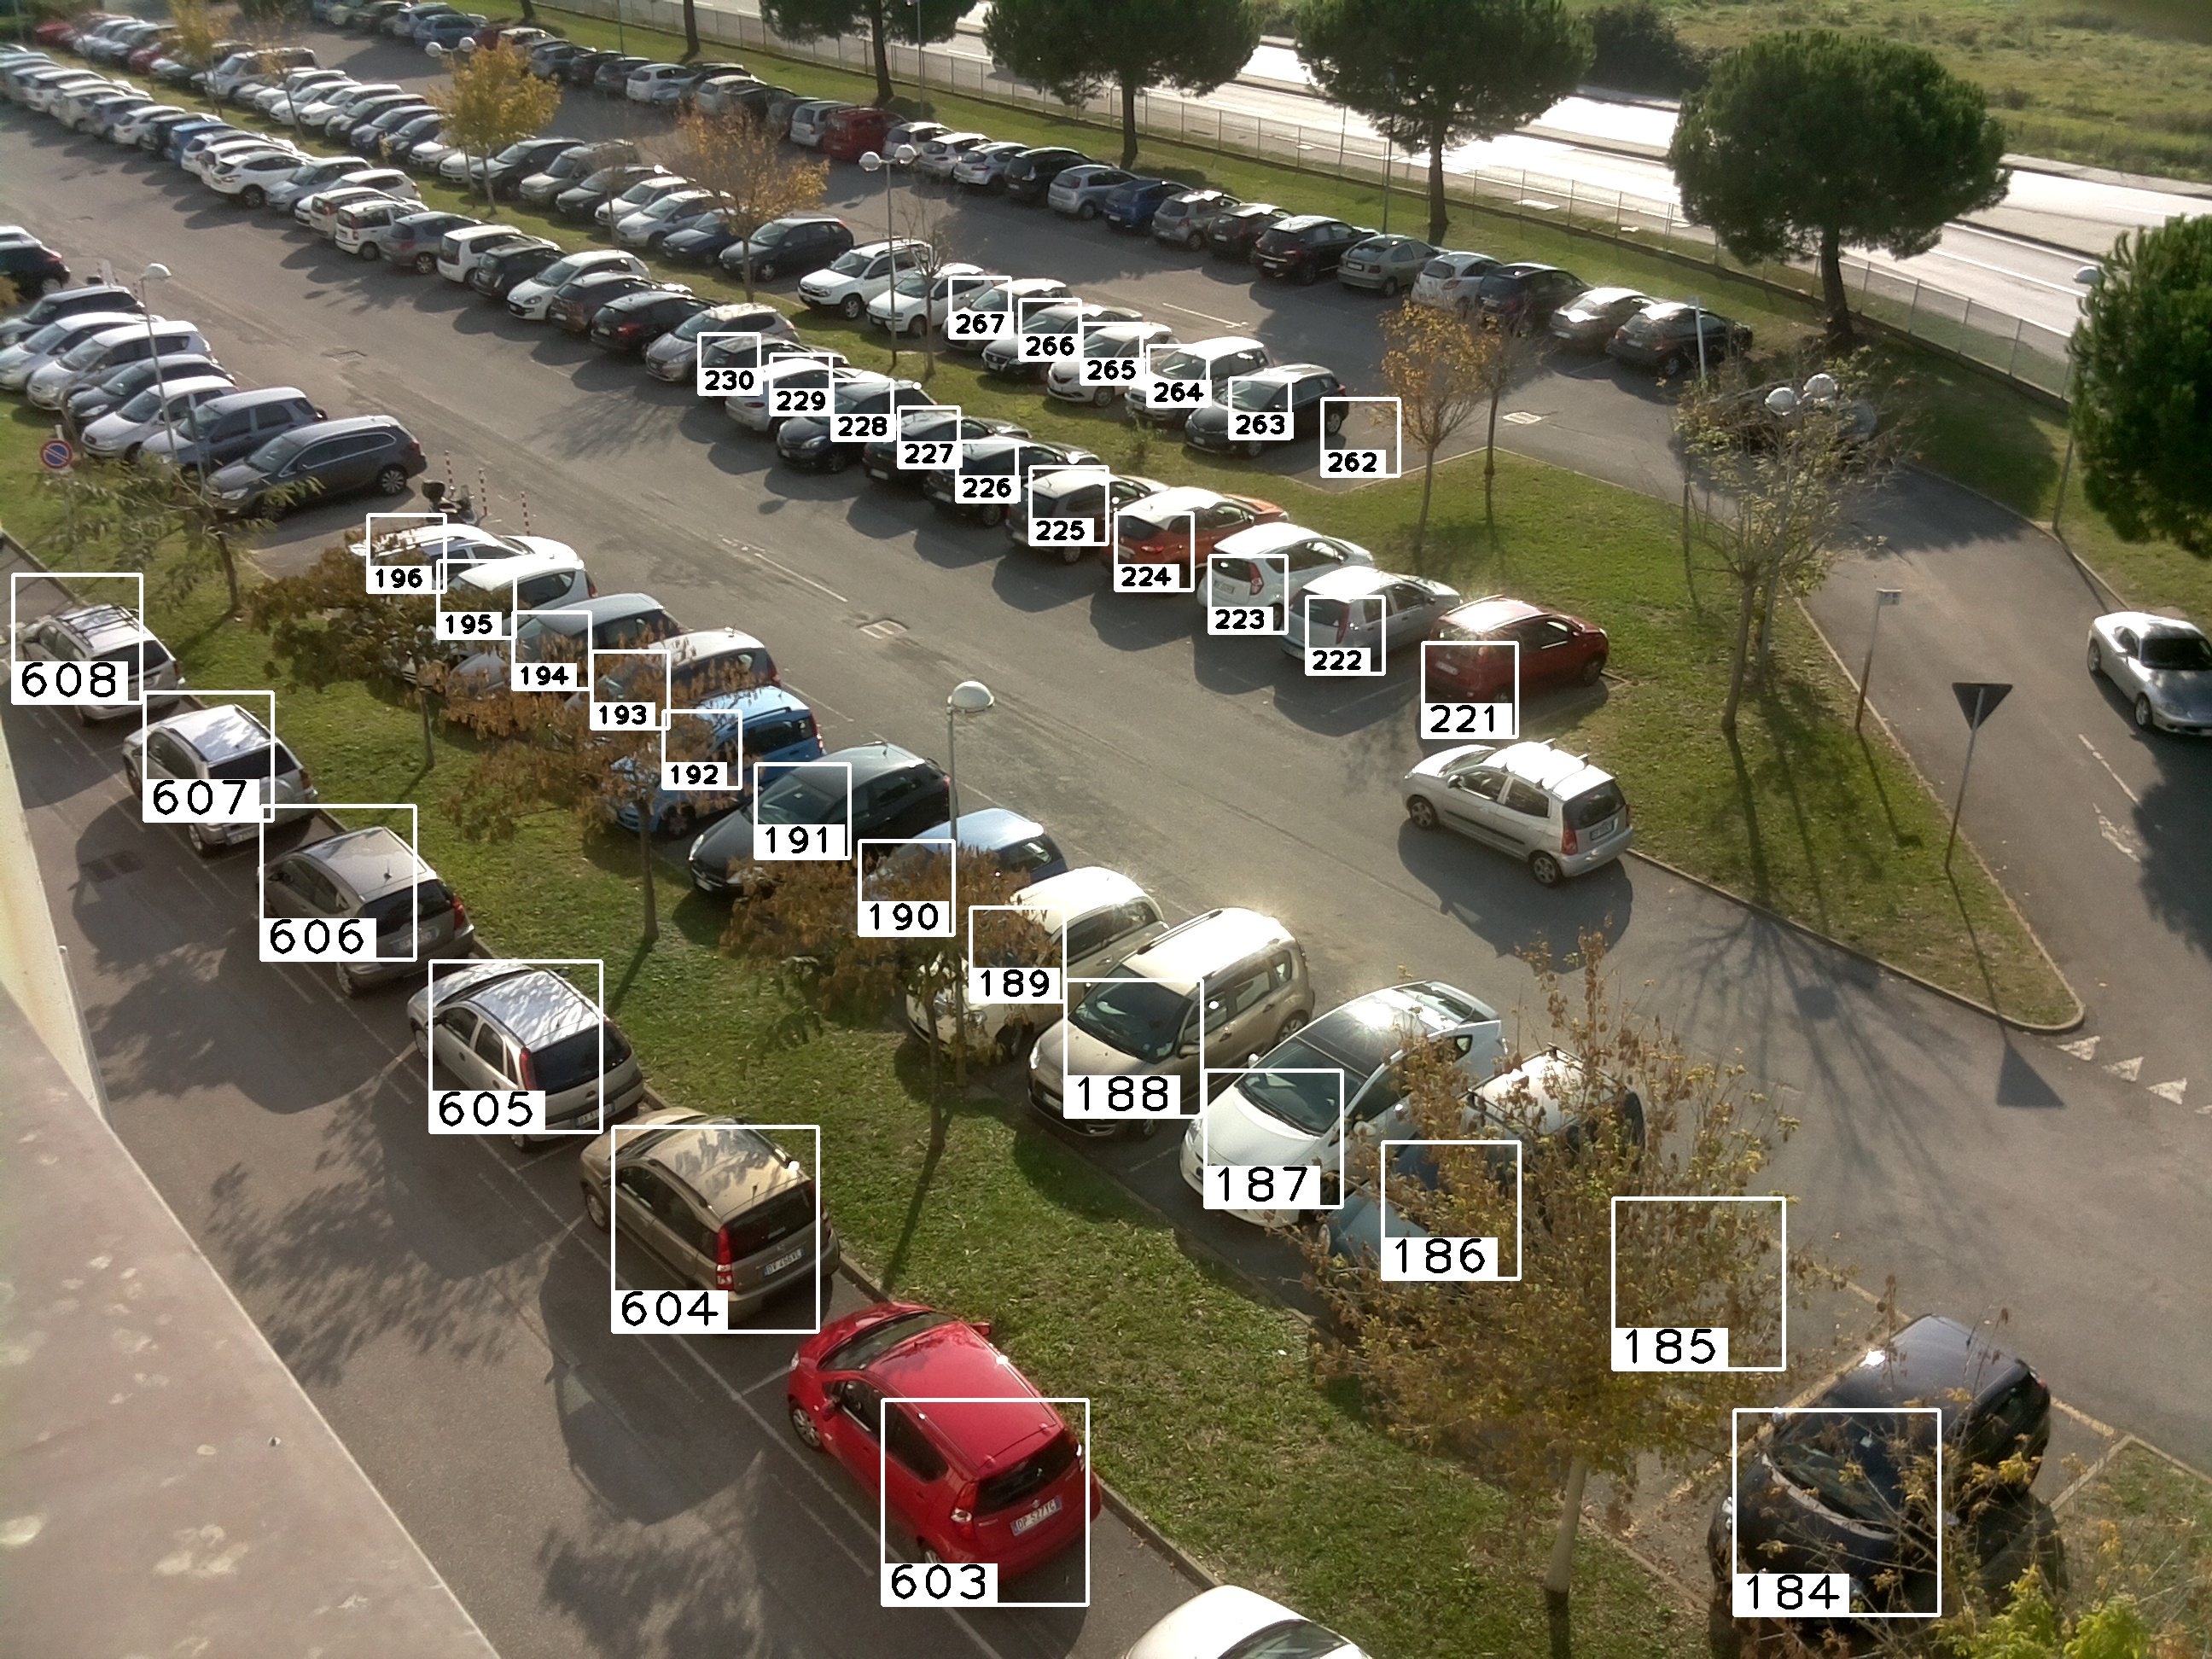
\includegraphics[width=\columnwidth]{overview-cam1}
	\caption{Overview of CNRPark-EXT CAM 1}
	\label{fig:mini:cam-1}
\end{subfigure} %
\begin{subfigure}[b]{0.49\columnwidth}
	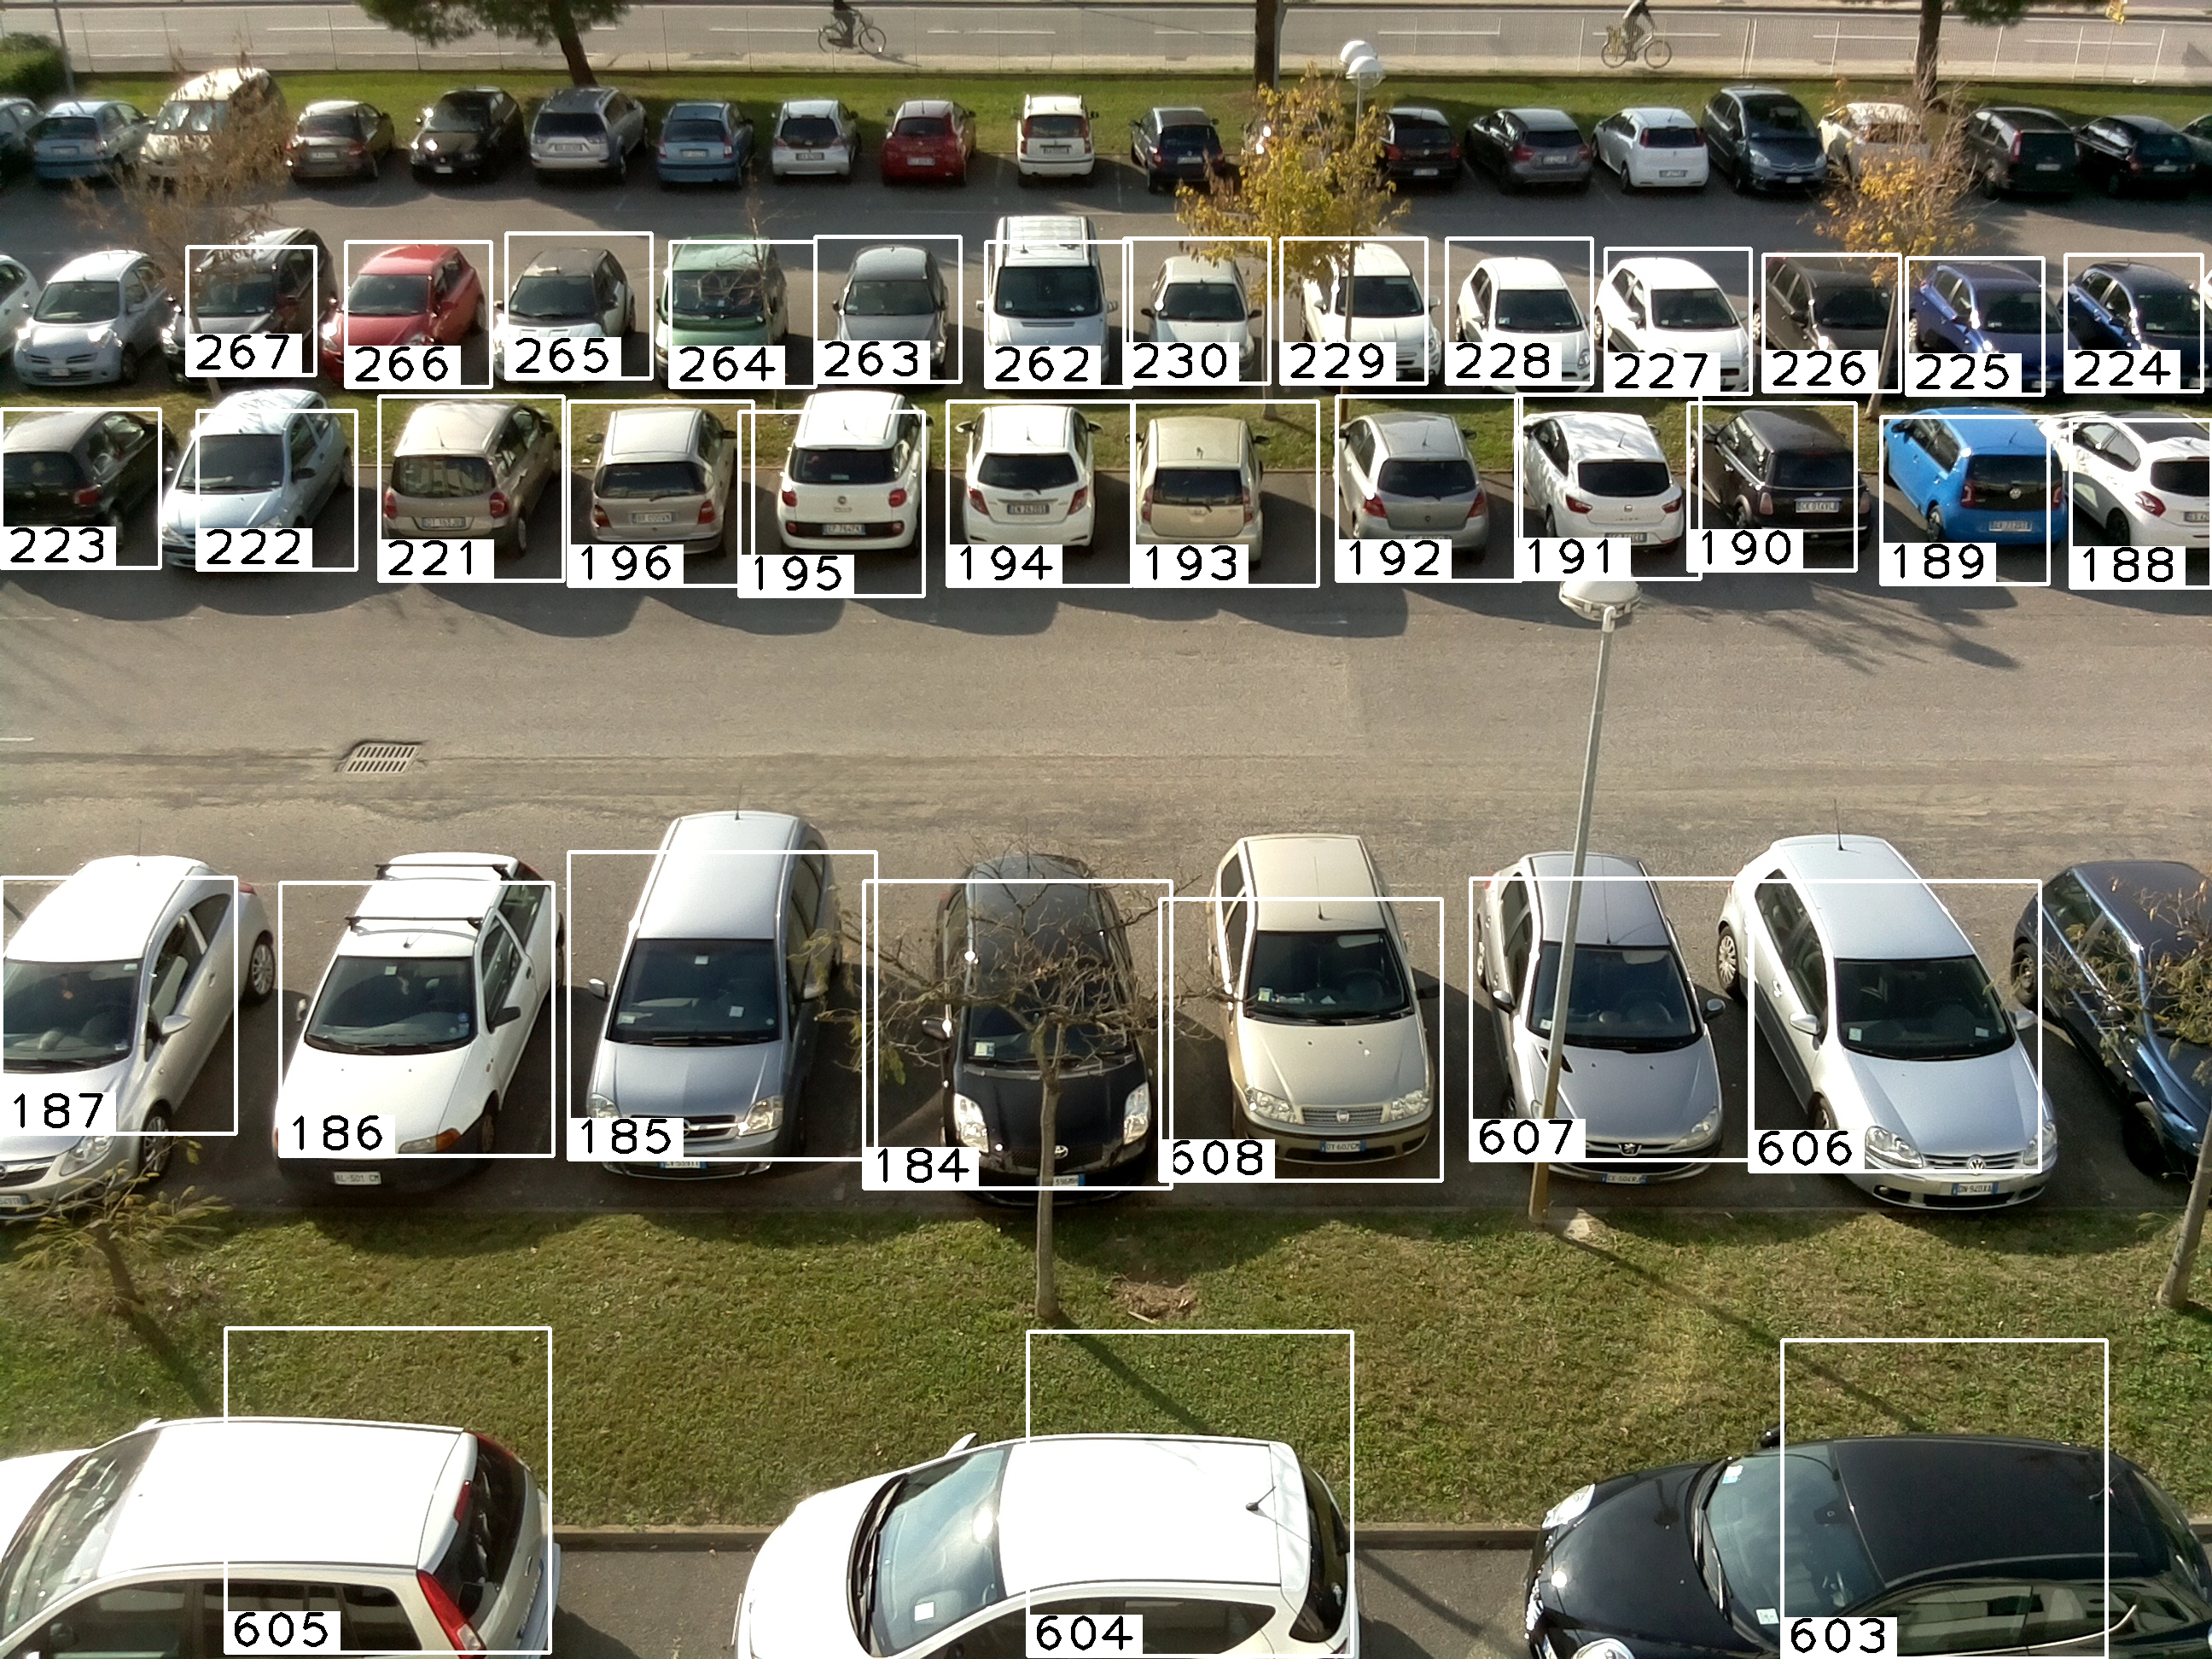
\includegraphics[width=\columnwidth]{overview-cam8}
	\caption{Overview of CNRPark-EXT CAM 8}
	\label{fig:mini:cam-8}
\end{subfigure}
\caption{Segmentation masks for parking slot images in the preliminary \emph{CNRPark} dataset (top) and in the extended \emph{CNRPark-EXT} dataset (bottom, only for camera 1 and 8)}
\label{fig:mini:cam-overview}
\end{figure}

\begin{figure}
\begin{subfigure}{0.25\columnwidth}%
\includegraphics[width=\columnwidth]{38busy}%
\end{subfigure}%
\begin{subfigure}{0.25\columnwidth}%
\includegraphics[width=\columnwidth]{34busy}%
\end{subfigure}%
\begin{subfigure}{0.25\columnwidth}%
\includegraphics[width=\columnwidth]{11busy}%
\end{subfigure}%
\begin{subfigure}{0.25\columnwidth}%
\includegraphics[width=\columnwidth]{13busy}%
\end{subfigure}

\begin{subfigure}{0.25\columnwidth}
\includegraphics[width=\columnwidth]{38empty}%
\end{subfigure}%
\begin{subfigure}{0.25\columnwidth}%
\includegraphics[width=\columnwidth]{34empty}%
\end{subfigure}%
\begin{subfigure}{0.25\columnwidth}%
\includegraphics[width=\columnwidth]{11empty}%
\end{subfigure}%
\begin{subfigure}{0.25\columnwidth}%
\includegraphics[width=\columnwidth]{13empty}%
\end{subfigure}
\caption{Example of segmented parking slots images under different light conditions and occlusion patterns.
The first and second rows show four slots respectively in `occupied` and `vacant` state}
\label{fig:mini:slots}
\end{figure}

\paragraph{CNRPark}
In order to measure the generalization power of the proposed approach to unseen scenarios, we personally built a new dataset --- named \emph{CNRPark} --- collecting images from the parking lot in the campus of the National Research Council (CNR) in Pisa.
The preliminary version of this dataset --- which we refer to as CNRPark --- contains roughly $12,000$ images of slots of a part of the parking lot which were collected from 2 Rasperry Pi cameras (denoted as camera $A$ and $B$) with different perspectives and angles of view in different days of July 2015 (see \ref{fig:mini:cam-a,fig:mini:cam-b}).
Images of individual parking slots are extracted using manually-placed squared masks from the full camera frame.
Slot masks are placed to minimize the part of adjacent slots contained in the image, often limiting the area usable for classification to just a part of the entire slot.
Moreover, in many slots, occlusions by adjacent cars and obstacles (e.g.\ trees, lampposts) are inevitable due to the skewed field of view of the cameras;
this also involves that slots images have different sizes depending on the distance of the slot from the capturing camera.
Thus, our dataset poses additional challenges to occupancy detection methods that can be commonly found in real scenarios.
We split the dataset in two non-overlapping sets named \emph{CNRParkOdd} and \emph{CNRParkEven} respectively containing slot images having odd or even slot id.
This permitted us to test the generalization of our approach by training on some slots and test on unseen slots.

\paragraph{CNRPark-EXT}
We subsequently extended the CNRPark dataset gathering more images of the complete parking lot --- comprised by 164 parking slots --- captured by 9 additional cameras from November 2015 to February 2016.
\ref{fig:mini:cam-1,fig:mini:cam-8} report the cameras with respectively the most and least skewed views.
Images were collected in multiple days spanning multiple seasons of the year, and the number of slots monitored by each camera roughly spans from 10 to 50.
To extract the images of individual slots, we followed the same strategy of CNRPark.
The extended version of the dataset --- dubbed \emph{CNRPark-EXT} -- is composed of 4,287 camera frames acquired in 23 different days, from which we obtained 144,965 manually labeled images of individual parking slots.
The added value of our dataset stands in the fact that it captures a variety of occlusion and shadow patterns, and light and weather conditions (see \ref{fig:mini:slots}) that cover more real-case scenarios with respect to existing datasets.
Slot images are grouped by camera ID, by time of capture, and by three weather conditions --- i.e.\ \emph{Sunny}, \emph{Overcast}, and \emph{Rainy}.
We also provide splits for training, validation, and test sets;
we ensured that images captured in a particular day do not span more than one set.

\ref{tab:mini:datasets} reports detailed information about the composition of \emph{CNRPark}, \emph{CNRPark-EXT}, and \emph{PKLot}~\cite{de2015pklot}.
The main difference between our datasets and the existing ones can be summarized as follows.
Slot images in \emph{CNRPark-EXT} often do not cover precisely or entirely the parking slot volume, whereas in \emph{PKLot} slots are registered and straightened, resulting in a more precise coverage of the parking slot.
Moreover, \emph{CNRPark-EXT} captures heavily occlusion patterns (some slots are almost entirely covered by trees and lampposts) and lower point of views, resulting in considerable occlusions due to adjacent vehicles.
Even if our dataset counts less images than \emph{PKLot} and has been collected from a single parking lot, we assessed through experiments that the real challenge comes from the variety of view-points and occlusions patterns of which our dataset is rich:
in fact, we let the \gls{cnn} to cope with these factors, resulting in a more robust classifiers in real case scenarios and in a reduced manual setup effort.

\begin{table}
\newcolumntype{R}{>{\raggedleft\arraybackslash}X}
% \def\arraystretch{1}
\begin{tabularx}{\linewidth}{lRRR}
\toprule
\textsc{Dataset}    & \textsc{vacant} & \textsc{occupied} & \textsc{total} \\
\midrule
%                       &               &               &                \\
%    CNRPark $A$       & 2549          & 3622          & 6171           \\
%    CNRPark $B$       & 1632          & 4781          & 6413           \\ \hline
%    CNRPark           & 4181          & 8403          & 12584          \\

     CNRPark           & 4,181          & 8,403          & 12,584          \\
     CNRPark-EXT       & 65,658         & 79,307         & 144,965         \\
     PKLot             & 337,780        & 358,119        & 695,899         \\ %\hline
%                       &               &               &                \\
%    CNRPark TRAIN     & 2201          & 3970          & 10000          \\
%    CNRPark VAL       & 1980          & 4433          & 2584           \\ \hline
%    CNRPark           & 4181          & 8403          & 12584          \\
\bottomrule
                       &               &               &                \\
\toprule
\textsc{Subset} & \textsc{vacant} & \textsc{occupied} & \textsc{total} \\ \midrule
    CNRParkOdd        & 2,201          & 3,970          & 6,171           \\
    CNRParkEven       & 1,980          & 4,433          & 6,413           \\ %hline
\midrule
     CNRPark-EXT TRAIN     & 46,877         & 47,616         & 94,493          \\
     CNRPark-EXT VAL       & 5,232          & 13,415         & 18,647          \\
     CNRPark-EXT TEST      & 13,549         & 18,276         & 31,825          \\ %\hline
%     CNRPark-EXT           & 65658         & 79307         & 144965         \\
\midrule
     CNRPark-EXT SUNNY     & 25,665         & 37,513         & 63,178          \\
     CNRPark-EXT OVCST     & 21,067         & 23,176         & 44,243          \\
     CNRPark-EXT RAINY     & 18,926         & 18,618         & 37,544          \\ %\hline
%     CNRPark-EXT           & 65658         & 79307         & 144965         \\
\midrule
     CNRPark-EXT \emph{C1}      & 6,407          & 9,308          & 15,715          \\
     CNRPark-EXT \emph{C2}       & 1,454          & 2,641          & 4,095           \\
     CNRPark-EXT \emph{C3}       & 4,101          & 5,370          & 9,471           \\
     CNRPark-EXT \emph{C4}       & 7,219          & 9,357          & 16,576          \\
     CNRPark-EXT \emph{C5}       & 9,582          & 11,256         & 20,838          \\
     CNRPark-EXT \emph{C6}       & 9,462          & 10,646         & 20,108          \\
     CNRPark-EXT \emph{C7}       & 10,595         & 10,519         & 21,114          \\
     CNRPark-EXT \emph{C8}       & 11,237         & 12,847         & 24,084          \\
     CNRPark-EXT \emph{C9}       & 5,601          & 7,363          & 12,964          \\ %\hline
%     CNRPark-EXT           & 65658         & 79307         & 144965         \\
\midrule
%					   &               &               &                \\
     PKLot2Days        & 27,314         & 41,744         & 69,058          \\
     PKLotNot2Days     & 310,466        & 316,375        & 626,841         \\ %\hline
%     PKLot             & 337780        & 358119        & 695899         \\
%                       &               &               &                \\
\midrule
     PKLot UFPR04 TRAIN& 25,894         & 23,266         & 49,160          \\
     PKLot UFPR04 TEST & 33,824         & 22,859         & 56,683          \\
     PKLot UFPR05 TRAIN& 45,759         & 48,196         & 93,955          \\
     PKLot UFPR05 TEST & 22,600         & 49,230         & 71,830          \\
     PKLot PUC TRAIN   & 114,424        & 106,334        & 220,758         \\
     PKLot PUC TEST    & 115,616        & 87,895         & 203,511         \\ %\hline
%     PKLot             & 337780        & 358119        & 695899         \\
%                       &               &               &                \\
\midrule
     PKLot TRAIN       & 27,314         & 41,744         & 105,843         \\
     PKLot VAL         & 54,909         & 47,453         & 165,785         \\
     PKLot TEST        & 275,894        & 248,583        & 424,269         \\ %\hline
%     PKLot             & 337780        & 358119        & 695899         \\
\bottomrule
  \end{tabularx}
\caption{Details of datasets used in the experiments, with the various proposed subsets.
Values refer to the number of slot images contained in every dataset or subset}
\label{tab:mini:datasets}
\end{table}

\section{Evaluation}
\label{sec:mini:evaluation}

In this section, we present the experimental evaluation and discuss the obtained results.
Our investigation focused on getting insight on three main aspects of the proposed solution that can be summarized by the following questions:
\begin{enumerate}
\item How does our reduced classifier compare against state-of-the-art approaches?
\item How much the generalization performance degrades when using our reduced model instead of the original AlexNet architecture?
\item How much the proposed solution for visual occupancy detection is robust to weather and viewpoint changes?
\end{enumerate}

To answer these question, we extensively evaluated our approach using the two datasets described in \ref{sec:mini:datasets}, i.e.\ PKLot and CNRPark-EXT.
We performed experiments by splitting the datasets into several subsets that we will described in the following subsections.
Details about data splits are summarized in \ref{tab:mini:datasets}.
The usage of multiple methods on multiple datasets also permits us to compare the quality of our newly collected dataset for learning to detect occupancy detection robustly in real scenarios.

% -----

\subsection{Comparison with the State of the Art}
\label{sub:mini:sota}

We compared \emph{mAlexNet} against the state-of-the-art visual occupancy detection system proposed by \citet{de2015pklot}, which is based on \glspl{svm} classifiers with RBF kernels defined over hand-crafted textural features.
Specifically, histograms of \gls{lbp}, \gls{lpq} features and their variations \cite{ojala2002multiresolution, ojansivu2008blur, rahtu2012local} have been tested as input features of the \gls{svm}.
\Glspl{svm} are calibrated to output the probability of a slot to be occupied.
The authors also shown that the performance of the classification can be improved by using ensembles of \gls{svm} classifiers each defined on a particular textural feature:
probability values are fused using simple aggregation functions, such as \emph{Max} and \emph{Mean}, to obtain the final decision for an image slot.

We follow the experimental protocol described in \cite{de2015pklot}.
We split images from each camera of the PKLot dataset (UFPR04, UFPR05, and PUC) into a training and test set with roughly a 50\%--50\% proportion;
for a fair evaluation, we ensure that images collected in a particular day do not appear in both training and test set.
We then train both mAlexNet and the \glspl{svm} on each of the three training set, and tested on all the available test sets.
%
%Similarly, we also repeated the same protocol with our preliminary CNRPark dataset.
%We split CNRPark into two subsets --- CNRParkEven and CNRParkOdd --- respectively containing images of slots having even and odd IDs.
%We train both \glspl{svm} and mAlexNet on one subset and test on the other, and vice-versa.

For each experiment, we evaluated the prediction obtained for the test set by measuring the percentage error (\textbf{Err. \%}), defined as $100 \cdot (1 - \text{Accuracy})$, and the \gls{roc} \textbf{\gls{auc}}.
The former gives us an overall evaluation of the systems assuming a slot is occupied if the probability is above $0.5$, while the latter summarize the behaviour of the systems independently from the probability threshold chosen.


\paragraph{Training and implementation details for mAlexNet}
Input images are squashed to a resolution of $256\times256$ before being fed to the network.
During the training phase, we perform data augmentation by taking a $224\times224$ random crop of the resized image and flipping it horizontally with $\sfrac{1}{2}$ probability.
In the test phase, images are resized to $224\times224$ resolution and no flipping is performed.
All the mAlexNet models are trained with \gls{sgd} with momentum for 18 epochs, with a learning rate of $0.01$ halved every 6 epochs, a batch size of $64$, a momentum of $0.9$, and a weight decay of $5e^{-4}$;
due to the low model complexity, no dropout regularization is used.
To avoid overfit on the test set, we validate our models at each training epoch by evaluating it on a validation set.
As validation sets, we used the training splits of the PKLot cameras --- e.g.\ when testing on PUC test subset, we use PUC training subset as validation set.
We choose as final model for a particular dataset the one which performs best on the validation test.

\paragraph{Training and implementation details for \glspl{svm}}
To train the \glspl{svm}, we employ the procedure and the hyper-parameters as described by \citet{de2015pklot} here summarized.
We extract LBP-type features with a radius of 1 and 8 neighbors.
LPQ features are extracted using window size of 3x3.
The $C$ and $\gamma$ parameters of \glspl{svm} are chosen with grid search and a 5-fold cross-validation on the training set.
We choose the parameters $(C,\gamma)$ obtaining the best 5-fold accuracy, i.e.\ the best accuracy obtained classifying each fold of the dataset with the model trained on the other folds.
The final SVM is then trained on the entire training set using the chosen parameters, and evaluated on the test set.
We followed the same strategy used in \cite{de2015pklot} to obtain a probabilistic score from the output of the \gls{svm}, which evaluates the posterior probability fitting a sigmoid function with two parameters \cite{platt1999probabilistic}.

\begin{table}
    \newcolumntype{C}{>{\centering\arraybackslash}X}
    \begin{tabularx}{\linewidth}{lcX}
        \toprule
        \textsc{Method} & \textsc{Input Dim.}     & \textsc{Input Description} \\
        \midrule
        mAlexNet         & $224\times 224\times 3$ & a 224x224 RGB image \\
        SVM + LBP        & $256$                     & histograms of classical \acrfull{lbp} \cite{ojala2002multiresolution} \\
        SVM + LBPu       & $59$                      & histograms of uniform LBP \cite{ojala2002multiresolution} \\
        SVM + LBPri      & $36$                      & histograms of rotational invariant LBP \cite{ojala2002multiresolution}  \\
        SVM + LBPuri     & $10$                      & histograms of uniform and rotational invariant LBP \cite{ojala2002multiresolution} \\
        SVM + LPQu       & $256$                     & histograms of \acrfull{lpq} (uniform initialization) \cite{ojansivu2008blur} \\
        SVM + LPQg       & $256$                     & histograms of LPQ (gaussian initialization) \cite{rahtu2012local} \\
        SVM + LPQgd      & $256$                     & histograms of LPQ (gaussian derivative initialization) \cite{rahtu2012local} \\
        \bottomrule
     \end{tabularx}
     \caption{Summary of state-of-the-art methods compared against our approach for parking slot occupancy detection}
     \label{tab:mini:methods}
\end{table}

\begin{table}
	\newcolumntype{R}{>{\raggedleft\arraybackslash}X}

	\begin{tabularx}{\linewidth}{lRRRRRR}
	\toprule
	\textsc{Method}               & \multicolumn{2}{c}{\textsc{UFPR04}} & \multicolumn{2}{c}{\textsc{UFPR05}}  & \multicolumn{2}{c}{\textsc{PUC}}  \\
								    \cmidrule(lr){2-3}  \cmidrule(lr){4-5}   \cmidrule(lr){6-7}
	\textbf{Train on UFPR04}      & \textbf{Err. \%} & \textbf{AUC} & \textbf{Err. \%} & \textbf{AUC} & \textbf{Err. \%} & \textbf{AUC} \\
	\midrule
	mAlexNet                      & 0.46 & 0.99      & 6.71  & 0.99    & 1.73  & 0.99 \\
	LPQu / LPQg / LPQg*           & 0.45 & 0.99      & 15.08 & 0.94    & 15.75 & 0.94 \\
	Mean / Max / Max Ensemble*    & 0.36 & 0.99      & 11.67 & 0.95    & 11.60 & 0.95 \\
	\midrule
	\textbf{Train on UFPR05}      & \textbf{Err. \%} & \textbf{AUC} & \textbf{Err. \%} & \textbf{AUC} & \textbf{Err. \%} & \textbf{AUC} \\
	\midrule
	mAlexNet                      &  6.31 & 0.98     & 0.51 & 0.99     & 7.28  & 0.98 \\
	LPQgd / LPQu / LPQu*          & 14.24 & 0.93     & 1.10 & 0.99     & 12.26 & 0.94 \\
	Mean  Ensemble*               & 14.47 & 0.95     & 0.70 & 0.99     & 10.17 & 0.97 \\
	\midrule
	\textbf{Train on PUC}         & \textbf{Err. \%} & \textbf{AUC} & \textbf{Err. \%} & \textbf{AUC} & \textbf{Err. \%} & \textbf{AUC} \\
	\midrule
	mAlexNet                      &  1.97 & 0.99     & 4.00  & 0.99    & 0.10 & 0.99 \\
	LPQg / LBPri / LPQu*          & 12.85 & 0.94     & 17.22 & 0.91    & 0.42 & 0.99 \\
	Mean  Ensemble*               & 11.12 & 0.95     & 15.80 & 0.91    & 0.39 & 0.99 \\
	\bottomrule
	\end{tabularx}

%	\begin{tabularx}{\linewidth}{XRRRR}
%	\toprule
%	                              & \multicolumn{2}{c}{\textsc{CNRParkEven}} & \multicolumn{2}{c}{\textsc{CNRParkOdd}} \\
%	\textsc{Method}               & \multicolumn{2}{c}{\textbf{\small Train on CNRParkOdd}} & \multicolumn{2}{c}{\textbf{\small Train on CNRParkEven}} \\
%									\cmidrule(lr){2-3}                         \cmidrule(lr){4-5}
%								  & \textbf{Err. \%} & \textbf{AUC} & \textbf{Err. \%} & \textbf{AUC} \\
%	\midrule
%	mAlexNet                      & 9.87 & 0.94 & 9.29 & 0.92  \\
%	LPQgd / LBP*                  & 12.35 & 0.95 & 12.79 & 0.92 \\
%	\bottomrule
%	\end{tabularx}

	\caption{Comparison of \emph{mAlexNet} against state-of-the-art approaches presented by \citet{de2015pklot}}
	\label{tab:mini:net-vs-svms}
\end{table}

A summary of the compared methods is reported in \ref{tab:mini:methods}, and results are reported in \ref{tab:mini:net-vs-svms}.
For simplicity, we report for each experiment only the variant of LBP or LPQ that yielded the best performance on each subset, and for ensembles, we report instead the best aggregation function.
We can notice that \emph{mAlexNet} generally perform better then other compared methods in terms of both percentage error and AUC.
All the methods perform well when training and test images comes from the same camera;
in fact, most of them reach a classification error less than 1\%.
However, our \gls{cnn}-based solution exhibits a stronger generalization power, reaching errors 3--10\% lower when training and test images comes from different cameras.
% In fact, \emph{mAlexNet} reaches accuracy values of 98.27\% in the UFPR04/PUC training/test set configuration.
% This is roughly $10\%$ more accurate than the best compared method, that is \emph{Max Ensemble}, which reaches 88.40 \%.

To stress test the generalization capabilities, we also performed experiments when training and test sets comes from completely different dataset, which is a common assumption in the setup and deployment of real systems.
We used both PKLot and CNRPark dataset respectively as training and test set, and vice-versa.
To reduce training times of \glspl{svm}, we used a smaller subset of PKLot as training set --- named PKLot2Days --- obtained by selecting images captured in the first two days in chronological order for each camera (UFPR04, UFPR05, and PUC) and for each weather condition (SUNNY, OVERCAST, RAINY) available.
The test phase is still performed on the whole PKLot dataset.

\begin{table}
  \newcolumntype{R}{>{\raggedleft\arraybackslash}X}
  \begin{tabularx}{\linewidth}{lRRRR}
  \toprule
                                & \multicolumn{2}{c}{\textsc{CNRPark}} & \multicolumn{2}{c}{\textsc{PKLot}} \\
  \textsc{Method}               & \multicolumn{2}{c}{\textbf{\small Train on PKLot2Days}} & \multicolumn{2}{c}{\textbf{\small Train on CNRPark}} \\
                                  \cmidrule(lr){2-3}                              \cmidrule(lr){4-5}
                                & \textbf{Err. \%} & \textbf{AUC}               & \textbf{Err. \%} & \textbf{AUC} \\
  \midrule
  mAlexNet                      & 17.12            & 0.899                      &  9.62            & 0.989 \\
  LPQu                          & 35.36            & 0.447                      & 60.18            & 0.743 \\
  LPQgd                         & 38.26            & 0.465                      & 59.01            & 0.601 \\
  LPQg                          & 36.16            & 0.450                      & 56.19            & 0.599 \\
  LBPuri                        & 34.69            & 0.580                      & 50.26            & 0.496 \\
  LBPu                          & 35.73            & 0.506                      & 53.33            & 0.450 \\
  LBPri                         & 35.80            & 0.556                      & 51.28            & 0.405 \\
  LBP                           & 36.87            & 0.491                      & 47.12            & 0.391 \\
  \bottomrule
  \end{tabularx}

  \caption{Cross-dataset experiments performed to stress test the generalization performance of compared methods.}
  \label{tab:mini:x-dataset}
\end{table}

Results in \ref{tab:mini:x-dataset} clearly show how features learned by the \gls{cnn} are more transferable to different domains with respect to the manually engineered textural features.
Moreover, as expected, classifying the CNRPark dataset while training on PKLot is more challenging than its counterpart.
Despite being smaller, the higher variability and the additional occlusion patterns captured by our dataset comprises a richer training set for learning-based methods.
In fact, the whole PKLot can be annotated with roughly 10\% error while training on CNRPark which contains $60\times$ less images.
Again, \emph{mAlexNet} still outperforms the other compared classifiers in this configuration.
As stated by \citet{de2015pklot}, we do not observed an absolute best textural feature among the tested one.
% However, we noticed that in most of the cases, LPQu and LPQg (Local Phase Quantization with respectively uniform and Gaussian initialization), give better performance.
% We noticed in their results that taking the mean of the confidence coming from different classifiers (to which we refer with \emph{Mean Ensemble}) usually improves the performance.

% We also report the experiments performed in a preliminary work \cite{amato2016car} in which we
% compared \emph{mAlexNet} to the techniques proposed in \cite{de2015pklot} using \emph{CNRPark} dataset.
% For each experiment, we report only the variant of LBP or LPQ that yielded the best performance.

\subsection{Evaluation of the generalization between datasets}
\label{sub:mini:generalization}

In this section, we describe the experiments and results we performed to compare the generalization performance of our reduced \gls{cnn} architecture against the original AlexNet architecture.

To measure the generalization performance, we train both models on a dataset, and we evaluate the trained models on a different one, in which images are coming from a different parking lot and have different camera height and pose.
We perform multiple experiments using different sets of images to also measure the generalization power obtained by datasets with different degree of variability.
As training sets, we separately employed \emph{CNRPark}, \emph{CNRPark} plus cameras \emph{C1} and \emph{C8} of \emph{CNRPark-EXT}, \emph{CNRPark-EXT}, and \emph{PKLot}.
Validation is performed on the corresponding validation sets, while evaluation metrics --- i.e.\ percentage error and \gls{auc} --- are reported for CNRPark-EXT and PKLot test sets.
The set composed by \emph{CNRPark} plus cameras \emph{C1} and \emph{C8} of \emph{CNRPark-EXT} is chosen to built a balanced set of different viewpoints.
While \emph{CNRPark-EXT} is comprised by 9 different cameras, most of them share the same frontal view-point of the parking lot.
Thus, we selected \emph{C1} and \emph{C8} --- which have the most dissimilar views of the parking lot --- and we combined them with CNRPark, which is composed by other two different view-points (see \ref{fig:mini:cam-overview}).

All the models are trained for 6 epochs, with a learning rate of $8e^{-4}$, which is multiplied by $0.75$ every 2 epochs.
Other hyper-parameters are the following: batch size $64$, momentum $0.9$, and weight decay $5e^{-4}$.
The final models are chosen as the ones obtaining the best performance on the validation sets.
Details about the subsets used in these experiments are reported in \ref{tab:mini:datasets}.

% In experiments 1.1 and 1.2, we measured how much predictive power both models can obtain from the \emph{PKLot} dataset.
% We splitted both the \emph{PKLot} and \emph{CNRPark-EXT} datasets in TRAIN/VAL/TEST subsets picking images from different days from all the weather conditions.
% We trained both networks on the \emph{PKLot TRAIN}, using use \emph{PKLot VAL} and \emph{CNRPark-EXT VAL} as validation sets.
% We then computed the accuracy of those two trained models on \emph{PKLot TEST} and \emph{CNRPark-EXT TEST}.

% We then measured the informativeness of our preliminary dataset \emph{CNRPark}, following the same methodology for experiments 2.1 and 2.2.
% We trained both models using \emph{CNRPark} as training set, \emph{CNRPark-EXT VAL} and \emph{PKLot VAL} as validation sets, and we tested on \emph{CNRPark-EXT TEST} and \emph{PKLot TEST}.

% In experiments 3.1 and 3.2, we replicated experiments 2.1 and 2.2, using the extended dataset \emph{CNRPark-EXT}.
% The training set is composed by the whole \emph{CNRPark} plus \emph{CNRPark-EXT TRAIN}, named \emph{CNRPark+EXT TRAIN} for brevity.
% % \emph{CNRPark-EXT VAL} was used as validation set instead of \emph{CNRPark VAL}.

% In experiments 4.1 and 4.2, we replicated experiments 3.1 and 3.2, using a more balanced training set in terms of viewpoints.
% In \emph{CNRPark+EXT TRAIN}, the majority of the images are captured  from a frontal viewpoint.
% We selected only two cameras from \emph{CNRPark-EXT TRAIN}, camera 1 and camera 8, that have the most different viewpoints of the parking lot.
% Thus we obtained a balanced number of images from different viewpoints.
% We added those images to \emph{CNRPark}, forming a new balanced training set, named \emph{CNRPark+EXT TRAIN C1-C8}.

\begin{table}
  \newcolumntype{R}{>{\raggedleft\arraybackslash}X}

  \begin{tabularx}{\linewidth}{lRRRR}
  \toprule
  \textsc{Method}               & \multicolumn{2}{c}{\textsc{CNRPark-EXT TEST}} & \multicolumn{2}{c}{\textsc{PKLot TEST}} \\
                                  \cmidrule(lr){2-3}                              \cmidrule(lr){4-5}
  \textbf{Train on CNRPark}     & \textbf{Err. \%} & \textbf{AUC}               & \textbf{Err. \%} & \textbf{AUC} \\
  \midrule
  mAlexNet                      & 6.48             & 0.9838                     & 4.72             & 0.9916 \\
  AlexNet                       & 6.37             & 0.9877                     & 4.40             & 0.9910 \\
  \midrule

  \textbf{Train on CNRPark+EXT TRAIN C1,C8} & \textbf{Err. \%} & \textbf{AUC}   & \textbf{Err. \%} & \textbf{AUC} \\
  \midrule
  mAlexNet                      & 4.12             & 0.9937                     & 9.52             & 0.9738 \\
  AlexNet                       & 3.15             & 0.9957                     & 3.49             & 0.9937 \\
  \midrule

  \textbf{Train on CNRPark+EXT TRAIN} & \textbf{Err. \%} & \textbf{AUC}         & \textbf{Err. \%} & \textbf{AUC} \\
  \midrule
  mAlexNet                      & 2.29             & 0.9967                     & 15.47            & 0.9699 \\
  AlexNet                       & 2.00             & 0.9974                     &  6.30            & 0.9923 \\
  \midrule

  \textbf{Train on PKLot TRAIN} & \textbf{Err. \%} & \textbf{AUC}    & \textbf{Err. \%} & \textbf{AUC} \\
  \midrule
  mAlexNet                      & 16.17            & 0.9139                     & 1.93             & 0.9967 \\
  AlexNet                       &  9.48            & 0.9684                     & 1.19             & 0.9984 \\
  \bottomrule
  \end{tabularx}

  \caption{Experiments performed to test the generalization performance of \emph{mAlexNet} and \emph{AlexNet}. Accuracies on test sets are reported, for each combination of model, training set, and test set.}
  \label{tab:mini:malex-vs-alex}
\end{table}

Results are reported in \ref{tab:mini:malex-vs-alex}.
We can notice that our reduced architecture does not suffer from a performance degradation with respect to the original \emph{AlexNet} when data comes from the same domain;
in fact, the percentage errors of both models differ at most of $1\%$ in all experiments where training and test subsets are taken from the same dataset.
When training and test is performed on different datasets, \emph{AlexNet} reaches higher accuracy values.
It is clear that the reduced architecture limits the degree of generalization the model can reach;
when using a viewpoint-balanced training set (i.e.\ \emph{CNRPark} and \emph{Train on CNRPark+EXT TRAIN C1,C8}), \emph{AlexNet} is able to reach a percentage error on \emph{PKLot} of $3.49\%$, while our method perform worse still obtaining less than 10\% error.

In the best case, there is practically no difference between the two methods, while in the worst case, we measured a difference of $\sim 9\%$ with respect to \emph{mAlexNet}.
Obviously, a bigger model offers a greater generalization performance at the cost of more resources needed:
the computation time for \emph{mAlexNet} --- measured on the Raspberry Pi model B --- allows to perform a classification in roughly $300ms$, while \emph{AlexNet} takes roughly $20s$.

\subsection{Evaluation of the generalization between cameras and weather}

%Errors in the occupancy detection of parking spaces are due to many reasons.
%For instance, the lighting condition changes during different periods of the year;
%moreover, occlusions and reflection patterns might introduce a fixed source of error.
%The weather condition might produce significant illumination changes as well.
%During a rainy weather, puddles and wet floor create textural patterns that may lead to a misclassification.
%Sunbeams can create reflections on the car's windscreen or on water, covering the majority of the images with saturated patterns.
%As we discussed in previous experiments, errors might also be due to low generalization properties of the classifier.
%When a classifier does not generalize well, it works well just in the conditions where it was trained.
%For instance, a bad classifier trained on a certain point of view of the parking lot, does not work well when tested with images coming from a camera seeing the parking lot from a different point of view.

The source of errors in classifiers for visual occupancy detection is manyfold.
The majority of errors comes from illumination changes due to variable weather and seasonal light changes;
examples of such conditions are cloud shadows, puddles and wet ground, sun reflections, etc.
Moreover, significant view-point changes between training data and real data is another suitable cause of performance degradation.

We measure the robustness of our approach to these scenarios performing \emph{inter-camera} and \emph{inter-weather} experiments.
With the former, we indicate experiments where we train on a particular viewpoint and test on other unseen viewpoints, while with the latter, we indicate experiments where we train using images collected during a particular weather condition --- sunny, overcast, or rainy ---, and we test on the others.

For both experiments, we employed our extended \emph{CNRPark-EXT} dataset.
For inter-camera experiments, we trained \emph{mAlexNet} using images of one camera among the 9 available, and measured the accuracy obtained on images coming from the other cameras.
We repeat this experiment using both the cameras with most and less skewed viewpoints (respectively \emph{C1} and \emph{C8}) to analyze the classifier robustness to challenging viewpoint changes.
For inter-weather experiments, we performed three experiments training respectively on \emph{CNRPark-EXT SUNNY}, \emph{OVERCAST}, and \emph{RAINY} subsets and evaluating the obtained classifiers on the other weather conditions.
For both kind of experiments, we report also the performance evaluated on the PKLot dataset for completeness.
The training procedure and hyperparameters strictly follow the one described in \ref{sub:mini:generalization}.

\begin{table}
\newcolumntype{R}{>{\raggedleft\arraybackslash}X}
\begin{tabularx}{\linewidth}{Xrrrrrrrrrr}
\toprule
\textsc{Train Set} &   \textsc{C1} &   \textsc{C2} &   \textsc{C3} &   \textsc{C4} &   \textsc{C5} &   \textsc{C6} &   \textsc{C7} &   \textsc{C8} &   \textsc{C9} & \textsc{PKLot} \\
                   \cmidrule(lr){2-2} \cmidrule(lr){3-3} \cmidrule(lr){4-4} \cmidrule(lr){5-5} \cmidrule(lr){6-6} \cmidrule(lr){7-7} \cmidrule(lr){8-8} \cmidrule(lr){9-9} \cmidrule(lr){10-10} \cmidrule(lr){11-11}
CNRPark-EXT C1 &    - & 5.15 & 6.89 & 4.00 & 4.09 & 4.39 & 8.57 & 5.39 & 9.04 & 26.92 \\
CNRPark-EXT C8 & 7.61 & 5.49 & 6.34 & 2.47 & 2.07 & 2.32 & 6.47 &    - & 5.35 &  4.51 \\
\bottomrule
\end{tabularx}
\caption{Results of inter-camera experiments in terms of accuracy obtained when training \emph{mAlexNet} on camera 1 and on camera 8}
\label{tab:mini:inter-camera}
% ALTERNATIVE FIG:
% \begin{figure}
% \includegraphics[width=\linewidth]{inter-camera}
% \caption{Results of inter-camera experiments in terms of accuracy obtained when training \emph{mAlexNet} on camera 1 (in blue), and on camera 8 (in red).}
% \label{fig:mini:inter-camera}
% \end{figure}
\end{table}

\begin{table}
\newcolumntype{R}{>{\raggedleft\arraybackslash}X}
\begin{tabularx}{\linewidth}{lRRRR}
\toprule
\textsc{Train Set} & \textsc{Sunny} & \textsc{Overcast} & \textsc{Rainy} & \textsc{PKLot} \\
                     \cmidrule(lr){2-2} \cmidrule(lr){3-3} \cmidrule(lr){4-4} \cmidrule(lr){5-5}
CNRPark-EXT SUNNY    &    - & 2.20  & 4.21 & 17.01 \\
CNRPark-EXT OVERCAST & 8.37 &    -  & 5.32 & 20.51 \\
CNRPark-EXT RAINY    & 6.47 & 1.73  &    - &  9.42 \\
\bottomrule
\end{tabularx}
\caption{Results of inter-weather experiments in terms of accuracy obtained when training on a sunny, overcast, or rainy weather}
\label{tab:mini:inter-weather}
% ALTERNATIVE FIG:
% \begin{figure}[t]
% \includegraphics[width=\columnwidth]{inter-weather}
% \caption{Results of inter-weather experiments in terms of accuracy obtained when training on a sunny (in blue), overcast (in red), or rainy (in yellow) weather.}
% \label{fig:inter-weather}
% \end{figure}
\end{table}

\ref{tab:mini:inter-camera,tab:mini:inter-weather} respectively report the percentage classification error values obtained in \emph{inter-camera} and \emph{inter-weather} experiments.
% The histograms compare the accuracy of a classifier trained on a specific scenario (a specific camera or a specific whether condition) when tested on all other possible scenarios.

In \emph{inter-camera} experiments, the model trained on \emph{C8} --- which has a clean anc central view of the parking lot --- exhibits the best performance on most of the other cameras since their viewpoint do no differ significantly;
in fact, the worst performance among all cameras is obtained on \emph{C1} --- which mainly captures partially occluded images and has the most skewed viewpoint that differs the most from \emph{C8}.
For the same reason, the model trained on \emph{C1} has a worse performance, but still is able to reach less than $10\%$ error on cameras coming from the same dataset.
The PKLot dataset is mainly composed by images with no occlusions and with a central and vertical view of the parking lots, and thus it is better classified by the model trained on \emph{C8}.

In \emph{inter-weather} experiments, we observed a strong generalization pattern.
Moreover, the performance degradation is directly related to the difference between training and testing weather conditions.
For example, when training on ``sunny'' images, we achieve better performance on ``overcast'' images than ``rainy'' ones.
Similarly, when training on ``rainy'' images, the model is more accurate on ``overcast' images than ``sunny'' ones.
Results on the \emph{PKLot} dataset show that light conditions play an important role on the classification performance;
in fact, we notice that these are similar between images in the \emph{PKLot} dataset and ``rainy'' images, which justifies the lower percentage error in the results.

\section{Deployment on CNR Pisa Parking Lot}
\label{sec:mini:deployment}

\begin{figure}
	\centering
    \begin{subfigure}{0.48\columnwidth}
		\includegraphics[width=\columnwidth]{camera_inside}
        \caption{Inside of a camera box}
	\end{subfigure} %
    \begin{subfigure}{0.48\columnwidth}
		\includegraphics[width=\columnwidth]{camera_box}
        \caption{The complete camera box}
	\end{subfigure}

	\caption{Each Raspberry Pi is mounted inside a outdoor camera box (Figure $A$ on the left) and it is mounted on top of the roof of the building, attached to a steel pole (Figure $B$ on the right)}
	\label{fig:mini:camera-box}
\end{figure}

\begin{figure}
	\centering
		\includegraphics[width=\columnwidth,trim={0 0 0 3.5ex},clip]{detection-example}
        \caption{Example of classification of a portion of the parking lot}
	\label{fig:mini:detection-example}
\end{figure}

In this section, we describe the details of the deployment of a prototype of our proposed solution for parking lot visual occupancy detection in the campus of the National Research Council (CNR) in Pisa.

We deployed 9 smart cameras on the roof of the building in front of a section of the campus parking lot.
Each smart camera is built from a Rasbperry Pi 2 model B equipped with standard Raspberry Pi camera module and mounted on an outdoor camera box (see \ref{fig:mini:camera-box}).
The total cost for a single camera is roughly 80\euro.
Hardware and software details are briefly reported for completeness.
The smart cameras are equipped with an ARM Cortex-A7 CPU, 1GB RAM DDR2, and a 32GB micro SD card for storage.
The camera module is a 5MP fixed-focus camera that supports 1080p30, 720p60 and VGA90 video modes, as well as still captures.
The view angles of the camera are 53.50$^{\circ}$ horizontally and 41.41$^{\circ}$ vertically.
We capture still pictures at a full-sensor resolution of $2592 \times 1944$ pixels.
We used the OpenCV\footnote{http://opencv.org/} library to elaborate the frames acquired by the cameras, and Caffe \cite{jia2014caffe} to train and use neural networks.

Periodically, cameras capture an image of a portion of the parking lot, segment individual slots using manually defined masks, and determine the occupancy status for each slot using the \gls{cnn} trained off-line.
\ref{fig:mini:detection-example} shows an example of the occupancy detection performed by one camera in which common challenging aspects --- such as shadows, obstacles (trees or lamps) or even people occupying the parking slots --- are correctly managed.
In total, the cameras monitor 164 parking spaces organized in five rows, the first comprised by 18 parking spaces each, and the others by 35 parking slots each.
The number of parking slots monitored by each camera spans from 20 to more than 50, roughly, depending on the position of the parking slots with respect to the building on which cameras are mounted.
In fact, some cameras are dedicated to monitor most of the parking spaces closest to the building, while further spaces are monitored by multiple cameras.
We exploit the redundancy offered by multiple cameras to reduce the classification uncertainty when possible.
We combine the predictions of slots monitored by more than one camera by manually assigning weights to each (slot, camera) couple that represent the quality of the camera view for that particular slot.
As correct prediction for a slot, we take the one with highest weighted confidence.

The predicted occupancy status for each slot is submitted to a server for visualization and counting purposes.

% A key aspect of the proposed system is its decentralized approach
% and the delegation of the parking decision to the smart cameras
% themselves. This solution has the clear advantage of being scalable
% as it requires no additional elaboration on the server side. In a
% centralized solution images of the parking at high resolution (of
% about 3MB) should be sent to the server which would thus become a
% bottleneck and a single point of failure. Moreover, the network may
% be easily congested with increasing number of parking lots to be monitored.

\section{Conclusions}
\label{sec:mini:conclusions}

We proposed and evaluated a reduced \acrlong{cnn} architecture for image classification that enables smart vision applications in embedded devices.
In the scope of visual parking lot occupancy detection, we defined \emph{mAlexNet}, a reduced version of the famous \emph{AlexNet} classifier, which is obtained by pruning layers and reducing the number of parameters of the original architecture.
Experiments on public datasets shown that our proposed architecture outperforms state-of-the-art approaches for visual parking lot occupancy detection based on shallow models and hand-crafted features while requiring a computational budget suitable for embedded devices.
Specifically, our architecture exhibits very high accuracies even in presence of challenging light conditions variation, shadows, and partial occlusions.
Moreover, multi-dataset experiments shown that the architectural reduction does not introduce a performance degradation in real scenarios, and it produces only a slight acceptable degradation of the generalization capability, i.e.\ the ability of classifying images coming from different parking lots with different imaging conditions.

We tested our approach on a real scenario in the parking lot of the campus of the CNR Area in Pisa.
We deployed a decentralized system comprised by 9 smart cameras which monitors multiple slots and perform the occupancy detection for each slot on board.
The delegation of parking slot occupancy detection to smart cameras provides a twofold advantage.
First, with a cost of a single camera (roughly 80\euro), we are able to monitor at most 50 slots in our configuration, drastically reducing the cost per single slot that is nearly 100\euro for magnetic ground sensors while maintaining the same level of accuracy;
Second, the decentralized nature of our solution enables a higher degree of scalability, since there is no need of a central server to analyze images and a high bandwidth to transfer them.
In addition, the flexibility of the infrastructure does not limit the applications only to occupancy detection;
the spare computational resources can be used to perform other analyses such as video surveillance activities.

As a further contribution, we collected and made publicly available \emph{CNRPark-EXT}, a dataset containing images of a real parking lot taken by nine smart cameras, in different days, with different weather and light conditions.
\emph{CNRPark-EXT} covers a high variability of occlusions, point of views, light and weather conditions, which we experimentally demonstrated being of significant importance for the robustenss and generalization of occupancy detection systems.
This makes the dataset more compatible with real scenarios of outdoor parking lots, and represents a good complement to other publicly available datasets, for more reliable assessments.

%==========================

% Thanks to the use of deep CNN, the proposed solution is robust to disturbances created by partial occlusions, by the presence of shadows and by the variation of light conditions. % TODO integrate
% Moreover, it exhibits a good generalization property: in fact, the quality of the results is maintained when we consider parking lots and scenarios significantly different from the ones used during the CNN training phase.

%==========================

% \emph{mLeNet} is based on LeNet-5, proposed by \cite{lecun1998gradient}, having two convolutional layers followed by max pooling and two fully connected layers.
% The first layer (\emph{conv1}) is similar to the one proposed by \cite{krizhevsky2012imagenet} to be more suitable for a 224x224x3 input image.
% Layers \emph{conv2} and \emph{fc4} have a reduced number of filters and neurons with respect to \cite{lecun1998gradient} to better suit a binary classification task without overfitting.
% For \emph{fc5}, the last Gaussian RBF (radial basis function) layer is replaced with a classical inner product layer and a 2-way soft max classifier.

% Unlike \cite{krizhevsky2012imagenet} and \cite{lecun1998gradient}, both  architectures have a dense connection between convolutional layers.

% We used the Caffe framework \cite{jia2014caffe} to train the neural network and to initialize the classifier.

% We first compared the two proposed CNN architectures to select the one that offers the best performance.
% Afterwards, we compared our approach against other state-of-the-art methods.
% Finally, we performed experiments to analyze the difference between our CNN architecture.

% \subsection{Assessment of the Proposed CNNs}

% \noindent In order to assess the performance of the two CNN architectures
% \emph{mAlexNet} and \emph{mLeNet}, presented in Section
% \ref{sec:occupancy-detection}, we performed experiments using the
% \emph{CNRPark} dataset, considering two possible application
% scenarios:
% % a \emph{single camera scenario}, in which train and test data come from the same viewpoint, and
% % a \emph{multiple camera scenario}, in which training data and test data come from
% % different viewpoints.
% %
% \begin{inparaenum}[\itshape a\upshape)]
%   \item \emph{single camera scenario}, in which train and test data come from
%   the same viewpoint,
%   \item \emph{multiple camera scenario}, in which train data and
%   test data come from different viewpoints.
% \end{inparaenum}

% %Experiments are performed offline using the manually labeled data generated as
% %described in Subsection~\ref{sec:dataset}.
% Images of parking spaces are divided in two subsets,
% \emph{CNRPark A} and \emph{CNRPark B}, containing images respectively taken from
% a camera with central view and a camera with a side view of the parking lots
% (Figure~\ref{fig:cameraoverview}). Details are reported in
% Table~\ref{tbl:datasets}. All patches are shuffled and resized to a fixed size
% of 256x256 pixels. No information about the previous classification of a space
% is used to classify the same or other spaces, hence each image is classified
% independently from each other. For both the CNNs (mLeNet and mAlexNet), we
% perform a learning phase and a classification phase.

% For the single camera scenario, in order to limit problems of
% overfitting, we further divided the two subsets (\emph{CNRPark A}
% and \emph{CNRPark B}) considering independently odd numbered and
% even numbered spaces. Specifically, when we train on odd numbered
% we test on even numbered, and viceversa, for a total of eight
% experiments. This scenario allowed us to test the robustness of
% the proposed solution to possible changes that may occur during
% outdoor monitoring with fixed cameras, such as illumination
% changes, shadows and partial occlusions.

% For the multi camera scenario, we train both networks on an entire subset and
% then we test them on the other subset, for a total of four experiments. We tested
% the robustness of the proposed solution to viewpoint variations, allowing us to
% measure the ability of the solution to transfer the learned knowledge to a new
% unseen scenario.

% Training images are randomly cropped to 224x224 and randomly flipped
% horizontally, while for test images the central 224x224 crop is taken.
% We train our CNN models using the Caffe framework \cite{jia2014caffe} with
% gradient descend with momentum. The following hyper-parameters are used:
% momentum $0.9$; weight decay $5\cdot10^{-4}$. The initial learning rates are
% chosen independently for each experiment and they are reported in
% Table~\ref{tbl:cnn-experiments} (\emph{base lr} column). The learning rate is
% decreased two times by a factor 10 when the loss stabilizes, or after at most 10
% epochs, resulting in at most 30 epochs of training.
% Trained models are available for
% download.\footnote{http://claudiotest.isti.cnr.it/CNRPark/models/}

% \newcommand{\maxf}[1]{{\cellcolor[gray]{0.8}}#1}
% \begin{table}
%   \newcolumntype{Y}{>{\centering\arraybackslash}X}
%   \def\arraystretch{1.2}
%   \begin{tabularx}{\linewidth}{|Y|Y|Y|Y|Y|}
%     % \begin{tabular}{|c|c|c|c|c|}
%     % \hline
%     \multicolumn{5}{c}{\bfseries SINGLE CAMERA EXPERIMENTS} \\ \hline
%     \hline
%     \emph{train}            & \emph{test}             & \emph{net}    & \emph{base lr} & \emph{accuracy} \\ \hline
%     \multirow{2}{*}{A (even)} & \multirow{2}{*}{A (odd)}  & mLeNet          & 0.001            & 0.993             \\ \cline{3-5}
%                               &                           & \maxf{mAlexNet} & \maxf{0.01}      & \maxf{0.996}      \\ \hline
%     \multirow{2}{*}{A (odd)}  & \multirow{2}{*}{A (even)} & mLeNet          & 0.001            & 0.982             \\ \cline{3-5}
%                               &                           & \maxf{mAlexNet} & \maxf{0.005}     & \maxf{0.993}      \\ \hline
%     \multirow{2}{*}{B (even)} & \multirow{2}{*}{B (odd)}  & mLeNet          & 0.001            & 0.861             \\ \cline{3-5}
%                               &                           & \maxf{mAlexNet} & \maxf{0.01}      & \maxf{0.911}      \\ \hline
%     \multirow{2}{*}{B (odd)}  & \multirow{2}{*}{B (even)} & mLeNet          & 0.001            & 0.893             \\ \cline{3-5}
%                               &                           & \maxf{mAlexNet} & \maxf{0.005}     & \maxf{0.898}      \\ \hline
%   \end{tabularx}\\[2ex]
%   \begin{tabularx}{\linewidth}{|Y|Y|Y|Y|Y|}
%     % \hline
%     \multicolumn{5}{c}{\bfseries MULTI CAMERA EXPERIMENTS} \\ \hline
%     \hline
%     \emph{train}            & \emph{test}             & \emph{net}    & \emph{base lr} & \emph{accuracy} \\ \hline
%     \multirow{2}{*}{A}        & \multirow{2}{*}{B}        & mLeNet          & 0.0001           & 0.843             \\ \cline{3-5}
%                               &                           & \maxf{mAlexNet} & \maxf{0.001}     & \maxf{0.863}      \\ \hline
%     \multirow{2}{*}{B}        & \multirow{2}{*}{A}        & mLeNet          & 0.001            & 0.842             \\ \cline{3-5}
%                               &                           & \maxf{mAlexNet} & \maxf{0.0005}    & \maxf{0.907}      \\ \hline

%   \end{tabularx}
%   \vspace{1ex}
%   \caption{Settings and results of experiments performed on subsets $A$ and $B$
%   of \emph{CNRPark}, captured from different cameras. The even/odd
%   indication tells whether training or testing is performed only on images of
%   even or odd numbered spaces of that particular subset.}
%   \label{tbl:cnn-experiments}
% \end{table}

% \subsubsection{Results}

% \noindent The accuracy obtained at the end of the learning phase is reported
% in Table~\ref{tbl:cnn-experiments} for each configuration.

% Both CNNs, when tested in the single camera scenario, perform
% better on the subset \emph{CNRPark A}, which contains less
% occlusions and in which there are less variations between parking
% spaces. In fact, \emph{mAlexNet} reaches an accuracy of $0.996$
% in \emph{CNRPark A}. However, very good results are also obtained
% on subset \emph{CNRPark B}, where \emph{mAlexNet} reaches an
% accuracy of $0.911$, despite the very skewed viewpoint and the
% higher number of obstacles in the field of view. For the multi
% camera scenario, higher values of accuracy are obtained when
% training on the more complex subset \emph{CNRPark B}, from which
% the model can extract richer information and better generalize. In
% this case, \emph{mAlexNet} reaches an accuracy of $0.907$.

% In all configurations \emph{mAlexNet} offers the best
% performance, thanks to the use of a larger model that always
% boosts accuracy, although more effort is required to train it.


% \begin{figure*}[t]
%    \centering
%    \subfigure[]{\includegraphics[width=0.48\textwidth]{camera-a-output.jpg}}\qquad
%     \subfigure[]{\includegraphics[width=0.48\textwidth]{camera-b-output.jpg}}
%    \caption{\textsc{Output }}
%    \label{fig:output}
%\end{figure*}

% ===========

%\subsection{Multi-dataset experiments}

% We performed two types of comparative experiments using both
% \emph{CNRPark} and \emph{PKLot} datasets: \emph{intra-dataset}
% experiments and \emph{inter-dataset} experiments.

% With \emph{intra-dataset} experiments, we evaluated both
% techniques using, individually, one of the two dataset for both
% training and testing purposes. In this way, we estimated the
% performance of both techniques when the statistics of both train
% and test sets are similar.

% With \emph{inter-dataset} experiments, we used one of the two
% datasets to train and fine-tune each method, and we used the other
% dataset to test them. Hence, we estimated the ability of both
% techniques to generalize from the particular statistics of the
% training dataset.

% For more details about these experiments, see \cite{cnr.isti2015-TR-0402015}.


% For \emph{intra-dataset} experiments, both datasets have been
% divided into two partitions. \emph{CNRPark} has been divided in
% \emph{CNRParkEven}, containing images of even-numbered spaces,
% and \emph{CNRParkOdd}, containing images of odd-numbered spaces.\newline
% Both partitions have been used as training set and test set.
% \emph{PKLot} dataset has been divided in \emph{PKLot2Days} and
% \emph{PKLotNot2Days}. The former is formed choosing for each
% camera and for each weather condition the images of the first
% two days in chronological order, and the latter contains the
% remaining images. This partition strategy has been adopted to
% reduce training time, since only the smaller partition
% (\emph{PKLot2Days}) is used as training set.

% For \emph{inter-dataset} experiments, we trained on \emph{PKLot2Days} instead
% of using the whole \emph{PKLot} to reduce training times. Tests are however
% performed on the whole dataset.

% All the details of the datasets are reported in Table~\ref{tbl:datasets}, and
% results of performed experiments are summarized in
% Table~\ref{tbl:intra-inter-experiments}.

% In the \emph{intra-dataset} experiments, our method is
% comparable with the ones proposed in \cite{de2015pklot}.
% Using the highest confidence as classification output (having a
% threshold of $0.5$), the \emph{mAlexNet} achieves slightly higher
% accuracy values with respect to the other methods.

% In the \emph{inter-dataset} experiments, our method demonstrates
% a higher level of generalization, outperforming the other tested
% methods, achieving significantly higher accuracy values.

% \begin{table}
% 	\scriptsize
% 	\newcolumntype{Y}{>{\centering\arraybackslash}X}
% 	\newcolumntype{N}{S[table-format=1.2,round-mode=places,round-precision=2]}
% 	%\def\arraystretch{1.1}
% 	\begin{tabularx}{\linewidth}{|Y|N|N|N||N|N|}
% 		\multicolumn{4}{c}{\bfseries INTRA-DATASET} & \multicolumn{2}{c}{\bfseries INTER-DATASET}\\ \hline
% 		\textbf{train} & \multicolumn{1}{c|}{PKLot2Days}    & \multicolumn{1}{c|}{CNRParkOdd}  & \multicolumn{1}{c||}{CNRParkEven} & \multicolumn{1}{c|}{PKLot2Days} & \multicolumn{1}{c|}{CNRPark} \\
% 		\textbf{test}  & \multicolumn{1}{c|}{PKLotNot2Days} & \multicolumn{1}{c|}{CNRParkEven} & \multicolumn{1}{c||}{CNRParkOdd}  & \multicolumn{1}{c|}{CNRPark}    & \multicolumn{1}{c|}{PKLot}   \\ \cline{1-1}
% 		\textbf{model} &                                    &                                  &                                   &                                 &                              \\ \hline

% 		mAlex          & \maxf{0.981411554126166}           & \maxf{0.901312591152163}         & \maxf{0.907063776703571}          & \maxf{0.828830260648443}        & \maxf{0.903750400561001}     \\ \hline
% 		LPQu           & 0.965874918839068                  & 0.869227029654837                & 0.814907219709964                 & 0.646376350921806               & 0.398238824886945            \\ \hline
% 		LPQgd          & 0.970236471449698                  & 0.876519202722411                & 0.812880087322626                 & 0.617371265098538               & 0.409933050629474            \\ \hline
% 		LPQg           & 0.956938043299657                  & 0.868740884783666                & 0.816466552315609                 & 0.638350286077559               & 0.438087998402067            \\ \hline
% 		LBPuri         & 0.874336554245814                  & 0.850105331388754                & 0.763137377202557                 & 0.653051493960585               & 0.497392581394714            \\ \hline
% 		LBPu           & 0.950955664993196                  & 0.868416788202885                & 0.800249493216903                 & 0.642720915448188               & 0.466701346028662            \\ \hline
% 		LBPri          & 0.878793824909347                  & 0.864851725814293                & 0.819585217526899                 & 0.642005721551176               & 0.487172707533708            \\ \hline
% 		LBP            & 0.944891926341768                  & 0.874088478366553                & 0.872134726337128                 & 0.631277813095995               & 0.528790815908630            \\ \hline
% 	\end{tabularx}\\[5ex]

% 	\caption{Settings of \emph{intra-} and \emph{inter-dataset} experiments and achieved accuracy values.}
% 	\label{tbl:intra-inter-experiments}
% \end{table}

% For the comparisons, we evaluated the performance of the trained
% classifiers on the test sets measuring the accuracy and the Area
% Under the Curve (AUC) of Receiver Operating Characteristic (ROC)
% curves. ROC curves show how True Positive Rate (TPR), on y-axis,
% and False Positive Rate (FPR), on x-axis, vary as its score
% threshold is varied. AUC measures how much a curve leans near the
% perfect classification point, that is the point (0,1) on the ROC
% plot. AUC values range from 0 (perfect misclassification) to 1
% (perfect classification), where 0.5 indicates a classifier that
% performs like the random guessing classifier.

% \subsubsection{Results}

% In Figure~\ref{fig:roc-curves}, we report the ROC curves generated by
% each method tested on both datasets, and for convenience, in
% Table~\ref{tbl:intra-inter-experiments} we separately report the
% achieved accuracies.

% In the \emph{intra-dataset} experiments, our method is
% comparable with the ones proposed in \cite{de2015pklot} in terms
% of AUC. In fact, our \emph{mAlexNet} method reaches AUCs of
% $0.943$ on \emph{CNRParkEven}, $0.920$ on \emph{CNRParkOdd},
% and $0.996$ on \emph{PKLotNot2Days}, which are very close to
% respectively $0.957$, $0.923$, and $0.997$ of the best performing
% compared methods, as can be seen in Figure~\ref{fig:roc-curves}.

% Using the highest confidence as classification output (having a
% theshold of $0.5$), the \emph{mAlexNet} achieves slightly higher
% accuracy values with respect to the other methods. In fact, we reach
% and accuracy of $0.901$ on \emph{CNRParkEven}, $0.907$ on
% \emph{CNRParkOdd}, and $0.981$ on \emph{PKLotNot2Days}, which are
% higher than respectively $0.877$, $0.872$, and $0.970$ of the best
% performing compared methods, as can be seen in
% Table~\ref{tbl:intra-inter-experiments}.

% In the \emph{inter-dataset} experiments, our method demonstrates
% a higher level of generalization, outperforming the other tested
% methods. In fact, the \emph{mAlexNet} method reaches AUCs of
% $0.899$ on \emph{CNRPark}, and $0.989$ on \emph{PKLot}, which
% are definitively better than respectively $0.580$, and $0.743$, of
% the best performing compared methods, as can be seen still in
% Figure~\ref{fig:roc-curves}.

% Hence, the same situation goes for accuracy values when using $0.5$ as threshold,
% \emph{mAlexNet} achieves significantly higher accuracy values.
% In fact, as can be seen in Table~\ref{tbl:intra-inter-experiments},
% we reach and accuracy of $0.829$ on \emph{CNRPark}, and $0.904$
% on \emph{PKLot}, versus respectively $0.646$, and $0.529$, of
% the best performing compared methods.

% \usepackage{graphics} is needed for \includegraphics
% \begin{figure*}[htp]
%   \begin{center}
%     \begin{minipage}[t]{.495\textwidth}
%       \centering
%       \includegraphics[width=.9\linewidth]{eval/ROC-classify-CNRParkEven-train-on-CNRParkOdd}\\[3ex]
%       \includegraphics[width=.9\linewidth]{eval/ROC-classify-CNRParkOdd-train-on-CNRParkEven}\\[3ex]
%       \includegraphics[width=.9\linewidth]{eval/ROC-classify-PKLotNot2Days-train-on-PKLot2Days}
%     \end{minipage} \hfill
%     \begin{minipage}[t]{.495\textwidth}
%       \includegraphics[width=.9\linewidth]{eval/ROC-classify-CNRPark-train-on-PKLot2Days}\\[3ex]
%       \includegraphics[width=.95\linewidth]{eval/ROC-classify-PKLot-train-on-CNRPark}\\[3ex]
%       \caption{ROC curves for intra-dataset (left column) and inter-dataset
%       (right column) experiments, where the positive class is `busy'.
%       Methods in the legends are sorted by descending values of AUC.}
%       \label{fig:roc-curves}
%     \end{minipage}
%   \end{center}
% \end{figure*}

%===================== CROSS-MEDIA LEARNING FOR IMAGE CLASSIFIERS =========================

\graphicspath{{img/vsa/}}

\chapter{Cross-media Learning of Convolutional Neural Networks}
\label{ch:cross-media}


%======================= ADVERSARIAL DETECTION IN DNN ===========================

\graphicspath{{img/adversarial/}}

\chapter{Adversarial Detection in Convolutional Neural Networks}
\label{ch:adversarial}

%======================= CROSS-MEDIA IMAGE RETRIEVAL ===========================

\graphicspath{{img/t2v/}}

\def\xt{\mathbf{\tilde{x}}} % x tilde
\def\t{\mathbf{t}} % t
\def\s{\mathbf{s}} % s
\def\e{\mathbf{e}} % e
\def\E{\mathbf{E}} % E

\newcommand{\ttv}{\textsc{Text2Vis}}
\newcommand{\sparsettv}{\textsc{S-Text2Vis}}
\newcommand{\densettv}{\textsc{D-Text2Vis}}
\newcommand{\widedeepttv}{\textsc{W\&D-Text2Vis}}
\newcommand{\visreg}{\textsc{VisReg}}
\newcommand{\wordvisual}{\textsc{Word2VisualVec}}
\newcommand{\resnet}{\gls{resnet}-152}

\chapter{\gls{cnn} Features Prediction for Cross-media Image Retrieval}
\label{ch:text2vis}

%%% ABSTRACT
% In this paper we tackle the problem of image search when the query is a short textual description of the image the user is looking for.
%We choose to implement the actual search process as a similarity search in a visual feature space, by learning to translate a textual query into a visual representation.
%Searching in the visual feature space has the advantage that any update to the translation model does not require to reprocess the (typically huge) image collection on which the search is performed.
%We propose various neural network models of increasing complexity that learn to generate, from a short descriptive text, a high level visual representation in a visual feature space such as the pool5 layer of the \resnet{} or the fc6-fc7 layers of an AlexNet trained on ILSVRC12 and Places databases.
%The \ttv{} models we explore include (i) a relatively simple regressor network relying on a \acrlong{bow} representation for the textual descriptors, (ii) a deep recurrent network that is sensible to word order, and (iii) a wide and deep model that combines a stacked LSTM deep network with a wide regressor network.
%We compare the models we propose with other search strategies, also including textual search methods that exploit state-of-the-art caption generation models to index the image collection.

In previous chapters, we studied \glspl{cnn} and proposed solutions to tackle some of the general obstacles and limitations commonly encountered in their usage.
In the rest of the thesis, we will investigate their application in content-based image retrieval.
Specifically, we will focus on their integration in existing textual-based retrieval systems, arguing that textual interaction represents the most commonly adopted access method to global information and is powered by highly developed technologies.
Text-based image retrieval is a very common cross-media search task, as text is the most efficient media to describe the kind of image the user is searching for.
Each media has its own representation space, which is modeled on a collection of representative content for that media.
For example, text can be represented by means of a simple \acrlong{bow} feature space, with the feature space being defined by a dictionary of observed words; or by means of more complex distributional semantic models, such as those based on neural networks, e.g., Word2Vec~\cite{mikolov2013distributed}.
Similarly, a visual space can be modeled by identifying a set of relevant visual features in a collection on images, e.g., as those extracted by the deeper layers of \glspl{cnn}~\cite{krizhevsky2012imagenet}.

In cross-media retrieval, the actual retrieval process can be implemented in a number of ways, depending on how the two feature spaces are joined.
The cross-media search space can be %
i) a textual feature space, i.e.,  a space whose definition is determined exclusively by observing textual content, %
ii) a visual feature space, i.e.,  a space whose definition is determined exclusively by observing visual content, or %
iii) a common latent space in which textual and visual features are projected into.

Using textual features is the most common solution. %, specially at the Web scale.
Each image is associated with a set of textual features extracted from its context of use --- e.g., the text surrounding the image in the Web page, description fields in metadata --- and eventually enriched by means of classifiers that assign textual labels related to the presence of certain relevant entities or abstract properties in the image.
The textual search space model can exploit the actual visual content of the image only when classifiers for the concepts of interest are available, thus requiring a relevant number of classifiers.
This also requires to reprocess the entire image collection whenever a new classifier is made available.

Searching in a common latent space requires learning two projections, i.e., from text-to-latent and from image-to-latent.
The main advantage of searching in a common latent space lies on the freedom the system has to jointly model reciprocal relations between the two media, while other strategies can only learn the relations from the source media to the target media, but not vice versa.
However, as in the textual space, projecting into a common latent space also requires to reprocess all the images whenever the textual model is updated, since the latent space where images are projected into is also influenced by the textual model part.
It also requires managing and storing the additional latent representations that are used only for the cross-media search.

A last, less explored, possibility is to use a visual space to convert any textual query into a visual representation.
A key advantage of this model is that the representation of images remains unaltered regardless of the projection model being developed.
This means that any improvement in the projection model --- e.g., in the underlying language model --- has immediate effects on the image retrieval process without requiring to reprocess the (typically huge) whole image collection and to rebuild the similarity search data structures required for efficient retrieval.
Another advantage is that --- since the visual space is language-independent --- multiple models, e.g., for multiple languages or specialized on different domains, can be used independently on the same collection of images, without requiring multiple instances of representations for the images and multiple instances of similarity search data structures.

In this chapter, we explore the use of a visual space for cross-media retrieval.
Methods that use a common space projection may be able to produce better results because they can exploit cross-correlations between the two media, while the other two approaches are constrained to leverage on correlations that come from one single direction.
However, we deem that the ability of using a single static collection of visual representations for images --- irrespectively to how many text-to-visual projection models are used and how often they change --- is a practical advantage of visual space-based methods that counters such possible loss of quality in results.
%
We propose \ttv{}, a family of neural network models that convert textual descriptions into visual representations in the same space of those extracted from \glspl{dcnn} such as the AlexNet~\cite{krizhevsky2012imagenet} or \resnet{}~\cite{he2016deep} trained on \gls{ilsvrc}'12~\cite{russakovsky2015imagenet} and Places~\cite{zhou2014learning} datasets.
Specifically, we developed different neural network models of increasing complexity, including %
i) \sparsettv{}, a simple regressor network relying on sparse representations (bag-of-words and bag-of-bigrams) for the textual descriptors; %
ii) \densettv{}, a deep recurrent network relying on a continuous dense representations (word embeddings); and %
iii) \widedeepttv{}, a wide and deep architecture relying on both sparse and dense representations.
We first introduce cross-media image retrieval and review relevant works in \ref{sec:t2v:related}.
We describe our proposal in \ref{sec:t2v:method}, and we report experimental results in \ref{sec:t2v:experiments}, comparing with other methods that use different projection approaches.
\ref{sec:t2v:conclusions} concludes and outlines possible directions for future research.

The research presented in this chapter was published in~\cite{carrara2016picture,carrara2018picture}.

%---------------------------------------------------------------------

\section{Cross-media Image Retrieval}
\label{sec:t2v:related}
%Cross-modal Retrieval

%FROM Picture it:
% Deep Learning and Deep Convolutional Neural Networks (DCNNs) in particular, have recently shown impressive performance on a number of multimedia information retrieval tasks [27, 41, 17]. Deep Learning methods learn representations of data with multiple levels of abstraction. As a result, the activation of the deeper hidden layers has been used in the context of transfer learning and content-based image retrieval [9, 37] as high-level representations of the visual content. Somewhat similarly, distributional semantic models, such as those produced by Word2Vec [33], or GloVe [36], have been found useful in modeling semantic similarities among words by establishing a connection between word meaning and position in a vector space.
Practical applications of \gls{cbir} often require the retrieval system to have more query formulation methods other than \emph{query-by-example}, the most common one being textual search.
Similarly to \glspl{cnn} for visual content representation, \gls{ml} approaches applied to text --- such as Word2Vec~\cite{mikolov2013distributed} and GloVe~\cite{pennington2014glove} --- succeeded to model its semantics and represent it into vector spaces where words meaning are connected with their position in the space.
%In order to perform cross-media retrieval, the two feature spaces (text and images in our case) should be made comparable, typically by learning how to properly map the different media.
Having at hand semantic representations of data coming from different media, in cross-modal retrieval we need to map between them in order to be comparable.
Defining a mapping function is often not trivial, and \gls{dl} approaches shine in learning those mappings leveraging large annotated multi-modal datasets, such as \gls{coco}.
Once the data lie on the same semantic space, we can score and rank items of whichever modality following the same principles applied in the \emph{query-by-example} paradigm.
% This problem has been attempted in different manners so far, which could be roughly grouped into three main variants, depending on whether the mapping is performed into a common latent space (Section 2.1), a textual space (Section 2.2), or a visual space (Section 2.3).
The problem of mapping modalities has led to three main research paths that differ for the chosen destination space for the mapping, that is i) common space, ii) textual space, or iii) visual space approaches.
In the following, we will review some of the recent works on cross-modal retrieval dividing them into these three categories, and we will refer without loss of generality to the case in which we are retrieving images starting from textual queries. %, but the same principles apply to other modalities.

%Textual / visual / common space retrievals
\paragraph{Common Space Approaches}
In common space approaches, the goal is to build a common latent space in which both modalities are mapped into and compared.
%The idea of comparing texts and images in a common latent space has been investigated by means of Cross-modal Factor Analysis and (Kernel) Canonical Correlation Analysis in [7, 15].
% nothing here..
%In a similar vein, Corr-AE was proposed for cross-modal retrieval, allowing the search to be performed in both directions, i.e., from text-to-image and vice versa [12].
% The idea is to train two autoencoders, one for the image domain and another for the textual domain, imposing restrictions between the two.
In~\cite{ngiam2011multimodal,feng2014cross}, the authors propose to use autoencoders, i.e., neural network models that learn to encode its input by creating a low-dimensional code and by reconstructing its input starting from that code;
a common space is created by imposing a correlation between the code of two autoencoders, one for the image domain and another for the textual domain.
%Similarly, in~\cite{kiros2014unifying} the authors propose an encoder-decoder architecture, in which the encoder part, formed by a LSTM (for textual input) and a CNN (for visual input), is trained to project both inputs into near points in a common multimodal space, and the decoder part generates new text from a point in this new space.
\citet{kiros2014unifying} defined a multi-modal encoder-decoder architecture, in which text and images are encoded in a common space by two branches respectively implemented with an \gls{lstm} and a \gls{cnn};
the encoders are trained to place coupled inputs in near points in the common space.
As will be seen, one of the architectures we are presenting in the following (\sparsettv{}, \ref{subsec:t2v:sparse-t2v}) bears resemblance to one of the architectures investigated by \citet{feng2014cross}, i.e., the Correspondence full-modal autoencoder, which is inspired by the multimodal deep learning method~\cite{ngiam2011multimodal}.
However, the two networks have a fundamental difference, since the Correspondence full-modal autoencoder takes examples from both media as the inputs.
%
%The DeViSE [13] method jointly trains a pretrained instance of the convolutional neural network of [27] (with its last layer replaced with a linear mapping into the final embedding space), and a textual embedding space pre-trained as a skip-gram model [33].
% Even though DeViSE uses a final space which is of the same size of the textual space, the pre-trained word embeddings are only used as initial parameters and then they are adapted jointly with visual embeddings during the training.
% The training is made on image and label pairs, where the labels are not a full description of the scene, indicating only the presence of certain entities in the image.
In~\cite{frome2013devise}, the authors proposed a \gls{devise} model in which a pre-trained \gls{cnn} (AlexNet) and a pre-trained skip-gram textual embedding model (Word2Vec) are adapted to a common space and jointly fine-tuned on image and label pairs.
\citet{ma2015multimodal} proposed m-CNN, a multimodal architecture in which convolutions are used on both the image and textual inputs to directly output a match score between them.
Models like m-CNN, which do not explicitly learn a projection but a distance function on a latent projection, are not fit for retrieval on large collections.
Given a query, such models need to perform a forward pass through the network for every image in the collection in order to compute the distances.
This entails a much higher cost with respect to traditional metrics, such as the Euclidean distance or the cosine similarity.

Common space approaches allow to retrieve items in both modalities starting from a query in whichever modality, e.g., is it possible to retrieve images by text or texts by image.
However, depending on the needs of the retrieval system, a particular modality may be the preferred way to represent your data in the search database, and a common space projection of all the database may not be viable.
Consider for example an existing textual document search engine which would like to implement image search by keyword without building a separate image retrieval system.
In this scenarios, mapping a query into an existing space may result in a suitable solution.
In the next paragraphs, we will briefly review relevant works that exploit this strategy and leverage an existing textual or visual space to enable cross-media image retrieval.

\paragraph{Search in Textual Space}
%The BoWDNN method [1] trains a deep neural network to map images directly into a \acrfull{bow} space, where the cosine similarity between BoWs representations is used to generate the ranking.
In~\cite{bai2014bag}, a \acrfull{bow} space representing text is used as target space, and a deep neural network called BowDNN is proposed to map images into \gls{bow} representations that are then compared with cosine similarity.
% Somehow similarly, a dedicated area of related research is focused on generating captions describing the salient information of an image (see, e.g., [22, 11, 44]).
Many other works focus on mapping images directly to a textual description, i.e., producing a caption of the image describing its salient content~\cite{vinyals2015show,karpathy2015deep,fang2015captions}.
%The m-RNN method [31] trains a multimodal recurrent neural network to generate a caption description for a given image.
% The model consists of a recurrent sub-network (operating on text data) and a convolutional sub-network (operating on image data) which combine into a multimodal layer where the recurrent state interacts with the image representation.
In~\cite{mao2014deep}, a multi-modal recurrent neural network (m-RNN) is proposed to generate captions for a given image;
an image representation is extracted by a convolutional sub-network and combined with each the hidden state of a recurrent network to predict the sequence of words comprising the caption.
%The ConSE [35] method adopts a very simple approach, inspired by DeViSE, that uses the classification labels of the convolutional neural network of [27] to select and combine, by their classification probability, the set of textual embeddings related to the top assigned labels.
Inspired by \gls{devise}, \citet{norouzi2013zero} proposed the ConSE method, in which the image is classified by a pre-trained AlexNet, and a combination of textual embeddings is produced leveraging the most probable labels and its degree of confidence assigned by the network.

\paragraph{Search in Visual Space}
Methods that maps a textual query in a visual space are less explored and thus object of our investigation in this chapter.
We argue that this kind of solution is suitable in the cases in which we need to access a large dataset of images for which visual features have already been extracted and indexed, and we want to exploit the same data structures to perform a textual search.
Being the visual space independent from a particular language, multiple text-to-visual-code models can be trained and deployed to support textual search in various languages without the need to replicate data representations.
One of the most relevant and recent work in this subfield is Word2VisualVec~\cite{dong2018predicting}, in which a deep \gls{mlp} is trained to predict visual features extracted from a pre-trained \gls{cnn} starting from a textual encoding obtained by a combination of Word2Vec representations.
Although our method is based on a similar architecture, there are some fundamental points where their method and ours differ, though.
Word2VisualVec takes combinations of Word2Vec-like vectors as a starting point, thus reducing the dimensionality of the input space, whereas we directly take the \acrlong{bow} vector encoding of the textual space as the input (\sparsettv{}), or learn the word embeddings (\densettv{}, \ref{subsec:t2v:dense-t2v}) during the training process, as we did not observe any improvement in pre-training the textual part.
Moreover, Word2VisualVec builds a deep regressor on top of the textual representation that are aggregations of word embeddings, which thus discard word order information.
Contrarily, we observed that, when disregarding word order, yet a shallow regressor (\sparsettv{}) produces effective mappings of textual vectors into the visual space.
We also observed that taking word order into account helps to improve results (\densettv{} and \widedeepttv{}, \ref{subsec:t2v:wd-t2v}).


\section{Generating Visual Representations of Text}
\label{sec:t2v:method}

Our goal is to map textual descriptions to high-level visual representations.

As the visual space, we used the \emph{pool5} layer of the \resnet{}~\cite{he2016deep} trained on \gls{ilsvrc}'12, and the \emph{fc6} and \emph{fc7} layers of the HybridNet~\cite{zhou2014learning}, i.e., an AlexNet~\cite{krizhevsky2012imagenet} trained on both \gls{ilsvrc}'12 and Places datasets.
%\acrfull{pca} and whitening are commonly used in retrieval processes based on vector similarity to reduce the dimensionality and to improve the retrieval effectiveness of visual features.
%Projecting the dataset onto the eigenvectors results in no correlation between the components, while whitening normalizes the vectors to have unit variance for all components.
%This is done by simply dividing each component by the square root of its eigenvalue.
%Originally proposed for local features aggregations such as \gls{vlad}~\cite{jegou2012negative}, \gls{pca} and whitening are also largely used for processing the activation of neurons~\cite{sharif2014cnn,gong2014multi,gordo2016deep}.
%As reported in \ref{subsec:t2v:results}, we observed relevant improvement by applying \gls{pca} and whitening to the visual features.

In this section, we describe the strategies we adopted in order to achieve our goal.
As a starting poing, we take a simple feed-forward regressor (\ref{subsec:t2v:vis-reg}) to then propose three different architectures of increasing complexity: a regressor learning from unordered sparse features, called \sparsettv{} (\ref{subsec:t2v:sparse-t2v}); a deep recurrent network learning from ordered dense features, called \densettv{} (\ref{subsec:t2v:dense-t2v}); and a wide \& deep neural network which jointly learns from both types of representations, called \widedeepttv{} (\ref{subsec:t2v:wd-t2v}).

%------------------------------------------

\subsection{\visreg{}}
\label{subsec:t2v:vis-reg}

As a reference baseline, we started with a simple feed-forward regressor model with a hidden layer trained on the sparse one-hot representation of the textual input --- i.e. a dictionary-size vector having value 1 on dimensions corresponding to occurring words, 0 otherwise --- to directly predict the visual representation of the image (\ref{fig:t2v:visreg:arch}).
The model is formalized as
%
\begin{align} \label{eq:t2v:vis-reg}
%\begin{split}
\z & = \text{ReLU} \( \W_1 \x + \b_1 \) \\
\y & = \text{ReLU} \( \W_2 \z + \b_2 \) \,,
%\end{split}
\end{align}
%
where $\x$ is the \acrlong{bow} one-hot encoding of the textual caption, and $\y$ the regressed visual features.
We observed a strong tendency to overfit (\ref{fig:t2v:visreg:loss}), thus degrading the applicability of the method to unseen images.

\begin{figure}
\begin{subfigure}{0.46\textwidth}
\centering
\includegraphics[width=.69\linewidth]{figures/visreg-t2v-arch}
\caption{Architecture of a simple regressor model with one hidden layer of size 1,024.}
\label{fig:t2v:visreg:arch}
\end{subfigure}
\hfill
\begin{subfigure}{0.5\textwidth}
\includegraphics[width=\linewidth]{visreg-loss}
\caption{The training and validation loss (on y-axis) in function of the training iteration (on x-axis).
Notice the model overfits in the early phase of the training process.}
\label{fig:t2v:visreg:loss}
\end{subfigure}
\caption{Baseline \visreg{} model.}
\label{fig:t2v:visreg}
\end{figure}

We explain this overfitting with the fact that a visual representation keeps track of every element that appears in the image, regardless of their semantic relevance within the image, while a (short) textual description is more likely focused on the visually relevant information, disregarding the secondary content of the image.
For example, the relevant images for the query ``a person doing jogging'' will likely share a subset of common features that denote the presence of a person with a posture that is associated to the action of gentle running, and then have many other features related the different compositions of colors, perspective, background elements each image may contain.
As the learning iterations proceed, the simple regressor model starts capturing these secondary elements of the images that are not relevant for the main represented concept, but are somewhat characteristic to the specific set of images that compose the training data.

This preliminary experiment suggests that text-to-image mapping must be somehow regularized.
In the following, we propose various strategies aiming at constraining the mapping to better model the textual part.
%------------------------------------------
\subsection{\sparsettv{}}
\label{subsec:t2v:sparse-t2v}

%As described in the following, \sparsettv{} actually learns a description embedding space that is able to reconstruct both the original description and the visual description.

The first model we propose, dubbed \sparsettv{}, is based on forcing the hidden representation to be representative not only for the visual reconstruction, but also for reconstructing the sparse textual signal.

\sparsettv{} thus contrasts the overfitting by adding a text-to-text autoencoding branch to the hidden layer (\ref{fig:t2v:s-t2v:arch}), constraining the model to jointly satisfy two different losses: one visual (text-to-visual regression) and one linguistic (text-to-text autoencoder).
The linguistic loss works at higher level of abstraction than the visual one, acting as an additional constraint on the model, and preventing (as confirmed by our experiments) overfitting on the visual loss (\ref{fig:t2v:s-t2v:loss}).

%As detailed in the next section, we implemented the use of the two losses with a stochastic process, in which at each iteration one of the two is selected for optimization.

\begin{figure}
\begin{subfigure}{0.47\linewidth}
\vspace{3ex}
\includegraphics[width=\linewidth]{figures/s-t2v-arch}
\vspace{1ex}
\caption{Architecture of our proposed \sparsettv{} which controls overfitting by adding an autoencoding constraint on the hidden state.}
\label{fig:t2v:s-t2v:arch}
\end{subfigure}
\hfill
\begin{subfigure}{0.5\linewidth}
\includegraphics[width=\linewidth]{s-t2v-loss}
\caption{The training and validation loss (on y-axis) in function of the training iteration (on x-axis).}
\label{fig:t2v:s-t2v:loss}
\end{subfigure}
\caption{Our proposed \sparsettv{} model.}
\label{fig:t2v:s-t2v}
\end{figure}

\sparsettv{} consists of two overlapped feed-forward neural nets with a shared hidden layer.
%The shared hidden layer causes a regularization effect during the combined optimization; i.e., the hidden state is constrained to be a good representation to accomplish with two different goals.
The feed-forward computation is described by
%
\begin{align} \label{eq:t2v:s-t2v}
\z  & = \text{ReLU} \( \W_1 \x + \b_1 \) \\
\xt & = \text{ReLU} \( \W_2 \z + \b_2 \) \\
\y  & = \text{ReLU} \( \W_3 \z + \b_3 \) \,,
\end{align}
%
where $\x$ represents the sparse one-hot encoding for the textual descriptor given as input to the net, $\z$ is the hidden representation, $\y$ and $\xt$ are the visual and textual predictions, respectively, obtained from the hidden representation $\z$, $\Theta=\{W_i,b_i\}, i \in \{1,2,3\}$ are the model parameters to be learned. %, and $ReLU$ is the activation function, defined by $ReLU(x)=\max\{0,x\}$.

Both predictions $\y$ and $\xt$ are then compared with the expected outputs, i.e.,  the visual embedding representation $\y^\star$, and a textual descriptor $\x^\star$ that is either $\x$ or semantically equivalent to $\x$ (we expand on this below).
We used the \acrfull{mse} as the loss function both for the visual loss and the textual loss, denoted by $\L_v$ and $\L_t$, respectively.
%
%\begin{equation}
%MSE(y,y') = \frac{1}{n}\sum_{i=1}^{n}(y_i-y'_i)^2 \label{eq:mse}
%\end{equation}
%
%where $y,y'$ are a pair of target description and prediction either in the textual ($t,t'$, left part of the network in \ref{fig:t2v:net-scheme})  or in the visual ($v,v'$, right part of the network in \ref{fig:t2v:net-scheme}) space.}
The model is thus multi-objective, and many alternative strategies could be followed at this point in order to set the $\Theta$ parameters so that both criteria are jointly minimized.
A simple strategy to jointly optimize the two losses consists of defining a single loss as a parametrized aggregation
\begin{equation} \label{eq:t2v:optim}
\Theta^\star =  \argmin_\Theta \( \L_t(\xt, \x^\star) + \alpha \L_v(\y, \y^\star) + \lambda ||\Theta||_2 \) \,,
\end{equation}
where $\alpha$ is a parameter controlling the relative contribution of the losses~\cite{feng2014cross}.
We also add an $L_2$ regularization term parametrized by $\lambda$ to further counter overfitting.
Note that the net is fed with a triplet $\left \langle \x, \x^\star, \y^\star \right \rangle$ at each iteration.
When $\x^\star=\x$ the text-to-text branch is an \emph{autoencoder}.
It is also possible to have $\x^\star \neq \x$, with the two pieces of text being semantically equivalent --- e.g., $\x = $ ``\texttt{a woman cutting a pizza with a knife}'', $\x^\star=$ ``\texttt{a woman holds a knife to cut pizza}'').
%In the latter case the text-to-text branch might be reminiscent of the \emph{SkipGram} and \emph{CBOW} architectures.
The text-to-image branch is, in any case, a regressor.
Notwithstanding, since our final goal is to project the textual descriptor into the visual space, the text-to-text branch might be though as an additional constraint (of linguistic nature)
%regularization
to the visual reconstruction (and, more specifically, to its internal encoding).% which responds to constrains of linguistic nature.

The main strength of \sparsettv{} regards its simplicity, specially in the use of the most simple representation for the input (the sparse encoding); yet it produces effective results (as discussed bellow).
That being said, the model presents some flaws too, i.e.,
(i) the sparse encoding results in a high dimensionality, thus constraining the net to optimize a large number of parameters, and
(ii) the model is agnostic to word order, thus losing relevant information from text, e.g., ``\texttt{a white cat and a black dog}'' vs. ``\texttt{a black cat and a white dog}''.

%----------------------------------------
\subsection{\densettv{}}
\label{subsec:t2v:dense-t2v}

The second model we propose, dubbed \densettv{}, is meant to overcome the limitations of \sparsettv{}.

In order to reduce the amount of parameters of the net, we resort to dense representations (i.e.,  word embeddings) for the terms in the description.
Besides the mere reduction in the number of dimensions, the main reason that motivates operating in a dense embedding space concerns with the gain in generalization.
Words with similar meanings end up being represented by similar vectors (in the sense of the inner product), which allows the model to better generalize, i.e.,  the patterns discovered become descriptive for an embedding region (and to the greater or lesser extent to words with nearby embeddings) rather than descriptive for a single word.

In order to make the model become sensible to word order, we adopt an \acrfull{lstm}~\cite{hochreiter1997long} architecture, a special kind of recurrent neural network which is particularly robust to learn from sequential data (such as textual data).
Concretely, we train an \gls{lstm} on the task of language modeling (that is, the task of predicting the most likely following term given the sequence of preceding terms --- see e.g., ~\cite{sundermeyer2012lstm}) with backpropagation through time~\cite{werbos1990backpropagation}.
We constrain the internal memory state of the last memory cell to be a good representation to predict the visual embedding (\ref{fig:t2v:d-t2v-arch}).

\begin{figure}
\includegraphics[width=\linewidth]{figures/d-t2v-arch}
\caption{Architecture of \densettv{}.}
\label{fig:t2v:d-t2v-arch}
\end{figure}

The computation is described by
%
\begin{align} \label{eq:t2v:d-t2v}
\e_i  & = \text{lookup} \( \E, \x_i \) \\ \label{eq:t2v:d-t2v:1}
\o_i, \s_i & = \text{LSTM} \( \e_i, \s_{i-1} \) \\ \label{eq:t2v:d-t2v:2}
\xt_i  & = \text{softmax} \( \W_1 \o_i + \b_1 \) \\ \label{eq:t2v:d-t2v:3}
\y & =  \text{ReLU} \( \W_2 \s_L + \b_2 \) \,,
\end{align}
%
where $\text{lookup}()$ returns the word-embedding $\e_i$ from the (trainable) matrix $\E$ for the $i$-th word in the textual descriptor $\x_i$, $\text{LSTM}$ is the memory cell with $\o_i$ and $\s_i$ representing the \emph{output} and \emph{hidden state} signals produced after processing $\e_i$ and $\s_{i-1}$ (the state signal produced in the precedent step), and $\s_L$ is the state of the last memory cell.
The softmax function transforms the output signal into a probability distribution on the vocabulary-length space. Finally, $\y$ and $\xt_i$ are the visual vector and term predictions, respectively.

Note that in addition to the parameters $\E$, $\W_{\{1,2\}}$ and $\b_{\{1,2\}}$, the \gls{lstm} cell internally maintains an \emph{input}, \emph{output}, and \emph{forget} gates with their own parameters; as the memory cell we used the implementation described in~\cite{sak2014long}.

The sequence of term vectors predictions $\xt_i$ and the visual prediction $\y$ are then compared to the expected textual and visual outputs.
%, i.e., the sequence of words $w_i$ and the visual embedding $v$, respectively.
For the visual loss $\L_v$ we use the \gls{mse} as before.
Each predicted term $\xt_i$ is a $|V|$-dimensional vector that could be though as a probability distribution over the term indexes, where $V$ is the vocabulary.

Analogously, each term can be encoded as a \emph{one-hot} vector, i.e.,  a $|V|$-dimensional vector with all zero values except the dedicated dimension indexing $\x_i$, which is set to one.
Note that a one-hot encoding could be interpreted as a probability distribution as well.
% (When not confusing, we use $\x_i$ both to refer to the term symbol and to its one-hot encoding.)
The error between both distributions is compared via the cross-entropy loss $\L_{CE}$.
Given the sequence $\x^\star$ of expected terms $\x^\star_i$ and the sequence $\xt$ of predicted signals $\xt_i$ outputted by the net, the textual loss is computed as the averaged cross-entropy
%For the sequence of predicted textual outputs we use the (averaged) cross-entropy error (Equation \ref{eq:crossentropy}) as the loss function $\L_t$.
%
\begin{equation} \label{eq:t2v:textual-loss}
\L_t \( \xt, \x^\star \) = \frac{1}{n} \sum_{i=1}^{n} \L_{CE} \( \xt_i, \x^\star_i \) \,.
\end{equation}
%
%The model is, again, multi-objective.
%In this case, we found that a simple sum of the losses, without a weighting parameter, allowed the optimizer algorithm to find a good set of parameters (as demonstrated by our experiments).
%For this reason we did not explore the use of SL, left to future investigation.
%where $y,y'$ represent any pair of true and predicted distributions.
As before, the net is fed with a triple $\left \langle \x, \x^\star, \y^\star \right \rangle$ where, given a caption $[\x_0 \ldots \x_{L}]$, the input and output textual sequences are defined as $ \x = [\x_0 \ldots \x_{L-1}]$ and $ \x^\star = [\x_1 \ldots \x_{L}]$, being $\x_L=\text{EOS}$ a special symbol delimiting end of the sequence.
That is, the expected sequence corresponds to the input sequence shifted one position since the \gls{lstm} part is trained to predict the next term in the sequence.
As the model is, again, multi-objective, we apply the weighted aggregation described by \ref{eq:t2v:optim} to set the optimization problem.

%Given an input sequence $t_{in}=[w_0\ldots w_{L-1}]$, where $w_0=$START is a special symbol indicating the beginning of the sentence; the expected output sentence $t_{out}=[w_1\ldots w_{L}]$, where $w_L=$END denotes the end of the sentence; and the sequence of term predictions $[t'_1\ldots t'_{L}]$ outputted by the net, the textual loss is computed as the averaged cross-entropy (\ref{eq:t2v:textual-loss}).
%<here>
%Let us define $t_{in}=[w_0\ldots w_{L-1}]$ as the input textual sequence, $t_{out}=[w_1\ldots w_{L}]$ as the output textual sequence, and $v$ as the true visual embeddings.
%Let us also define the trivial function $onehot(w_i)$ which returns a vector with all elements equal to zero except the index of the i\textit{th} element, which is equal to one.
%Having fixed the notation, the optimization problem is set as follows:
%
%\begin{eqnarray}
%\{v',[t'_1\ldots t'_{L}]\} := \densettv{}(t_{in};\Theta) \\
%\hat{\Theta}  =  argmin_{\Theta} \left( \L_v(v,v') + \alpha\L_t(t_{out},t') + \lambda||\Theta||_2 \right)
%\end{eqnarray}
%

%----------------------------------------
\subsection{\widedeepttv{}}
\label{subsec:t2v:wd-t2v}

Our last proposal, dubbed \widedeepttv{}, combines the sparse and dense representations by following the recently proposed \emph{Wide \& Deep Learning} strategy~\cite{cheng2016wide}.

\widedeepttv{} combines the deep \gls{lstm} (borrowed from \densettv{}) with a wide regressor.
Linear models with non-linear feature transformations are known to be useful for large-scale regression problems with sparse inputs (as is the case for short text descriptions).
This model emerged from the belief, discussed in~\cite{cheng2016wide}, that the deep part contributes to model \emph{generalization} while the wide part contributes to model \emph{memory}, and therefore their combination might be beneficial.
%
\begin{figure}
\includegraphics[width=\linewidth]{figures/wd-t2v-arch}
\caption{Architecture of \widedeepttv{}.}
\label{fig:t2v:widendeep}
\end{figure}
%
The fundamental difference with respect to~\cite{cheng2016wide} is that we use a recurrent neural network as the deep part (instead of a feed-forward network) since \glspl{lstm} are particularly fit to learn from sequential data such as our textual descriptions.

The computations reuse \ref{eq:t2v:d-t2v:1,eq:t2v:d-t2v:2,eq:t2v:d-t2v:3} from \densettv{} and incorporate the following set of equations for the wide part:
\begin{align} \label{eq:t2v:wd-t2v}
%we_i &=& lookup(WE,w_i)\\
%o_i,s_i &=& LSTMcell(we_i,s_{i-1})\\
%t'_{i} &=& \sigma(W_{1} o_i + b_{1})\\
\y_d &= \W_2 \s_L + \b_2 \\
\y_w &= \W_3 \( \sum_{i=0}^{L-1} \x_i \) + \b_3 \\
\y   &= \text{ReLU} \( \y_w + \y_d \) \,,
\end{align}
where $\x_i$ is the one-hot encoding vector for the $i$-th term, $\y_d$ is the output of the deep part of the model, and $\y_w$ the output of the wide one.
As in \densettv{}, we used the \gls{mse} loss for the visual loss $\L_v$ and the averaged cross-entropy (\ref{eq:t2v:textual-loss}) for the textual loss $\L_t$.
The optimization problem is set as in \ref{eq:t2v:optim}.
%The definitions of the loss functions and the optimization is as in \densettv{}, i.e., the visual loss $\L_v$ is the $MSE$ (\ref{eq:mse}) and the textual loss $\L_t$ is the cross entropy (\ref{eq:crossentropy}). The optimization search is thus defined as:
%
%\begin{eqnarray}
%\{v',[t'_1\ldots t'_{L}]\} := \widedeepttv{}(t_{in};\Theta) \\
% \hat{\Theta}  =  argmin_{\Theta} \left( \L_v(v,v') + \frac{1}{L}\sum_{i\in\{1..L\}}\L_t(onehot(w_i),t'_i) \right)
%\end{eqnarray}
%

%------------------------------------------------------------
\section{Experiments}
\label{sec:t2v:experiments}

In this section, we describe the set of experiments we have carried out in order to test our methods.

\subsection{Datasets}

We used the \emph{Microsoft \acrfull{coco}} dataset\footnote{Publicly available at \url{http://mscoco.org/}}~\cite{lin2014microsoft}).
\gls{coco} was originally proposed for image recognition, segmentation, and caption generation.
Although other datasets for image retrieval exist (e.g., the one proposed by \citet{hua2013clickage}), they are more oriented to keyword-based queries.
We believe \gls{coco} to be more fit to the scenario we want to explore, since the captions associated to the images are expressed in natural language, thus semantically richer than a short list of keywords composing a query.

\sloppy \gls{coco} contains 82,783 training images (\emph{Train2014}), 40,504 validation images (\emph{Val2014}), and about 40K and 80K test images corresponding to two different competitions~\cite{chen2015microsoft} (\emph{Test2014} and \emph{Test2015}).
Since \gls{coco} was proposed for caption generation challenges, the only accessible captions were the one in the \emph{Train2014} and \emph{Val2014} sets, while \emph{Test2014} and \emph{Test2015} were kept by the evaluation servers.
We have thus taken the \emph{Train2014} set for training, and randomly split the \emph{Val2014} into two disjoint sets of 20K images each for validation and test.

Each image in \gls{coco} has five different captions associated\footnote{Actually in the dataset there are few images with more than five captions available for processing. In such cases we took the first five listed.}, each of which written by a different individual.
Let $\langle I, C \rangle$ be any labeled instance in \gls{coco}, where $I$ is an image and $C = \{ c_1, \ldots, c_5\}$ is a set of captions describing the content of $I$.
Given a $\langle I, C \rangle$ pair, we define a training labeled instance in our model as $\left \langle \x,\y^\star \right \rangle$ where $\y \in \R^{2,048}$ is the visual representation of the image $I$ taken from the \emph{pool5} layer, or $\y \in \R^{4,096}$ when the representation comes from the \emph{fc6} or \emph{fc7} layer (each representation has been tested in distinct experiments), and $\x$ is a textual descriptor randomly chosen from $C$ representing the input descriptor for the model.
In the exceptional case of \sparsettv{}, a training label instance is defined as $\left \langle \x, \x^\star, \y^\star \right \rangle$, where $\x^\star$ is the output textual descriptor randomly chosen from $C$ (the meanings for $\x$ and $\y^\star$ remain untouched).
Note that, in this case, $\x$ and $\x^\star$ are not imposed to be different, thus leading to a total of 25 possible combinations of training instances one could extract from a single pair $\langle I, C \rangle$;
this increases the variability of the training set a lot along the different epochs.
The training triplet $\langle \x, \x^\star, \y^\star \rangle$ for \densettv{} and \widedeepttv{} models are extracted from the instance $\langle I, C \rangle$ by randomly choosing $\x$ from $C$ and then defining $\x^\star$ as $\x$ shifted one position (as explained above, see \ref{subsec:t2v:dense-t2v}).

The visual features $\y^\star$ are preprocessed with \gls{pca} and whitening due to their spread use in retrieval processes based on vector similarity;
they are commonly adopted to reduce the dimensionality and to improve the retrieval effectiveness of visual features.
Projecting the dataset onto the eigenvectors results in no correlation between the components, while whitening normalizes the vectors to have unit variance for all components.
This is done by simply dividing each component by the square root of its eigenvalue.
Originally proposed for local features aggregations such as \gls{vlad}~\cite{jegou2012negative}, \gls{pca} and whitening are also largely used for processing the activation of neurons~\cite{sharif2014cnn,gong2014multi,gordo2016deep}.
As reported in \ref{subsec:t2v:results}, we observed relevant improvement by applying \gls{pca} and whitening to the visual features.


%--------------------------------------------------------

\subsection{Visual similarity search}

We evaluated the visual similarity between any two images by comparing their visual descriptions obtained as described in \ref{sec:t2v:method}.
In particular, given the improvement in performance in \gls{cbir} task reported in~\cite{sharif2014cnn,gong2014multi,gordo2016deep}, the Euclidean distance is used to compare the vectors obtained applying \gls{pca} and whitening~\cite{comon1994independent} to the neurons activation.
The resulting vectors have components which are uncorrelated and have unit variance.
In our experiments, we considered the first 256 components obtained after \gls{pca} (while the original dimension was 2,048 in the \emph{pool5} layer, and 4,096 in \emph{fc6} and \emph{fc7} layers).

%--------------------------------------------------------

\subsection{Training}

We tackle the optimization problems using the Adam optimizer~\cite{kingma2014adam} with default parameters (learning rate 0.001, $\beta_1=\text{0.9}$, $\beta_2=\text{0.999}$, and $\epsilon=1e^{-0.8}$) in all cases.
We set the size of the training batch to 64 examples, each of which was extracted from a different image.
Each training example in the batch corresponds to the visual features $\y^\star$ of a different image $I$, and a textual descriptor $\x$ picked at random from the set $C$ of captions associated to $I$ in \gls{coco}.

As explained above, \sparsettv{} requires an additional $\x^\star$ which is also picked at random from $C$ during training.
During test, we consider all captions as different queries.
We set the maximum number of iterations to 300,000 in \sparsettv{}, and to 50,000 in \densettv{} and \widedeepttv{}, but apply an early-stop policy when the model starts overfitting (as reflected in the validation error).
The training set is shuffled each time a complete pass over all images is performed.

The word embedding matrix for \densettv{} and \widedeepttv{} has been initialized at random according to an uniform distribution ranging from -1.0 to 1.0.
In preliminary experiments, we investigated on the use of pre-trained word embeddings, i.e.,  representing the textual description as the average of the embeddings of the words composing the description (see~\cite{dong2018predicting}), but we have not observed any improvement.
Pre-training the word embeddings is an additional cost, and the fitness of the embeddings for the task depends on the type of documents they are learned from.
For example, an 11\% improvement in \gls{map} is reported in~\cite{cappallo2015image2emoji} from learning embeddings from Flickr tags compared to learning them from Wikipedia pages.

The rest of the $\Theta$ parameters for all models (with the sole exception of the word embedding matrix) have been initialized at random according to a truncated normal distribution centered in zero with standard deviation of $\sfrac{1}{\sqrt{n}}$, where $n$ is the number of columns.
The biases have all been initialized to 0.

%\subsection{Why Stochastic Loss?}\label{sec:t2v:sl}
%In order to train the \sparsettv{} model we resort to two independent optimizers to optimize the visual ($\L_v$) and the textual ($\L_t$) losses (SL, Equations \ref{eq:op:t} and \ref{eq:op:v}).
%Previous approaches to multimodal learning relied instead on a unique aggregated loss (typically of the form $\L=\L_v+\lambda\L_t$) that is minimized by a single optimizer~\cite{feng2014cross,ngiam2011multimodal}.
%However, in this particular case we found the SL to be convenient.
%We compared the two approaches on the case of equal relevance of the two losses ($\lambda=1$, uniform distribution for SL).
%SL better optimizes the two losses (\ref{fig:t2v:modaltrends}), and is less prone to overfit.
%We deem that SL allows to model in a more natural way the relative relevance of the various losses that are combined, i.e., by selecting the losses in proportion to the assigned relevance, whereas the numeric aggregation is affected by the relative values of losses and the differences in their variation during the optimization (e.g., a loss that has a large improvement may compensate for another loss getting worse).
%SL is also computationally lighter than the aggregated loss, as SL updates only a part of the model on each iteration.
Following previous approaches to multimodal learning~\cite{feng2014cross,ngiam2011multimodal}, we adopted an aggregated loss which depends on one single parameter $\alpha$ (\ref{eq:t2v:optim}).
In~\cite{feng2014cross}, it was found that unbalancing aggressively the loss pressure towards one or the other extremes tends to degrade the performance.
For the $\alpha$ hyperparameter, we have tried the values $\{0.01, 0.1, 1.0, 10.0, 100.0\}$, choosing the best one for each visual embedding layer as reflected in the validation error.
For the parameter $\lambda$ determining the impact of the $L_2$ regularization, we tried the values $10^i, i\in\{1,-2,-4,-6\}$.

% %
% \begin{figure}[ht!]
% \center
% \includegraphics[width=0.45\textwidth]{S-Text2Vis-visualloss}
% \qquad
% \includegraphics[width=0.45\textwidth]{S-Text2Vis-captionloss}
% \caption{Validation loss for $\L_v$ and $\L_t$, optimizing on a linear combination of losses (blue) or using two  optimizers with stochastic loss selection (SL, red).}
% \label{fig:t2v:modaltrends}
% \end{figure}

For \sparsettv{}, we tested two different vectorial representations of text: \sparsettv{}\textsc{-U} uses a simple \acrlong{bow} vectors that marks with a value of one the positions that are relative to words that appear in the textual description and leave to zero all the others; \sparsettv{}\textsc{-N} adds a little bit of information on the text structure by considering also N-grams for a selection of part-of-speech patterns\footnote{We considered the part-of-speech patterns: `NOUN-VERB', `NOUN-VERB-VERB', `ADJ-NOUN', `VERB-PRT', `VERB-VERB', `NUM-NOUN', and `NOUN-NOUN'.}.
%\sparsettv{}$-N$ is a first approach at modeling text structure into the input vectorial representation, which differentiates the task of search from detailed/complex textual description we aim at from the traditional keyword search.
The resulting vocabulary size $|V|$ is 10,358 for \sparsettv{}\textsc{-U} after removing terms appearing in less than five captions.
For \sparsettv{}\textsc{-N} we considered the 23,968 uni-grams and N-grams appearing at least in ten captions.
We set the number of nodes of the hidden layer to 1,024 which was experimentally confirmed as the best value among the candidates $\{ 256, 512, 1024, 2048 \}$;
we omit those experiments for the sake of conciseness.

In order to efficiently train the \gls{lstm} part in \densettv{} and \widedeepttv{}, we make use of \emph{padding} and \emph{bucketing}.
That is, to avoid constructing as many computational graphs as different caption lengths there are in the dataset, we fix a number of buckets (i.e.,  sequences of fixed length -- we considered $\{15, 20, 40\}$ in our experiments) and apply padding to the captions (i.e.,  repeatedly adding the `PAD' token at the beginning of the tokens sequence, and the special `EOS' token announcing the end of the sequence) to fit in the corresponding bucket (the smallest one that could allocate the caption).

For \densettv{} and \widedeepttv{}, we have also considered stacking \gls{lstm} cells as a mean to give the model a greater expressive power.
We denote those variations by the suffix `-$\langle n\rangle$' where $n$ indicates the height of the stack.
For example, \densettv{}-1 corresponds to the vanilla model in \ref{fig:t2v:d-t2v-arch}, while \widedeepttv{}-4 is the wide \& deep approach with four \gls{lstm} cells stacked.
In all cases, we set the dimensionality of the embedding space to 100 and the size of the internal \gls{lstm} nodes to 512;
again, those values were chosen during preliminary experiments run on the validation set.

% \begin{table}[ht!]
% \centering
%   \resizebox{\textwidth}{!} {
% \begin{tabular}{|c|c|c|c|c|c|c|c|c|c|}
% \hline
% Model & VisReg & S-U & S-N & D-1 & D-2 & D-4 & W\&D-1 & W\&D-2 & W\&D-4 \\ \hline
% Params  & 14.8M   & 25.4M         & 53.3M        & 10.5M         & 15.7M         & 26M           & 51.5M            & 56.7M             & 67M               \\ \hline
% \end{tabular}
% }
% \caption{Number of parameters to learn per model. Prefix `S-' denotes \sparsettv{}, `D-' denotes \densettv{}, and `W\&D-' denotes \widedeepttv{}}
% \label{tab:t2v:paramsmodel}
% \end{table}

A Tensorflow implementation of all our methods, and of all the compared methods described in the next section, is publicly available\footnote{\url{https://github.com/AlexMoreo/tensorflow-Tex2Vis}}.

%--------------------------------------------------------
\subsection{Compared methods}
\label{subsec:t2v:compared-methods}

We compare the performance of the various \ttv{} models against a selection of methods that perform search either in the visual space or in the textual space.
We define as the trivial lower bound baseline the method that produces a random ranking of the images in the collection (dubbed \emph{RRank}).

We define as \emph{VisSim} the direct similarity method that computes the Euclidean distances using the original \emph{pool5} (from the \resnet{}~\cite{he2016deep}), and \emph{fc6} or \emph{fc7} features (from the AlexNet~\cite{zhou2014learning}) for the image that is associated to the query caption in \gls{coco}.
\emph{VisSim} models the scenario in which the user submits the query using an image that is representative of the original textual description.
\emph{VisSim} is thus not a real cross-media search model, but it allows us to measure how a search-by-representative-image process compares with the real cross-media search approaches.
We also compare with \visreg{}, the text-to-image sparse regressor described in \ref{subsec:t2v:vis-reg}.

We use the caption generation methods presented in~\cite{karpathy2015deep} (dubbed \emph{NeuralTalk}) and~\cite{vinyals2015show} (dubbed \emph{Show\&Tell}) to implement cross-media search methods based on textual search.
Given a caption generation method, we generate captions for all the 20K images in the test collection, and then we implement the search process as a text similarity search process based on two retrieval models: one that used the same $\text{ROUGE}_L$ metric that is used for the evaluation (dubbed \emph{CapRouge}), and one that uses a more classic ranking by $L_2$ norm of the vectors resulting from text indexing based on \acrlong{bow} or characters 3- and 4-grams (respectively dubbed \emph{CapBow} and \emph{CapGrams}).
We used two \emph{Show\&Tell} models, one trained for one million iterations (\emph{Show\&Tell-1M}), and another for two million iterations (\emph{Show\&Tell-2M}).
It is important to stress that the \emph{CapRouge} method is to be considered as a very strong but unrealistic baseline, added for the sake of a richer comparison, and not a viable retrieval method, for two reasons.
First, it uses the same metric of the evaluation, so it improperly overfits on it.
Second, it has a computational cost that is quadratic with the length of the compared string, making it not practically usable.
For example, computing the ranking of 20K captions from the test set against a query caption required on average for all the queries, on the same hardware and using efficient implementation, 0.046 seconds for \emph{CapBoW} and \emph{CapGram} methods and 3.267 seconds for \emph{CapRouge}, resulting two orders of magnitude slower than the other methods.

We also compare our \ttv{} variants against \wordvisual{}~\cite{dong2018predicting}, a method that maps the text input into the visual space using deep neural networks.
We have reimplemented \wordvisual{} by following~\cite{dong2018predicting}.
We have pre-trained a 500-dimensional word embeddings space on the user tags associated to 100M images in the YFCC100M dataset~\cite{thomee2016yfcc100m} using the skip-gram model in Word2Vec~\cite{mikolov2013distributed}.
We have experimented with two variants: \emph{short} (\wordvisual{}-S), which trains a feed-forward network with two hidden layers of $[1000, 2000]$; and \emph{long} (\wordvisual{}-L), which considers three hidden layers of $[1000, 2000, 3000]$.
We have only experimented with the variant that adopts the same \gls{mse} loss function as our model\footnote{They reported slightly better results with the Marginal Ranking Loss (MRL), a cost function that takes two visual vectors for each example, one considered relevant, and another irrelevant, to the textual description. However, relevance judgments to generate the training triplets relied on the user-click logs available in their dataset.}. %In spite of the user-click logs we preferred not to involve the $ROUGE_L$ measure as a relevance estimator, as it is a fundamental part of the evaluation criterion. We believe the MRL could bring similar improvements to our method, an hypothesis we led to future research.}.
In order to carry out a fair comparison, we have implemented the exact same retrieval for \wordvisual{} as our method (i.e.,  euclidean distance after PCA and whitening -- see \ref{sec:t2v:method}) instead of the originally proposed \emph{cosine similarity}.
The reason for doing so is that we have observed a consistent improvement of about 3\% in our experiments, and verified similar improvements to be achieved in the case of \wordvisual{} as well;
concretely, \wordvisual{} improved its \gls{dcg} average by 0.073 (with a standard deviation of $\pm 4.8 \times 10^{-3}$) due to the use of this retrieval method in place of the cosine similarity.

%--------------------------------------------------------
\subsection{Evaluation Measures}
\label{subsec:t2v:eval}

We measure the retrieval effectiveness of the various methods we compare by means of the \emph{\acrfull{dcg}}~\cite{jarvelin2002cumulated}.
%
%\begin{equation}
%DCG_p=\sum_{i=1}^{p}\frac{2^{rel_i}-1}{\log_2(i+1)}
%\end{equation}
%
%where $rel_i$ quantifies the \emph{relevance} of the retrieved element at rank position $i$ with respect to the query, and $p$ is the rank at which the metric is computed;
Specifically, we computed \gls{dcg}@25 in our experiments, as was done in related research~\cite{hua2013clickage,dong2018predicting}.
Given that some of the compared methods (e.g., text-based search) can produce rankings with ties, we actually use the \gls{tdcg}~\cite{mcsherry2008computing}.
Details about the definitions of \gls{dcg} and \gls{tdcg} can be found in \ref{subsec:back:ir-metrics}.

Because the relevance values for \gls{dcg} are not provided in \gls{coco}, we estimate them by using the $\text{ROUGE}_L$~\cite{lin2004rouge} metric, a measure often used for the evaluation of the results of text summarization algorithms and one of the evaluation measures for the \gls{coco} caption generation competition\footnote{\url{https://github.com/tylin/coco-caption}}~\cite{chen2015microsoft}.
This is a metric based on finding the Longest Common Subsequence (LCS) between the two strings being compared\footnote{LCS is a way to find a common exact sequence of words that is similar to matching word n-grams but less stringent (i.e.,  inside the LCS sequence other words may appear).} and then measuring a weighted harmonic mean ($F_\beta$, with $\beta=1.2$) of the coverage ratios of the subsequence with the two strings.
Using a $\beta$ value greater than one ($\beta=1.2$ is the default value in the \gls{coco} evaluation software) gives a little more importance to producing a good coverage of the gold standard caption.
We compute $r_i = \text{ROUGE}_L ( \x, C_i ) $, where $\x$ is the query caption, and $C_i$ are the five captions associated to the retrieved image at rank $i$.
This caption-to-caption relevance model is thus aimed at measuring how much the concepts expressed in the query appear as relevant parts of the retrieved images.

As a final note on the evaluation, it is noteworthy that many related methods so far~\cite{mao2014deep,ma2015multimodal,klein2014fisher,karpathy2015deep,donahue2015long,kiros2015skip,wang2016learning} have been tested in \gls{coco} as well.
In doing so, however, they have followed a different experimental protocol, involving one random split of 1K test items (not standard across the experiments) and relying on rank-based metrics, namely, \emph{recall at K} (noted by $R@K$ -- the proportion of queries whose expected image was found among the top-$K$ retrieved items) and $medR$ (the median of the rank distribution).
Despite the fact that this protocol has become almost a standard practice in the literature, we argue it might fail to reflect the scenario we are concerned with here, i.e.,  the fact that the ``prototypical'' image one has in mind might be better described through a short textual description of it than through a specific sample image accommodating the textual description (and, unavoidably, much other irrelevant information).
Therefore, the rank of the \emph{specific} test image might not necessarily be a good estimator of the ability of the system to generalize well in text-to-image retrieval task.
That is, although it is clear that a well-performing system will deliver competitive rank-based metrics, it is also true that an overfitted system will rank a test image well whenever a very similar example is seen in the training phase.
Contrarily, a text-centered metric (as the \gls{dcg} with $\text{ROUGE}_L$) is not liable to be likewise cheated.
\ref{fig:t2v:metrics} reports some examples, taken from actual results from our methods, in which a good recall does not result in a good selection of top ranked images, and examples in which a zero R@5 is obtained on rankings that contain a good selection of relevant images.

Moreover, rank-based metrics are strongly biased towards the test set size (where only 1K images might fail to represent the web-scale scenario) and very unstable with respect to the particular split that one could extract from \gls{coco}.
To show this issue, \ref{tab:t2v:splits1k}, reports the variation of R@1, R@5, R@10, \gls{medR} and \gls{dcg} at the variation of the test set size from 1K to 5K images.
\gls{dcg} is the only measures whose value remain stable, while the other measures have a significant drop.
All other things being equal, we present additional results we have obtained by following this protocol for the sake of comparability (see below);
we also report the \acrfull{mrr}, i.e.,  the average of the inverse ranks) as a possibly more reliable rank-centered metric.

\begin{figure}
 \includegraphics[width=\textwidth]{rank_examples}
 \caption{Evaluation metrics through examples retrieved by our \widedeepttv{}-4 in the fc7 visual space.
The first and second rows of results, despite including the specific query image (ranked 4 and 3, respectively), are mostly unrelated to the textual query;
 yet, they would have obtained a maximum R@5 score.
 The rest of the examples do not include the query image in the top-5 rank but are relevant to the query (and arguably, better prototypes of the description than the query image itself).
 \gls{dcg} succeeds to capture this phenomenon.}
 \label{fig:t2v:metrics}
\end{figure}

\begin{table}
\centering
\newcolumntype{R}{>{\raggedleft\arraybackslash}X}
\newcolumntype{d}{D{.}{.}{1}}
\newcolumntype{e}{D{.}{.}{3}}
\begin{tabularx}{\linewidth}{ldddde@{\hfill}dddde}
\toprule
 & \multicolumn{5}{c}{\sc 1K samples} & \multicolumn{5}{c}{\sc 5K samples} \\
 \cmidrule(lr){2-6} \cmidrule(lr){7-11}
 & \multicolumn{1}{R}{\textbf{R@1}} & \multicolumn{1}{R}{\textbf{R@5}} & \multicolumn{1}{R}{\textbf{R@10}} & \multicolumn{1}{R}{\textbf{medR}} & \multicolumn{1}{R}{\textbf{DCG}} & \multicolumn{1}{R}{\textbf{R@1}} & \multicolumn{1}{R}{\textbf{R@5}} & \multicolumn{1}{R}{\textbf{R@10}} & \multicolumn{1}{R}{\textbf{medR}} & \multicolumn{1}{R}{\textbf{DCG}} \\
\midrule
mean & 19.1 & 48.5 & 64.6 & 5.9 & 2.370 & 6.9 & 21.3 & 31.7 & 25.7 & 2.408 \\
% std  & 1.047 & 1.350 & 1.393 & 0.349 & 0.023 & 0.322 & 0.507 & 0.538 & 0.749 & 0.012 \\
std  & 1.0  & 1.4  & 1.4  & 0.3 & 0.023 & 0.3 & 0.5  & 0.5  & 0.7  & 0.012 \\
max  & 21.6 & 52.4 & 67.9 & 7   & 2.426 & 7.6 & 22.5 & 33.3 & 27 & 2.439 \\
min  & 15.5 & 44.8 & 60.1 & 5   & 2.294 & 5.9 & 20.0 & 30.5 & 24 & 2.375 \\\hline
\end{tabularx}
\caption{Variance in evaluation metrics measured on 200 random test splits of 1K images vs. 5K images in \gls{coco}.
Results correspond to the \sparsettv{}-U model projecting into the \emph{pool5} layer.
The rank-centered metrics \gls{r@k} and \gle{medR} present a higher dependency on the sampling size than the \gls{dcg}.
}
\label{tab:t2v:splits1k}
\end{table}


%--------------------------------------------------------
\subsection{Results}
\label{subsec:t2v:results}

\begin{table}
\renewcommand{\tabcolsep}{2.8pt}
\newcolumntype{R}{>{\raggedleft\arraybackslash}X}
\begin{tabularx}{\linewidth}{lRRRRRRR}
  \toprule
  & \multicolumn{3}{c}{\sc Textual search space}        & \multicolumn{3}{c}{\sc Visual search space}                                       &           \\
    \cmidrule(lr){2-4}                   \cmidrule(lr){5-7}
  Method               & \multicolumn{1}{c}{\bf CapRouge}       & \multicolumn{1}{c}{\bf CapBoW}         & \multicolumn{1}{c}{\bf CapGram}        & \multicolumn{1}{c}{\bf pool5}     & \multicolumn{1}{c}{\bf fc6}            & \multicolumn{1}{c}{\bf fc7}            & \multicolumn{1}{c}{\bf \# params}          \\
  \midrule
  \emph{RRank}         & 1.524          & 1.524          & 1.524          & 1.524         & 1.524          & 1.524          & -         \\
  \midrule
  \emph{NeuralTalk}    & 2.016          & 1.979          & 1.813          & -             & -              & -               & 148.3M    \\
  \emph{Show\&Tell-1M} & 2.290          & 2.032          & 2.062          & -             & -              & -              & 37.6M     \\
  \emph{Show\&Tell-2M} & \textbf{2.360} & \textbf{2.092} & \textbf{2.122} & -             & -              & -              & 37.6M     \\
  \midrule
  \emph{VisSim}        & -              & -              & -              & 2.266         & 2.150          & 2.180          & -         \\
  % penso l'abbiamo fatta con il coseno... seno vanno un po meglio tutti
  \emph{VisReg}        & -              & -              & -              & 2.349         & 2.317          & 2.359          & 14.8M     \\
  \midrule
  \wordvisual{}-S$_{cos}$  & -          & -              & -              & 2.394         & 2.316          & 2.317          & 10.7M     \\
  \wordvisual{}-L$_{cos}$  & -          & -              & -              & 2.405         & 2.317          & 2.318          & 20.8M     \\
  \wordvisual{}-S      & -              & -              & -              & 2.433         & 2.389          & 2.386          & 10.7M     \\
  \wordvisual{}-L      & -              & -              & -              & 2.443         & 2.390          & 2.389          & 20.8M     \\
  \midrule
  \sparsettv{}-U       & -              & -              & -              & 2.428         & 2.381          & 2.387          & 25.4M     \\
  \sparsettv{}-N       & -              & -              & -              & 2.432         & 2.382          & 2.384          & 53.3M     \\
  \midrule
  \densettv{}-1        & -              & -              & -              & 2.418         & 2.372          & 2.381          & 10.5M     \\
  \densettv{}-2        & -              & -              & -              & 2.435         & 2.384          & 2.389          & 15.7M     \\
  \densettv{}-4        & -              & -              & -              & 2.442         & 2.393          & 2.388          & 26.0M     \\
  \midrule
  \widedeepttv{}-1     & -              & -              & -              & 2.435         & 2.382          & 2.385          & 51.5M     \\
  \widedeepttv{}-2     & -              & -              & -              & \textbf{2.447}& 2.392          & \textbf{2.391} & 56.7M     \\
  \widedeepttv{}-4     & -              & -              & -              & 2.446         & \textbf{2.397} & \textbf{2.391} & 67.0M     \\
  \bottomrule
\end{tabularx}
\caption{Performance comparison of the different methods in terms of average \gls{dcg}.
The bold value highlights the best result in each of the search spaces.}
\label{tab:t2v:dcg}
\end{table}

\ref{tab:t2v:dcg} reports the average \gls{dcg} scores obtained by the compared methods after five runs with different seeds. %\blue{Each run classifies every caption as a different query, that is, }
%When using fc6 as the visual space, \sparsettv{}-1 obtains a 8.51\% relative improvement with respect to \emph{VisSim} and 1.40\% over \visreg{}.
%The improvements of \sparsettv{}-N are respectively of 8.08\% and 0.94\%.
%When using fc7 as the visual space it is \sparsettv{}-N that obtains, yet by a small margin, the best result.
%The relative improvements of \ttv{}$_1$ over emph{VisSim} and \emph{VisReg} are respectively of 8.48\% and 0.97\%, and for \ttv{}$_N$ respectively of 8.60\% and 1.09\%.
These results show a significant improvement of our \ttv{} variants with respect to the compared methods.
The best absolute result is obtained by \widedeepttv{} when using two stacked \glspl{lstm} in the visual space \emph{pool5}, which represents the 8\% of relative improvement with respect to the baseline \emph{VisSim}.
In the \emph{fc6} and \emph{fc7} visual spaces, the \widedeepttv{}-4 obtained the best performance, with a relative improvement to \emph{VisSim} of 11.5\% and 9.7\%, respectively.
%In the fc7 visual space, the \widedeepttv{}, also in the stacked configuration with 4 cells, is again the best performing method, with a 8.9\% of relative improvement with respect to \emph{VisSim}.
The \sparsettv{} model also improved, yet by a smaller margin, over the \emph{VisReg} model, showing that an auto-enconding branch in the network is useful to avoid overfitting on visual features.
The best performing method in the textual space is \emph{CapRouge}.
As detailed in \ref{subsec:t2v:compared-methods}, it cannot be considered a realistic retrieval method, given its computational cost and also because it uses the same measure of the evaluation.
We used it to have a strong baseline against which to compare the visual-space based methods, as we discuss in the following.

The \ttv{} methods all compare better by a large margin than the best \emph{CapBoW} and \emph{CapGram} results.
The worst \ttv{} result (\densettv{}-1 in the \emph{fc6} layer) improves by 11.8\% over the best \emph{CapGram} result.
The best \emph{CapRouge} result is in line with the average \ttv{} results, yet it is affected by the computational issue mentioned before.
The best \ttv{} result (\widedeepttv{}-2 on \emph{pool5}) shows a relative improvement of 3.7\% over the best \emph{CapRouge} result, and of 15.3\% of the best \emph{CapGram} result.

When comparing the \ttv{} results among themselves it is not obvious whether the use of sparse features leads to better or worse results than the use of dense features.
For example, the dense-based models (i.e.,  the \densettv{} variants) improve over the sparse-based models (i.e.,  the \sparsettv{} variants) only when resorting to stacking \gls{lstm} cells.
In strict terms of effectiveness (as measured by \gls{dcg}), this blurs any conclusive remark on the preference of either sparse or dense representations.
%For example, in the fc6 visual layer, the dense-based models (i.e., the \densettv{} variants) seem to consistently outperform the sparse-based models (i.e., the \sparsettv{} variants), whereas this behavior is not reproduced in the fc7.
Notwithstanding, this seemingly contradictory result serves to reinforce another interesting insight, i.e.,  the fact that, despite being unclear which representation mechanism is preferable, the wide \& deep architecture effectively takes advantage of the combination, consistently producing better results.

%Another conclusion supported by the experiments is that stacking various LSTM cells helps to improve the modeling capability of the networks.

In the table, we report the results obtained by the implementation of \wordvisual{} that uses the cosine similarity model originally adopted in~\cite{dong2018predicting} (dubbed \wordvisual{}-S$_{cos}$ and \wordvisual{}-L$_{cos}$).
Our implementation using \gls{pca} and whitening for the similarity search (dubbed \wordvisual{}-S and \wordvisual{}-L) obtains an average 4.5\% of improvement.

We found the following differences in performance between the best configuration of each variant to be statistically significant (two-tailored t-test): both \densettv{} and \widedeepttv{} are significantly better than \sparsettv{} with a confidence $p<0.005$, while \widedeepttv{} could only be considered better than \wordvisual{} at the smaller confidence of $p<0.05$.
Furthermore, there are no statistically significant differences between \widedeepttv{} and \densettv{}, nor between \densettv{} and \wordvisual{} performances.

In \ref{tab:t2v:coco1k}, we compare our methods against the results reported for other state-of-the-art methods, using their evaluation measures (see \ref{subsec:t2v:eval} for a vaster discussion).
The \ttv{} methods perform worse than the other methods yet by a margin that we deem acceptable (a loss of 1-2 ranks in \gls{medR}) considering that all the other methods use a joint space projection, thus they have the drawbacks on the image collection processing we discussed at the beginning of the chapter. % \ref{sec:t2v:intro}.
The best performing method, m-CNN, is not even really suited for fast retrieval on large collections, since its network models a distance function, not an explicit projection model, and thus every time a query is given all the collection must be processed by the network to compute the distances between the query and each image.

\begin{table}
\newcolumntype{C}{>{\centering\arraybackslash}X}
\centering
\begin{tabularx}{\linewidth}{lCCCCCC}
\toprule
                                      & \multicolumn{6}{c}{\textsc{\gls{coco} 1K test set}} \\
                                        \cmidrule(lr){2-7}
\textbf{Method}                       & \textbf{DCG}  & \textbf{MRR}   & \textbf{R@1}   & \textbf{R@5}   & \textbf{R@10}  & \textbf{medR} \\
\midrule
S-Text2Vis-U                          & 2.341 & 0.339 & 20.1 & 48.9 & 64.2 & 6  \\
D-Text2Vis-4                          & 2.356 & 0.355 & 21.2 & 51.5 & 67.4 & 5  \\
W\&D-Text2Vis-4                       & 2.367 & 0.367 & 22.8 & 52.4 & 67.6 & 5  \\
W\&D-Text2Vis-8                       & 2.370 & 0.372 & 22.8 & 53.2 & 68.5 & 5  \\
\midrule
m-RNN~\cite{mao2014deep}              & -     & -     & 29.0  & 42.2  & 77.0  & 3  \\
m-CNN~\cite{ma2015multimodal}         & -     & -     & 32.6  & 68.6  & 82.8  & 3  \\
CCA [FV-HGLMM]~\cite{klein2014fisher} & -     & -     & 25.6  & 60.4  & 76.8  & 4  \\
DVSA / BRNN~\cite{karpathy2015deep}   & -     & -     & 27.4  & 60.2  & 74.8  & 3  \\
LRCN~\cite{donahue2015long}           & -     & -     & 29.0  & 61.6  & 74.8  & 3  \\
STV~\cite{kiros2015skip}              & -     & -     & 25.9  & 60.0  & 74.6  & 4  \\
%DSPE~\cite{wang2016learning}          & -     & -     & 39.6  & 75.2  & 86.9  & -  \\
\bottomrule
\end{tabularx}
\caption{Comparison of results on \gls{coco} 1K test set for a selection of \ttv{} methods projecting into \emph{pool5}.}
\label{tab:t2v:coco1k}
\end{table}

An interesting aspect that deserves attention concerns with the models complexity, as measured by the amount of parameters to train.
We have investigated the trade-off between the model complexity and the results delivered (\ref{fig:t2v:performance-size}).
The plot shows that the \densettv{} variants require a significantly reduced number of parameters while still being competitive in performance, followed by the \sparsettv{} variants, that however produce fluctuating results in terms of \gls{dcg}, and finally followed by the \widedeepttv{} variants, that despite requiring many parameters to train, consistently deliver good results in all visual spaces.

\begin{figure}
\begin{subfigure}{.31\linewidth}
\includegraphics[width=\linewidth]{performance-size-pool5}
\end{subfigure}%
\hfill
\begin{subfigure}{.31\linewidth}
\includegraphics[width=\linewidth]{performance-size-fc6}
\end{subfigure}%
\hfill
\begin{subfigure}{.31\linewidth}
\includegraphics[width=\linewidth]{performance-size-fc7}
\end{subfigure}
\caption{Performance vs number of parameters to learn per model for all feature spaces (\emph{pool5}, \emph{fc6}, and \emph{fc7} from left to right).
Prefix `S-' denotes \sparsettv{}, `D-' denotes \densettv{}, `W\&D-' denotes \widedeepttv{}, and `W2V-' denotes \wordvisual{}.
%The Show\&Tell-CapRouge method is the only textual search method that fits in the plot range.
}
\label{fig:t2v:performance-size}
\end{figure}

As a final remark, we have investigated the convergence trends on the training loss of the different methods.
We found the best performing \ttv{} variants to also converge faster to their better solutions.
\wordvisual{} requires instead a much larger number of iterations to converge.
%This might be simply due to the use of a different optimizer (the Adam optimizer in our case, and RMSprob in the case of \wordvisual{}).
\ref{fig:t2v:convergence} shows some selected representative trends;
\densettv{}-1 converges approximately as fast as \sparsettv{};
the error decreases faster when stacking \gls{lstm} cells, and even faster when combining the wide and deep approach.
We have also kept track of the iteration in which the best solution (estimated in the validation error) was found for each model.
In average, the \widedeepttv{} variants required 18K steps, followed by \densettv{} with 22K steps, \sparsettv{} with 25K steps, and finally by \wordvisual{} with 104K steps.

\begin{figure}
    \includegraphics[width=\linewidth]{convergence-plot}
    \caption{Convergence error loss trends on the \emph{fc6} layer of some selected models.}
    \label{fig:t2v:convergence}
\end{figure}


% In addition to the averaged performance, we also investigated how often the ranking produced by \ttv{} is more relevant (according to \gls{dcg}) than those produced by \emph{VisSim} and \emph{VisReg}.
% \ref{fig:t2v:dcgr_dist} indicates that in 69.2\% of the cases, the ranking of \ttv{}$_1$ was found more relevant than \emph{VisSim} (see \ref{fig:t2v:dcgr_dist}).
% The same happens in 58.1\% of the cases when comparing \ttv{} to \emph{VisReg}.



% \begin{figure}[ht!]
% \begin{center}
% \includegraphics[width=\textwidth]{text2vis2}
% \end{center}
% \caption{Examples of search results from the three compared methods.}
% \label{fig:t2v:viscomp}
% \end{figure}
%--------------------------------------------------------

%--------------------------------------------------------
% \subsection{Visual comparison}\label{sec:t2v:cases}

% \ref{fig:t2v:viscomp} show a few samples\footnote{More results at \url{https://github.com/AlexMoreo/tensorflow-Tex2Vis}} that highlight the differences in results from the three compared methods.
% In all the cases results from the \emph{VisSim} method are dominated by the main visual features of the images: a face for the first query, the content of the screen for the second query, an outdoor image with a light lower part, plants, people and a bit of sky in the third one.
% The two text based methods obtains results that more often contain the key elements of the description.
% For the first query, \ttv{} retrieves four relevant images out of five, one more that \emph{VisReg}.
% For the other two queries the results are pretty similar, with \ttv{} placing in second position an image that is a perfect match for the query, while \emph{VisReg} places it in fifth position.

%--------------------------------------------------------
\section{Summary}
\label{sec:t2v:conclusions}

We have investigated various neural network models designed to learn a projection from a textual space to a visual space in order to enable cross-media similarity search.
The main strength of the presented approach is flexibility, since it avoids reprocessing the representation of the image collection and the relative data structures one may have already produced to perform image similarity search.

The experiments we conducted indicate that our methods produce better results than those produced by performing similarity search directly on the visual features of a query image.
This is an indication that our text-to-image mappings produce better prototypical representations of the desired scene than the representation of a sample image itself.
A simple explanation of this result is that textual descriptions strictly emphasize the relevant aspects of the scene the user has in mind, whereas the visual features, directly extracted from the query image, are keeping track of all the information that is contained in that image, causing the similarity search to be potentially confused by secondary elements of the scene.

Our results also indicate that our methods produce better results than those obtained by similarity search methods on the textual space where the images are indexed by means of automatically generated captions.
%\blue{Despite that being remarkable, there are further incentives in searching in the visual space which refer to the fact that such a space is language-independent.
%As long as our understanding in computational linguistics gets forward, the research community will presumably deliver more and more powerful technologies to produce artificial texts.
%Those technologies might be directly leveraged by our system by means of improved machine translation tools to open the applicability of the text-to-image mapping to multilingual scenarios, without requiring the model to be retrained.
%The same technologies might however become a fundamental part of the caption generation systems, requiring them to retrain the modified models.}
The better results that visual-space based methods have produced over textual-space based ones are not the only argument in favor of the former.
We deem that a stronger argument in favor of visual-space methods is the fact the any improvement to the projection method does not require to reprocess the entire image collection, affecting it only the query processing pipeline.
A web scale image collection can thus immediately benefit from a model update without requiring any processing.
Moreover, a single image similarity search data structure can serve multiple cross-media search models, e.g., built for different languages or specialized on different domains.

We have compared against \wordvisual{}, a recently proposed method that, like ours, uses the visual space as the search space.
In our experimental setup, we improved the performance obtained by the original \wordvisual{}$_{cos}$ by switching from cosine similarity to euclidean similarity that uses \gls{pca} and whitening, following the state of the art in similarity search literature.
The improved \wordvisual{} model obtained among the best results, together with \densettv{} and \widedeepttv{}.
Our \widedeepttv{} model improved over \wordvisual{} by a statistical significant margin.
\widedeepttv{} has more parameters than \wordvisual{} but converges much faster.

% TODO [MOVE] to conclusion chapter
%In the future we also plan to compare \ttv{} against the recently proposed \emph{Word2VisualVec}~\cite{dong2018predicting} model.
An interesting aspect that proved to be effective in our experiments is the use of a different $\x^\star$ as a constraint for the hidden representation.
When $\x$ and $\x^\star$ are different, though semantically similar, the autoencoder branch becomes semantically constrained.
We have investigated this idea in the \sparsettv{}, and we believe the same principle could also bring similar benefits for the \densettv{} and \widedeepttv{} models.
We thus plan to investigate the effects of such ``semantic-autoencoding'' principle by adopting a  \emph{Seq2Seg}~\cite{cho2014learning} architecture, i.e.,  by constraining the final memory state from an encoding \gls{lstm} after processing the input $\x$ to be a good representation to generate a different, but semantically similar, $\x^\star$ with a decoder \gls{lstm}.
We believe such an intermediate state to be able to produce better projections to the visual features.


%======================= SRT FOR IMAGE INDEXING ===========================

\renewcommand{\D}{\mathcal{X}} %data domain
\renewcommand{\N}{{D}} %vector size
\renewcommand{\bb}[1]{\boldsymbol {#1}} %\textbf{}
\renewcommand{\muu}{\bb{\mu}}

\graphicspath{{img/str/}}

\chapter{Surrgate Text Representation of Visual Features for Fast Image Retrieval}
\label{ch:surrogate}

%%% ABSTRACT
% The great success of visual features learned from deep neural networks has led to a significant effort to develop efficient and scalable technologies for image retrieval. Nevertheless, its usage in large-scale Web applications of content-based retrieval is still challenged by their high dimensionality.
% To overcome this issue, some image retrieval systems employ the product quantization method to learn a large-scale visual dictionary from a training set of global neural network features. These approaches are implemented in main memory, preventing their usage in big-data applications.
% The contribution of the work is mainly devoted to investigating some approaches to transform neural network features into text forms suitable for being indexed by a standard full-text retrieval engine such as Elasticsearch. The basic idea of our approaches relies on a transformation of neural network features with the twofold aim of promoting the sparsity without the need of unsupervised pre-training.
% We validate our approach on a recent convolutional neural network feature, namely \acrfull{rmac}, which is a state-of-art descriptor for image retrieval. Its effectiveness has been proved through several instance-level retrieval benchmarks.
% An extensive experimental evaluation conducted on the standard benchmarks show the effectiveness and efficiency of the proposed approach and how it compares to state-of-the-art main-memory indexes.

Search engines on the Web have in the past achieved great results in terms of efficiency thanks to the use of inverted index technology.
This development was not as rapid in the case of retrieval of other forms of expression such as images.
This was initially due in part to the ineffectiveness of hand-crafted features used by instance-level and content-based image retrieval.
However, since 2014 we have had a great development of new learned features obtained by training neural networks -- in particular \acrfullpl{cnn}.
In consequence, the remarkable development in the effectiveness of these features has not been matched by a similar development in image retrieval systems; why?
We do not have a clear answer.
One reason could be that people are not very interested in searching for image content on the Web and as a result, major Web search service providers have not invested many resources in this regard.
On the other hand, if the image retrieval were simple and above all scalable as that of the text, perhaps today we would have seen a greater development of these services.

The aim of this article is to explore new approaches to make image retrieval as similar as possible to text so as to reuse the technologies and platforms exploited today for text retrieval without the need for dedicated access methods.
In a nutshell, the idea is to use image representation extracted from a \gls{cnn}, often referred to as \emph{deep features}, and to transform them into text so that they can be indexed with a standard text search engine.

The application focus of this work is on a scenario of image retrieval in a large-scale context, with an eye to scalability.
This aspect is often overlooked by the literature, most of the image retrieval systems are designed to work in main memory and many of these cannot be distributed across a cluster of nodes~\cite{navarro2016new}.
Many techniques present in literature try to tackle this problem by heavily compressing the representation of visual features to adapt more and more data to the secondary memory.
However, these approaches to indexing are not able to scale because sooner or later response times become unacceptable as the size of the data to be managed increases.

Moreover, we must not neglect to consider the effort that it takes to design and implement from scratch an image retrieval system that provides, in addition to the above mentioned requirements, also others such as: allowing simultaneous update and searching, providing support for incremental indexing and for CRUD (Create, Read, Update, and Delete) operations, etc.

In particular, our general approach is based on the transformation of deep features, which are (dense) vectors of real numbers, into sparse vectors of integer numbers.
The transformation in integers is necessary to deal with textual representations of the vectors, as it will be explained better below, in which the components of the vectors are in fact translated by ``term frequency'' of these textual representations.
Sparseness is necessary to achieve sufficient levels of efficiency exactly as it does for search engines for text documents.
To obtain this twofold result, we will analyze two approaches: one based on permutations and one based on \acrfull{sq}.

The present paper is the evolution of previous works~\cite{amato2014mi,gennaro2010approach,amato2016deep,amato2017efficient,amato2018large}.
In~\cite{amato2014mi}, the idea of representing metric objects as permutations of reference objects to construct an inverted index that allows us to perform approximate nearest neighbor queries has been presented.
In~\cite{gennaro2010approach}, this method has been extended by transforming permutations into surrogate text representations and allowing us to take advantage of a standard text search engine without having to implement the inverted index.
\citet{amato2016deep} introduced the idea of deep permutations that applies to the deep feature vectors and in which the components of the vectors themselves are permuted.
\citet{amato2017efficient,amato2018large} presented an extension of the technique of deep permutations, in the former using the surrogate text representation and \gls{rmac}, and in the latter taking into account the negative components of \gls{rmac}.
In~\cite{amato2018large}, we have also proved that this general approach can be implemented on top of Elasticsearch by showing how such a retrieval system is able to scale to multiple nodes.
In the earlier attempt~\cite{amato2016large}, we have presented a preliminary draft of quantization approach on deep features extracted from the Hybrid CNN\footnote{\url{http://github.com/BVLC/caffe/wiki/Model-Zoo}}, which is less effective but has the advantage of being partly sparse.

The original contribution of the present work consists in introducing a new approach of surrogate representation for deep features based on \emph{\gls{sq}}.
We present this approach in a unified framework of representation of deep features using surrogate text together with the technique based on deep permutations, and we compare it with the \gls{sq} technique.
We have also extended the experimental evaluation by adding two more benchmarks and, regarding efficiency, we also considered the size of the indexes as well as their percentage of use.

The rest of the paper is organized as follows: \ref{sec:str:related-work} surveys the relevant related work.
% \ref{sec:str:background} provides a brief background about the Deep Features.
In \ref{sec:str:surrogate}, the main contribution of this paper, namely the Surrogate Text Representation is presented.
\ref{sec:str:experiments} shows experimental results, and finally \ref{sec:str:conclusion} gives concluding remarks.
\ref{tab:str:notation} summarizes the  notation used throughout this manuscript.

The research presented in this chapter was partially published in~\cite{amato2017efficient,amato2018large}.

\section{Related Work}
\label{sec:str:related-work}
To frame our work in the context of scientific literature, we refer to the survey of \citet{zheng2018sift}, which organizes the literature according to the codebook size, i.e., large/medium-sized/small codebooks.
Although this organization, according to the authors, is relevant to local features (which were defined as ``sift-based'' by the authors), we think it can be extended to deep features.
We think our work belongs to medium-sized (or even large-sized codebooks), which rely on their sparsity to exploit inverted indexes and the trade-off between accuracy and efficiency is a major influencing factor.

In this respect, the scientific literature devoted to mitigating the complexity of computing the matching between local features and based on the generation of visual words, i.e., \acrfull{bow}, are very close to our work in the spirit.
If we limit ourselves to consider only the works that exploit the sparsity of the BoW model (originated from a work by \citet{sivic2003video}), \citet{philbin2007object} use an inverted index on secondary memory to implement a scalable visual object-retrieval system based on the SIFT descriptor.
We refer the reader to the survey of \citet{zheng2018sift} for more information about other approaches that quantize local features into visual words.
In the following discussion, we concentrate our attention on techniques that try to deal with deep features with an inverted index.

A permutation-like approach, which relies on the use of special anchor objects called pivots, were used in PPP-Codes index~\cite{novak2015large} to index a collection of 20 million images processed by a deep convolutional neural network.
However, the proposed approach relies on an index specifically developed to manage permutations in secondary memory called \emph{recursive Voronoi partitioning}.

\citet{liu2015indexing} proposed a framework that adapts the BoW model and inverted table to deep feature indexing, which is similar to the one we propose.
However, for large-scale datasets, they have to build a large visual dictionary that employs the product quantization method to learn it from a training set of global deep features.
This approach also uses a specialized index that combines inverted table and hashing codes.
Moreover, it has been tested only with sparse outdated deep features that exhibited low accuracy.

Some other works try to treat the features in a convolutional layer as local features~\cite{arandjelovic2015netvlad,yue2015exploiting}.
This way, a single forward pass of the entire image through the \gls{cnn} is enough to obtain the activation of its local patches, which are then encoded using \acrfull{vlad}.
A similar approach uses the BoW encoding instead of \gls{vlad} to take advantage of sparse representations for fast retrieval in large-scale databases.
However, although authors claim that their approach is very scalable in terms of search time, they did not report any efficiency measurements and experiments have been carried out on datasets of limited size.

\citet{mohedano2016bags} quantized the deep features coming from a \gls{vgg}-16 pre-trained network with a codebook of size 25k and employed an inverted index for efficiency.
Also in this case, although authors claim that their BoW-based representation is highly sparse, allowing for fast retrieval using inverted indices, no experimental evidence was offered.

An approximate nearest neighbor algorithms based on \acrfull{pq}, which exploits an inverted index is presented in~\cite{jegou2011product}.
In \gls{pq}, the original vector is divided into $M$ sub-vectors which are then independently quantized.
A codebook is learned via $k$-means for each of the $M$ sub-division, and each sub-vector is compressed by storing the nearest centroid index.
% In particular, the FAISS library~\cite{johnson2017billion} is further improvement of the above approach, which is an implementation of PQ-compressed inverted indexes, denoted IVFPQ.
In particular, we focus on \gls{pq}-compressed inverted indexes, denoted IVFPQ, which are implemented in the open source FAISS library~\cite{johnson2017billion}.
In IVFPQ, the feature space is partitioned into $N$ Voronoi cells, each associated with a particular posting list of the inverted file.
Each posting list contains the \gls{pq}-compressed difference between samples belonging to that cell and its centroid.
When building the index, both the cell centroids and the \gls{pq}-compression codebooks have to be pretrained on a subset of the data.
When querying the index, FAISS probes the posting lists of the $P$ Voronoi cells nearest to the query, and it reconstructs the samples using the codebooks.
In the section devoted to the experimental evaluation, we will discuss the performance of FAISS in comparison with our approach.

\begin{table}
\begin{tabularx}{\linewidth}{rX}
\toprule
\textsc{Symbol} & \textsc{Definition} \\
\midrule
$\D$                                           & Data domain \\ \addlinespace[0.5em]
$o,\, o_i \in \D$                              & Data objects \\ \addlinespace[0.5em]
$\v,\, \v_i \in \R^{\N}$                       & $\N$-dimensional data vectors \\ \addlinespace[0.5em]
$\e \in \R^{\N}$                               & Constant vector $[1,\dots, 1]$ \\ \addlinespace[0.5em]
$q \in \D$, $\q \in \R^{\N}$                   & Query  \\ \addlinespace[0.5em]
$d(\cdot, \cdot)$                              & Distance function $d: \D \times \D \to \R+$ \\ \addlinespace[0.5em]
$\ell_2(\cdot, \cdot), \, \|\cdot\|_2$         & Euclidean distance, Euclidean norm  \\ \addlinespace[0.5em]
$S_{\rho}(\cdot, \cdot)$                       & Spearman rho distance \\ \addlinespace[0.5em]
$sim_{cos}(\cdot, \cdot)$                      & Cosine similarity \\ \addlinespace[0.5em]
$\{\tau_1, \dots, \tau_n\}$                    & Codebook \\ \addlinespace[0.5em]
$n \in \mathbb{N}$                             & Codebook size \\ \addlinespace[0.5em]
$f(\cdot)$                                     & Mapping of data objects into integer vectors (term frequencies) \\ \addlinespace[0.5em]
$\text{STR}_f(o),\, t_o$                       & \acrfull{str} of the object $o$ \\ \addlinespace[0.5em]
$\cup$                                         & Space-separated concatenation operator \\ \addlinespace[0.5em]
$\{p_1\ldots p_n\}\subset\D$                   & Set of pivots \\ \addlinespace[0.5em]
$\Pi_{o} \in \mathbb{N}^n$                     & Pivot permutation of $o \in \D$ \\ \addlinespace[0.5em]
$\Pi_{o}^{-1} \in \mathbb{N}^n$                & Inverted permutation of $o \in \D$ \\ \addlinespace[0.5em]
$\tilde{\Pi}_{\v}$                             & \acrfull{dp} of $\v \in \R^{D}$ \\ \addlinespace[0.5em]
$\tilde{\Pi}^{-1}_{\v} \in \mathbb{N}^n$       & Inverted \gls{dp} of $\v\in \R^{D}$ \\ \addlinespace[0.5em]
$k \in \mathbb{N}$                             & Permutation-prefix length \\ \addlinespace[0.5em]
$\tilde{\Pi}^{-1}_{\v,k} \in \mathbb{N}^n$     & Inverted truncated \gls{dp} of $\v\in \R^{D}$ \\ \addlinespace[0.5em]
$R \in \R^{\N \times \N}$, $\muu \in \R^{\N} $ & Random rotation matrix, translation vector \\ \addlinespace[0.5em]
$s \in \R$                                     & \acrlong{sq} factor ($s>1$) \\ \addlinespace[0.5em]
$\gamma \in \mathbb{N}$                        & thresholding parameter \\ \addlinespace[0.5em]
$\v^+ \in \R^{2\N  }$                          & \gls{crelu} of the vector $\v$ \\ \addlinespace[0.5em]
$M \in \mathbb{N}$                             & Number of sub-vectors in which a vector is divided in the \gls{pq} approach \\ \addlinespace[0.5em]
$N \in \mathbb{N}$                             & Number of Voronoi cells used in the \gls{pq} approach \\ \addlinespace[0.5em]
$P \in \mathbb{N}$                             & Number of Voronoi cells used to probe the posting list in the \gls{pq} approach \\ \addlinespace[0.5em]
$C$                                            & Code size (memory occupied by a sample) in the \gls{pq} approach \\ \addlinespace[0.5em]
$S_\text{DB}$                                  & Query selectivity (average fraction of database accessed per query) \\ \addlinespace[0.5em]
$C_\text{DB}$                                  & Query cost (average number of bytes accessed per query) \\ \addlinespace[0.5em]
$B_\text{DB}$                                  & Total size of the database in bytes \\ \addlinespace[0.5em]
$\delta_i, \hat{\delta_i} \in \R$              & Density of $i$-th dimension of a set of data vectors \\ \addlinespace[0.5em]
$ n_i \in \mathbb{N}$                          & Number of elements in the $i$-th posting list \\
\bottomrule
\end{tabularx}
\caption{Notation used throughout this chapter.}
\label{tab:str:notation}
\end{table}

%\section{Background}
%\label{sec:str:background}

%\subsection{Deep Features}
%\label{sec:deepfeatures}
% XXX check if useful in background chapter
% Recently, a new class of image descriptor, built upon Convolutional Neural Networks, have been used as an effective alternative to descriptors built using local features such as SIFT, ORB, BRIEF, etc.
% CNNs have attracted an enormous interest within the Computer Vision community because of the state-of-the-art results achieved in challenging image classification tasks such as the ImageNet Large Scale Visual Recognition Challenge (\url{http://www.image-net.org}).
% In computer vision, CNNs have been used to perform several tasks, including image classification, as well as image retrieval~\cite{donahue2013decaf,babenko2014neural} and object detection~\cite{girshick2014rich}, to cite some.
% Moreover, it has been proved that the representations learned by CNNs on specific tasks (typically supervised) can be transferred successfully across tasks~\cite{donahue2013decaf,razavian2014cnn}.
% The activation of neurons of specific layers, in particular the last ones, can be used as features to semantically describe the visual content of an image.

%In order to extract Deep Features, we used a trained model publicly available for the popular Caffe framework~\cite{jia2014caffe}. Many deep neural network models, in particular trained models, are available for this framework\footnote{\url{https://github.com/BVLC/caffe/wiki/Model-Zoo}} .
%Among them, we chose the HybridNet for several reasons: first, its architecture is the very same of the famous AlexNet~\cite{krizhevsky2012imagenet}; second, the HybridNet has been trained not only on the ImageNet subset used for ILSVRC competitions (as many others), but also on the Places Database~\cite{zhou2014learning}; last, but not least, experiments conducted on various datasets demonstrate the good transferability of the learning~\cite{zhou2014learning,chandrasekhar2015practical,azizpour2015generic}.
%We decided to use the activation of the first fully connected layer, the fc6 layer, given the results reported on~\cite{donahue2013decaf,babenko2014neural,chandrasekhar2015practical}.

%The activations at the fc6 layer is a vector of 4,096 of floats. Generally, the rectified linear unit (ReLU) is used to bring to zero all negative activation values. In this way, feature vectors contain only values greater or equal to zero. Feature vectors are sparse so that on average about 75\% of elements are zero.
%\noindent {\large \textbf{R-MAC Features}}\\
%\subsection{R-MAC Features}
%\label{sec:rmacfeatures}
% Recently, image descriptors built upon activations of convolutional layers
% have shown brilliant results in image instance retrieval
%~\cite{razavian2014visual, babenko2015aggregating, tolias2015particular}.


%Tolias et al.~\cite{tolias2015particular} proposed the R-MAC (Regional Maximum Activations of Convolutions) feature representation, which encodes and aggregates several regions of the image in a dense and compact global image representation.
%To compute an R-MAC feature, an input image is fed to a fully convolutional network pre-trained on ImageNet.
%The output of the last convolutional layer is max-pooled over different spatial regions at different position and scales, obtaining a feature vector for each region.
%These vectors are then $\ell_2$-normalized, PCA-whitened, $\ell_2$-normalized again, and finally aggregated by summing them together and $\ell_2$-normalizing the final result.
%The obtained representation is an effective aggregation of local convolutional features at multiple position and scales that it can be compared with the cosine similarity function.

%~\cite{gordo2016end} built on the work of~\cite{tolias2015particular}
% and inserted the R-MAC feature extractor in an end-to-end differentiable
% pipeline in order to learn a representation optimized for visual instance
% retrieval through back-propagation.
% The whole pipeline is composed of a fully convolutional neural network,
% a region proposal network, the R-MAC extractor, and PCA-like dimensionality
% reduction layers, and it is trained using a ranking loss based on image triplets.
% The obtained pipeline can extract an optimized R-MAC feature representation
% that outperforms methods based on costly local features and spatial geometry verification.

% An additional performance boost is obtained using state-of-the-art deep
% convolutional architectures, such as very deep residual networks~\cite{he2015deep},
% and aggregating descriptors extracted at multiple resolutions. A multi-resolution R-MAC descriptor is obtained feeding the network with images at different resolutions and then aggregating the obtained representations by summing them together and then performing a final $l2$-normalization.


%%LUCIA: ma questa parte non sarebbe meglio metterla negli esperimenti? qun mi sembra stoni un po'..
% In our work, we used the ResNet-101 trained model provided by Gordo et al.~\cite{gordo2016end} as an R-MAC feature extractor, which has been shown to achieve the best performance on standard benchmarks.
% We extracted the R-MAC features using fixed regions at two different scales as proposed in~\cite{tolias2015particular} instead of using the region proposal network.
%Defined $S$ as the size in pixel of the minimum side of an image, we computed the multi-resolution descriptor aggregating the ones extracted at $S=550$, $800$ and $1,050$, resulting in a dense $2048$-dimensional real-valued image descriptor.

%%%%%%%%%%%%%%%%%%

%Lucia%
\section{Surrogate Text Representation} % (?? o un titolo migliore)
\label{sec:str:surrogate}
As we explained in the introduction, we aim to index and search a data set of feature vectors by exploiting off-the-shelf text search engines.
So our main goal is to define a family of transformations that map a feature vector into a textual representation without the need for tedious training procedures.
Of course, we also require that such transformations preserve as much as possible the proximity relations between the data, i.e., similar feature vectors are mapped to similar textual documents.

This basic idea was firstly exploited in~\cite{gennaro2010approach}, where the authors defined the \acrfull{str} to represent a generic metric object, i.e., an object living in a space where a distance function is defined~\cite{zezula2006similarity}.
The \gls{str} of an object is a space-separated concatenation of some alphanumeric codeword selected from a pre-defined dictionary.
The original approach uses a permutation-based indexing technique (further described in \ref{subsec:str:deep-permutations}) to generate the textual encoding.
Here, we observe that a surrogate text representation for an object $o$ of a data domain $\D$ can be obtained more generally by defining a transformation
\begin{align}
	f : \D &\to \mathbb{N}^n\\
	o &\mapsto \bb{f}_o=[f_o^{(1)}, \dots, f_o^{(n)}] \,,
\end{align}
where $\bb{f}_o$ will act as the vector of the \glspl{tf} of a synthetic text document $t_o$ with respect to a dictionary of $n$ words.
Specifically, given a dictionary $\{\tau_1, \dots, \tau_n\}$ and the transformation $f$, we define the surrogate text $ t_o=\text{STR}_f(o)$ as
\begin{equation}
	\text{STR}_f(o)=\bigcup_{i=1}^n\,\bigcup_{j=1}^{f_o^{(i)}} \tau_i
\end{equation}
where, by abuse of notation, we denote the space-separated concatenation of the codewords with the union operator $\cup$.
Thus, by construction, the integer values of the $i$-th component of the vector $\bb{f}_o$ is the frequency of the codeword $\tau_i$ in the text $\text{STR}_f(o)$.
For example, given $\bb{f}_o=[1,3,0,2]$ and a codebook $\{\tau_1=``A'',\,  \tau_2=``B'',\, \tau_3=``C'', \,\tau_4=``D''\}$, we have $\text{STR}_f(o)=``A \, B \, B \, B \, D \, D''$.

The rational of this approach is that a full-text search engine based on the \emph{vector space model}~\cite{salton1986introduction} will generate a vector representation of the $\text{STR}_f(o)$ by counting the number of occurrences of the words in it, i.e., the term frequencies.
In facts, these systems transform the text into vector representations using the well-known \gls{tf} scheme and practically use the dot product as a function of similarity between vectors.
So, the abstract transformation $f(\cdot)$ represents a function that exactly generates the vectors that are internally represented by the search engine in the case of the simple term-weighting scheme.
Using this representation, the search engine indexes the text by using inverted files, i.e., each object $o$ is stored in the posting lists associated to the codewords appearing in $\text{STR}_f(o)$ (\ref{fig:str:posting-list}).

\begin{figure}
\centering
\newcolumntype{C}{>{\centering\arraybackslash}X}
\begin{tabularx}{\linewidth}{lC}
    \toprule
    \multicolumn{1}{c}{\textsc{Query}} & \textsc{Posting Lists} \\
    \cmidrule(lr){1-1}                   \cmidrule(lr){2-2}
    $\begin{aligned} f(q) &= [1,0,0,0,2]\\ \text{STR}_f(q) &= ``\tau_1\,\tau_5\,\tau_5" \end{aligned}$ & \multirow{6}{*}{\includegraphics[width=\linewidth]{figures/str-posting-lists}} \\[6ex]
    \multicolumn{1}{c}{\textsc{Data Objects}} & \\
    \cmidrule(lr){1-1}
    $\begin{aligned} f(o_1) &= [1,2,0,0,3]\\ \text{STR}_f(o_1) &= ``\tau_1\,\tau_2\,\tau_2\,\tau_5\,\tau_5\,\tau_5" \end{aligned}$ & \\
    \cmidrule(lr){1-1}
    $\begin{aligned} f(o_2) &= [0,0,2,3,1]\\ \text{STR}_f(o_2) &= ``\tau_3\,\tau_3\,\tau_4\,\tau_4\,\tau_4\,\tau_5" \end{aligned}$ & \\
    \cmidrule(lr){1-1}
    $\begin{aligned} f(o_3) &= [3,0,1,1,0]\\ \text{STR}_f(o_3) &= ``\tau_1\,\tau_1\,\tau_1\,\tau_3\,\tau_4\,\tau_5" \end{aligned}$ & \\[2.5ex]
    %\cmidrule(lr){1-1}
    \multicolumn{1}{c}{\dots} & \\[1.5ex]
    \bottomrule
\end{tabularx}

\caption{Example of the \gls{str} encodings for a query object $q$ and three data objects $o_1, o_2, o_3$.
The \glspl{str} are indexed using posting lists.
The posting lists accessed at query time are the only ones associated to the codewords comparing in the surrogate text representation of the query.
For example, given the query $\text{STR}_f(q)=$''$\tau_1\, \tau_5\, \tau_5$'', the posting lists accessed are just those related to the codewords $\tau_1$ and $\tau_5$.}
\label{fig:str:posting-list}
\end{figure}

Ideally, the transformation $f(\cdot)$ should be
\begin{enumerate}
	\item \emph{order-preserving}:  the ranked results to the query $q$ (obtained by searching the original space $\D$) exactly correspond to the ranked results to the text query $\text{STR}_f(q)$ (obtained by searching the surrogate text space);%
\footnote{Note that to compare a query with a set of objects we can use either a \emph{distance} or a \emph{similarity} function.
In the former case, we search for the objects with the greatest similarity to the query.
In the latter case, we search for the objects with the lowest distance from the query. A similarity function is said to be \emph{equivalent} to a distance function if the ranked list of the results to a query is the same.}
	\item \emph{sparsifying}: for any $o \in\D$, the vector $f(o)$ is sparse.
\end{enumerate}

The order-preserving property guaranties we do not loose any solutions when using the textual representation with respect to the results that would be obtained using the original data representation.
However, having this property is quite impossible in practice since it is likely that any hand-crafted function $f(\cdot)$ introduces some approximations when transforming the data objects into term-frequency vectors.
Thus, the \emph{effectiveness} of a \gls{str}-based retrieval system highly depends on how good the transformation $f(\cdot)$ is in preserving the object similarities.
The sparsifying property, instead, is requested for \emph{efficiency} issues since each data object $o$ will be stored in as many posting lists as the number of the non-zero elements in $f(o)$.
Having dense vectors means that the search based on the inverted index would be significantly more expensive than the sequential scan, moreover also the index size would be much bigger than the original dataset.
The ideal case is having uniformly sparse vectors so that the length of each posting list is approximately the same.

Unfortunately, the sparsifying property is in contrast with the order-preserving one since the former naturally introduces some approximations in the vectors, which basically translates our problem into a trade-off between effectiveness (score approximation) and efficiency (posting-list length).

In this paper, we are interested in indexing and searching \emph{$\N$-dimensional vectors} originally compared with the dot product, such as the \gls{rmac} descriptors. Note that, in this case, $\D=\R^{\N}$ and the order-preserving property with respect to dot product can be expressed as
\begin{equation}
\forall\, \q,\v_1,\v_2 \in \R^{\N} \quad	\bb{q}\cdot \bb{v_1} \leq \bb{q}\cdot \bb{ v_2} \Rightarrow f(\bb{q})\cdot f(\bb{v_1}) \leq f(\bb{q})\cdot f(\bb{v_2}).
\end{equation}

Below we present two text transformation techniques that can be used in this context: a Permutation-Based approach and Scalar Quantization approach.
We then discuss how to achieve sparse representations for these two approaches.

\subsection{Permutation-Based Approach}
\label{subsec:str:deep-permutations}

The basic idea of permutation-based indexing techniques is to represent feature objects as permutations of a set of identifiers.
Traditionally, the permutation representations are built using the identifiers of a set of reference objects as permutants.
This approach is more general than the one we adopt in this article, as it admits as objects not only vectors but more generally metric objects for which there exists a distance function providing a measure of the closeness of two data objects.

Formally, given a domain $\D$, a distance $d:\D\times \D\to \R+$, and a fixed set  $\{p_1\ldots p_n\}\subset\D$ of \emph{reference objects} (or \emph{pivots}), we define a permutation-based representation $\Pi_{o}$ (briefly \emph{permutation}) of an object $o\in \mathcal{D}$ as the sequence of pivots identifiers sorted in ascending order by their distance from $o$~\cite{amato2014mi,amato2014some}.
In other words, the permutation-based representation $\Pi_{o}=$ $[\Pi_{o}(1), \ldots , \Pi_{o}(n)]$ lists the pivot identifiers $\{1, 2, \ldots, n\}$ in an order such that $\forall\, i,j \in \{1,\ldots, n\}$
\begin{equation}
\begin{matrix}
& & d(o,p_{\Pi_{o}(i)}) <    d(o,p_{\Pi_{o}(j)})\, \\
\Pi_{o}(i)< \Pi_{o}(j)\qquad &\Leftrightarrow\qquad & or \\
& &\left(\, d(o,p_{\Pi_{o}(i)}) =    d(o,p_{\Pi_{o}(j)})\, \wedge\, (i<j)\, \right) \,,
\end{matrix}
\end{equation}
where $p_{\Pi_o(j)}$ indicates the pivot at position $j$ in the permutation associated with object $o$.
An equivalent permutation-based representation is the \emph{inverted permutation}, defined as  $\Pi^{-1}_{o}=[\Pi_{o}^{-1}(1), \Pi_{o}^{-1}(2),\dots , \Pi_{o}^{-1}(n)]$, where $\Pi_{o}^{-1}(i)$ denotes the position of a pivot $p_i$ in the permutation $\Pi_{o}$, so that $\Pi_o(\Pi_o^{-1}(i))=i$.
Thus, the coordinate $i$ in the permutation $\Pi_{o}$ is the identifier of the pivot at $i$-th position in the ranked list of the nearest pivots to $o$;
the value at the coordinate $i$ in the inverted representation $\Pi^{-1}_{o}$ is the rank of the pivot $p_i$ in the list of the nearest pivots to $o$.

%The inverted permutation $\Pi^{-1}_{o}$ is a vector that we also refer to as \emph{vector of permutations}.
The inverted representation of the permutations is often used in practice since it allows us to easily define most of the distance functions usually used to compare permutations, such as the Spearman rho and the Spearman Footrule distances.
%Permutations are generally compared using Spearman rho, Kendall Tau, or Spearman Footrule distances.
In this work, we use the Spearman rho, which can be defined as the Euclidean distances between inverted permutations: $S_\rho (\Pi_{o_1},\Pi_{o_2})=\ell_2(\Pi^{-1}_{o_1},\Pi^{-1}_{o_2})$.

The original \gls{str} approach,~\cite{gennaro2010approach} is based on a double transformation process.
First, each data object $o$ is transformed in a permutation vector (the inverted permutation) $\Pi^{-1}_{o}$ using the approach presented above, and then it transforms the permutation into a textual representation $t_o$.
The textual representation is obtained by associating each pivot $p_i$ with an unique alphanumeric codeword $\tau_i$ and the permutation $\Pi^{-1}_{o}$ with a sequence of codewords.
Specifically, the text $t_o$ is built in such a way that the occurrence of the codeword $\tau_i$ in it reflects the closeness of the pivot $p_i$ to the object $o$: the lower the value $\Pi^{-1}_{o}(i)$ the higher the frequency of the term $\tau_i$ in the document $t_o$.
Formally, the original \gls{str} approach uses the transformation
$
f_{perm} : o \mapsto n\e - \Pi^{-1}_{o} %\bb{f}_o=[f_o^{(1)}, \dots, f_o^{(n)}]
$,
%\begin{align}
%f_{perm} : \D &\to \mathbb{N}^n\\
%o &\mapsto n\e - \Pi^{-1}_{o} %\bb{f}_o=[f_o^{(1)}, \dots, f_o^{(n)}]
%\end{align}
where $\e=[1,\dots, 1]$ is the constant vector.
Therefore,
\begin{equation}
\text{STR}_{f_\text{perms}}(o)=\bigcup_{i=1}^n\,\bigcup_{j=1}^{n-\Pi^{-1}_{o}(i)} \tau_i.
\end{equation}

The rational behind this approach is that if two objects are very close one to the other, they will sort the set of pivots in a very similar way, and thus the corresponding permutations/text representations will be close as well.
Note that we have no theoretical guarantees that the transformation
\begin{align}
\Pi^{-1} : (\D,d) &\to (\mathbb{N}^n, \ell_2)\\
o &\mapsto \Pi^{-1}_{o}
\end{align}
is order-preserving in a strict sense, however several works~\cite{amato2014mi,gonzalez2008effective,esuli2009mipai} experimentally proved that the rankings obtained in the permutation space are good approximations of the rankings obtained in the original space.
Moreover, it can be easily proved that the cosine similarity between any two term frequency vectors is a monotonic transformation of the squared Euclidean distance between the associated inverted permutations: $sim_{cos}(f_{perms}(o_1), f_{perms}(o_2))=\alpha - \beta\,\ell_2(\Pi^{-1}_{o_1},\Pi^{-1}_{o_2})^2 $, where $\alpha \in R{}$, $\beta \in \R+$ are constants (see~\cite{vadicamo2016using,vadicamo2018enhancing}).
Therefore, a ranking obtained using the cosine similarity on term frequency vectors is equivalent to that obtained in the permutation space using the Spearman rho distance, which in turn is an approximation of the ranking obtained in the original data space.

So far, we have presented the general approach of \gls{str} based on the traditional permutation representations.
However, when objects to be indexed are \emph{real-valued vectors}, as in the case of deep features, we can exploit the deep permutations technique~\cite{amato2016deep} that allows to generate the permutations at very low computational cost by avoiding the calculations of the distances between the pivots and the objects to be represented.
Moreover, \citet{amato2016deep} shown that this encoding is more effective than the traditional permutation-based representation for both multimedia retrieval and similarity search tasks.
In the deep permutations approach, the permutants are the indexes of the elements of the deep feature vectors rather that a predefined set of pivots.
Specifically, the deep permutation of a feature vector $\v \in \R^{n}$ is obtained by sorting the \emph{indexes} of the elements of $\v$, in descending order with respect to the corresponding element values. In other words, the \emph{\gls{dp}} $
\tilde{\Pi}_{\v} = [ \tilde{\Pi}_{\v}(1), \ldots, \tilde{\Pi}_{\v}(n) ]
$
of a deep feature $\v$ is the permutation of the indexes $\{1,\dots, n\}$ such that
\begin{equation}
\forall i=1, \cdots, n-1, \quad \v\( \tilde{\Pi}_{\v}(i) \) \geq \v \( \tilde{\Pi}_{\v}(i+1) \) \,,
\end{equation}
where we use the notation $\v(j)$ to indicates the $j$-th element of $\v$.
So the index $i$ appears before index $j$ in the permutation $\tilde{\Pi}_{\v}$ if the value $\v(i)$ is greater than or equal to $\v(j)$.
Equivalently, using the inverted representation $
\tilde{\Pi}^{-1}_{\v} = [ \tilde{\Pi}^{-1}_{\v}(1), \ldots, \tilde{\Pi}^{-1}_{\v}(n) ]
$, we have that $\tilde{\Pi}^{-1}_{\v}(i) \leq \tilde{\Pi}^{-1}_{\v}(j)$ if $\v(i)\geq \v(j)$.
Using the approach introduced above, similarly to the traditional \gls{str} technique, we can define the transformation
$
f_\text{DP} : \v \mapsto n\e -\tilde{\Pi}^{-1}_{\v}
$ to associate a term frequency vector to each data object.

Suppose, for instance, that the feature vector is $\v = [0.1, 0.3, 0.4, 0, 0.2]$ (in reality, the number $n$ of dimensions may be thousands).
The deep permutation encoding of $\v$ is $\tilde{\Pi}_{\v}=[3, 2, 5, 1, 4]$, that is permutant (index) 3 is in position 1, permutant 2 is in position 2, permutant 5  is in position 3, etc.
In facts, $\v(3) = 0.4$ is the biggest value in $\v$, $\v(2) = 0.3$  is the second biggest element value, and so on.  The corresponding inverted deep permutation is $\tilde{\Pi}^{-1}_{\v} = [4, 2, 1, 5, 3]$, that is permutant (index) 1 is in position 4, permutant 2 is in position 2,  permutant 3 is in position 1, etc.
The term frequencies vector will be $f_\text{DP}(\v) = [1, 3, 4, 0, 2]$, and thus $\text{STR}_{f_\text{DP}}(\v)=``A\, B\, B\, B \, C \, C\, C\, C\, E\, E"$.

\subsection{Scalar Quantization-Based Approach}
\label{subsec:str:sq}
In this section, we propose an alternative approach to provide a surrogate text representation for feature vectors.
The idea behind our \acrfull{sq} approach is to map the real-valued vector components independently into a smaller set of integer values which act as the term frequencies of a predefined set of codewords.
%This is very similar to the way Scalar Quantization works (?????). %questa frase c'era già ma non ho capito cosa volevi dire
However, as for more generic \gls{pq}, the \gls{sq} has mainly the purpose of making a compact representation suitable for approximate nearest neighbor search.

The first step in our approach is the application of an order-preserving transformation to the vectors, that basically is a random rotation of the feature vectors.
This step is important for efficiency issues since it prevent to have unbalanced posting lists in the inverted file.
%Without this step, the posting list of the inverted index would be unbalanced which would therefore affect its performance.
To understand why, remember that in our approach each component of the vectors is associated with a posting list in which each post stores the \emph{id} of the vector and the value of the component itself, if nonzero.
Therefore, if on average some component is nonzero for many data vectors then the corresponding posting list will be accessed many times, provided that the queries follow the same distribution of the data.
The ideal case occurs when the component share exactly the same distribution (same mean and variance is sufficient).
To this end, we apply a roto-translation transform to the entire set of data vectors.
In this way, we try to increase to cases where the dimensional components of the features vectors have same mean and variance, with mean equal to zero.
This last constraint is because we want then sparsify the vectors, but this aspect is further investigated in the next subsection.

An important aspect of the roto-translation transform is that it preserves the ranking when we search using the kNN approach by ordering the vectors on the basis of their Euclidean distance to the query.
Moreover, if applying the roto-translation to all the data objects and just the rotation to the query we have an ordering preserving transformation with respect to the dot-product: given a rotation matrix $R \in \R^{\N \times \N}$ and a vector $\muu \in \R^{\N}$, then
\begin{equation}
\forall\, \q, \v_1, \v_2 \in \R^{\N} \quad	\q \cdot \v_1 \leq \q \cdot \v_2 \Rightarrow R\q\cdot R(\v_1 - \muu) \leq R\q\cdot R(\v_2 - \muu) \,.
\end{equation}
%Every transformation that does not violate the previous inequality can be applied to $f_q$ and $fv_i$ without changing the relative rankings of vectors with respect to the query.
We found that a good transformation is the random rotation:
\begin{align}
\v &\to R(\v - \muu) \\
\q &\to R \q \,,
\end{align}
where $R$ is a \emph{random} orthogonal matrix ($\|R\|_2 = 1$) and $\muu \in \R^{\N}$ can be arbitrary chosen.
The random rotation helps to distribute information equally over the vector components.

The next step is transforming the rotated vectors into term frequency vectors.
We do it by quantizing the vectors so that posting entries will contain numeric values proportional to the float values of the deep feature entries.
Specifically, we use the transformation $\w \to \lfloor s\w \rfloor$ where $\lfloor \rfloor$ denotes the floor function and $s$ is a multiplication factor $> 1$ that works as a \emph{quantization factor}.
This process introduces a quantization error due to the representation of float components in integers.
However, as we will see, this error does not affect the retrieval effectiveness.

In summary, the \gls{sq}-based \gls{str} is obtained using the transformation
$
f_\text{SQ} : \v \mapsto \lfloor s R(\v -\muu)\rfloor
$.

For instance, suppose after the random rotation we have the feature vector $\v = [0.1, 0.3, 0.4, 0, 0.2]$, by adopting a multiplication factor $s = 10$, we obtain the term frequencies vector will be $f_\text{SQ}(\v) = [1, 3, 4, 0, 2]$, and thus $\text{STR}_{f_\text{SQ}}(\v)=``A\, B\, B\, B \, C \, C\, C\, C\, E\, E"$.

\subsection{Sparsification}
The two approaches presented above are intended to encode a vector of real numbers into a vector of integers preserving as much as possible the order with respect to the the dot product.
However, this approach does not solve the problem that in most cases these vectors are dense, which means having low efficiency performance if the inverted files are used to index the textual documents.
%This is because the next step will be to encode these integer vectors into textual documents to index with standard text-based techniques (based on inverted indices).
In order to sparsify the term frequency vectors, that is to cancel the less significant components of the vectors, we must accept a further loss in precision.
To achieve this we propose two ways: keep the top-$k$ larger components of the vector or maintain components above a certain threshold $1/\gamma$ by zeroing all the others.
Where $\gamma \in \mathbb{N}$ is the parameter we use to control the sparseness of the thresholded feature.
The first approach (\emph{top-$k$}) is better suited to the permutation-based approach and the latter (\emph{thresholding}) to the \gls{sq} approach.

The top-$k$ approach on the permutation-based encoding can be seen as the selection of a fixed-length prefix of the permutations.
This approach works well since it is assumed that the greatest information is in the first $k$ elements of the permutation, i.e., the identifiers of the closest pivots to the object to be represented.
It is equivalent to say that instead of using the full-length inverted permutation $\tilde{\Pi}^{-1}_{\v}$  we use the \emph{truncated inverted permutation}
\begin{equation}
\tilde{\Pi}^{-1}_{\v,k}(i) = \begin{cases}
                                \tilde{\Pi}^{-1}_{\v} (i) & \text{if} \quad \tilde{\Pi}^{-1}_{\v}(i) \leq k \\
                                k+1                       & \text{otherwise}
                             \end{cases} \,.
\end{equation}
Note that, in the permutation-based indexing context, using the positions of the {nearest} $k$ out of $n$ pivots often leads to obtaining better or similar effectiveness then using the full-length permutation~\cite{amato2014mi,amato2014some}, resulting also in a more compact data encoding.
To transform the truncated inverted permutation into a term frequency vectors, we use $f_{\text{DP},\,k} : \v \mapsto (k+1)\e -\tilde{\Pi}^{-1}_{\v,k}$.

The thresholding adopted for \gls{sq} simply discards by setting to zero the dimension of the vector $\v$ having absolute values above a specified threshold:
\begin{equation}
\v_{\gamma} (i) = \begin{cases}
                    \v (i) & \text{if} \quad \v (i) \geq \frac{1}{\gamma} \\
                    0      & \text{otherwise}
                  \end{cases} \,,
\end{equation}
where $\v(i)$ indicates the i-th dimension of the feature vector $\v$.
This approach is optimal when we have many components near or equal to zero;
hus, we exploit the roto-traslation transform seen above to center the mean values of each dimension to zero.


%Claudio%
% \section{Text Transformations}
% As we explained in the introduction, our goal is to define a family of transformations of the feature vectors that allow us to generate codes, without the need for tedious training procedures, suitable for text indexing that have as main characteristic that of being as sparse as possible. The proposed approach relies on the use of search engine based on the vector space model. These systems transform the text into vector representations using the well-known TF scheme and practically use the dot product as a function of similarity between vectors. Since as a precondition we require that the function of similarity between the vectors of the original features is also the dot product, another important aspect of these vector transformation is that we want as much as possible as order-preserving with respect to dot product. This property is unfortunately in contrast with the sparsity one, which basically translates into a trade-off between effectiveness (score approximation) and efficiency (posting-list length).
% The order-preserving property can be formally defined as follow.
% Given a query and two vectors $f_q, fv_1, fv_2 \in \mathbb{R}^{N}$, we say that the transformation $\tau(fv_i) \in \mathbb{R}^{N}$ is order-preserving with respect to dot product if:

% \begin{equation}
% f_q \cdot fv_1 > f_q \cdot fv_2 \rightarrow \tau(f_q) \cdot \tau(fv_1) > \tau(f_q) \cdot \tau(fv_2)
% \end{equation}\label{eq:orderpres}

% It is important to understand that the abstract transformation function $\tau()$ represents a function that exactly generates the vectors that are internally represented by the search engine based on the vector model.

% Below we present two text transformation techniques: a Permutation-Based approach and Scalar Quantization approach.

 %\subsection{Permutation-Based Approach}\label{subsec:str:deep-permutations}
% The basic idea of permutation-based indexing techniques is to represent feature objects as permutations built using a set of reference object identifiers as permutants.
% This approach is more general than the one we adopt in this article, as it admits as objects not only vectors but more generally metric objects for which the only requirement is to have a distance function of $d$, as defined here below.
% Given a domain $\mathcal{D}$,
% a \emph{distance function} $d:\mathcal{D}\times\mathcal{D}\rightarrow\mathbb{R}$,
% and a fixed set of reference objects $P=\{p_1\ldots p_n\}\subset\mathcal{D}$ that we call \emph{pivots},
% we define a permutation-based representation $\Pi_{o}$ (briefly \emph{permutation}) of an object $o\in \mathcal{D}$ as the sequence of pivots identifiers sorted in ascending order by their distance from $o$~\cite{mtap12}.

% \sloppy Formally, the permutation-based representation
% %$\Pi_{o}=(\Pi_{o}(1), \Pi_{o}(2), ... , \Pi_{o}(n))$
% $\Pi_{o}=$ $(\Pi_{o}(1), \ldots , \Pi_{o}(n))$
% lists the pivot identifiers in an order such that
% %$\forall j \in \{1, 2, \ldots, n-1\}, \;d(o,p_{\Pi_{o}(j)}) \leq
% $\forall j \in \{1,  \ldots, n-1\}, \;d(o,p_{\Pi_{o}(j)}) \leq
% d(o,p_{\Pi_{o}(j+1)})$,
% where $p_{\Pi_o(j)}$ indicates the pivot at position $j$ in the permutation associated with object $o$.
% If we denote as $\Pi_{o}^{-1}(i)$ the position of a pivot $p_i$, in the
% permutation of an object $o\in \mathcal{D}$,
% so that $\Pi_o(\Pi_o^{-1}(i))=i$, we obtain the equivalent \emph{inverted} representation of permutations %$\Pi^{-1}_{o}$:
% $\Pi^{-1}_{o}=(\Pi_{o}^{-1}(1), \ldots, \Pi_{o}^{-1}(n)).$
% %$$\Pi^{-1}_{o}=(\Pi_{o}^{-1}(1), \Pi_{o}^{-1}(2), ... , \Pi_{o}^{-1}(n))$$
% In $\Pi_{o}$ the value in each position of the sequence is the identifier of the pivot in that position. In the inverted representation $\Pi^{-1}_{o}$, each position corresponds to a pivot and the value in each position corresponds to the rank of the corresponding pivot.
% The inverted representation of permutations $\Pi^{-1}_{o}$, is a vector that we refer to as \emph{vector of permutations}, and which allows us to easily define most of the distance functions between permutations.
% Permutations are generally compared using Spearman rho, Kendall Tau, or Spearman Footrule distances.

% So far, we have presented the general approach of permutation-based indexing. However, when objects to be indexed are \emph{real-valued vectors} as in the case of deep features, we can use the approach presented in~\cite{amato2016deep}. It allows us to generate a sequence of identifiers not associated with pivots. The basic idea is as follows. Permutants are the indexes of elements of the deep feature vectors. Given a deep feature vector, the corresponding permutation is obtained by sorting the indexes of the elements of the vector, in descending order with respect to the values of the corresponding elements. Suppose for instance the feature vector is $fv=[0.1,0.3,0.4,0,0.2]$ (in reality, the number of dimensions is 2,048 or more). The permutation-based representation of $fv$ is $\Pi_{fv}=(3,2,5,1,4)$, that is permutant (index) 3 is in position 1, permutant 2 is in position 2, etc. The vector of permutations introduced above is therefore $\Pi^{-1}_{fv}=(4,2,1,5,3)$, that is permutant (index) 1 is in position 4, permutant 2 is in position 2, etc.

%  \subsection{Scalar Quantization-Based Approach}\label{subsec:str:sq} \noindent
% The idea behind Scalar Quantization is to map the real-valued vector components independently into a smaller set of output values  which make up as codebook. This is very similar to the way Scalar Quantization works. However, as for more generic Product Quantization, the Scalar Quantization has mainly the purpose of making a compact representation suitable for approximate nearest neighbor search.

% The first step in our approach is the application of order-preserving transformations to the vectors. Without this step, the posting list of the inverted index would be unbalanced which would therefore affect its performance. To understand why, remember that in our approach each component of the vectors is associated with a posting list in which each post stores the \emph{id} of the vector and the value of the component itself if nonzero. Therefore if some component in average is nonzero for many vector it will be accessed many times, provided that the queries follow the same distribution. The ideal case occurs when the component share exactly the same distribution (same mean and variance is sufficient). To this end, we apply the same roto-translation transform to the entire set of vectors. In this way, we try to increase to cases where the mean of the components have same mean and variance, with mean equal to zero. This last constraint is because we want then sparsify the vectors, but this aspect is studied in the next subsection.

% An important aspect of this transformation, as stressed above, is that we have to preserve the ranking when we search using the kNN approach by ordering the vectors on the basis of their dot products. Every transformation that does not violate the previous inequality can be applied to $f_q$ and $fv_i$ without changing the relative rankings of vectors with respect to the query. We found that a good transformation is the random rotation:

% $$ \bar{fv_i} = Rfv_i $$

% where $R \in \mathbb{R}^{N \times N}$ is an random orthogonal matrix ($|R| = 1$) and $\mu \in \mathbb{R}^{N}$ can be arbitrary chosen. Note that also the query must be rotated.

 %\subsection{Thresholding}

% The two approaches presented above are intended to encode a vector of real numbers into a vector of integers preserving as much as possible the order with respect to the the dot product. This is because the next step will be to encode these integer vectors into textual documents to index with standard text-based techniques (based on inverted indices). However, this approach does not solve the problem that in most cases these vectors are dense, which means having low efficiency performance with the inverted files.
% In order to sparsify the vectors, that is to cancel the less significant components of the vectors, we must accept a further loss in precision. To achieve this we can proceed in two ways: keep the first $k$ components larger than the vector (top-$k$) or maintain components (thresholding) above a certain threshold $Q$ by zeroing all the others. The first approach is better suited to the permutation-based approach and the latter to the \gls{sq} approach.

% top-$k$ approach can be seen as application of a fixed-length prefix of the permutations, which has the aim of reducing the size of the permutation representations. This approach works well since it is assumed that the greatest information is in the first $k$ elements of the permutation. The thresholding adopted for \gls{sq} is optimal when we have many components near or equal to zero, and, to maximize this effect, we try to use the roto-traslation transform seen above.

% \subsection{Surrogate Text Representation}\label{sec:srt}

% So far, we have only seen theoretical approaches to vector encoding and we only vaguely mentioned, at the beginning of this section, something about how to transform these encodings into text. The basic idea is to exploit the approach presented in~\cite{gennaro2010approach}, called surrogate text representation (SRT), in which the integer value represented by the component of the vector is encoded in the frequency of a codeword that is associated with the component itself. The rational is that a full-text search engine will generate a vector representation of \gls{str} counting the number of occurrences of words in SRT, i.e., their term-frequencies. Moreover, the similarity of full-text search engine is usually based on dot product, which is exactly what we wanted to use. This approach of SRT generation is straightforward for the case of Thresholding method, in case of deep permutation a more fuhrer step is needed,  which consists in complementing the rank vector of permutations, with the number of permutants plus one. For instance, if our rank vector is $\Pi^{-1}_{fv}=(4,2,1,5,3)$., its complemented version is $\overline{P}i^{-1}_{fv}=(6-4,6-2,6-1,6-5,6-3)=(2,4,5,1,3)$.

%%%%%%%%%%%%%%%%%%%%%%%%%%%%%%%%%%%%%%%%%%

\subsection{Dealing with Negative Values}

In order to index \gls{rmac} features and represent them in the vector space model of text retrieval, we encode each dimension of the \gls{rmac} features as a different codeword, and we use the \gls{tf} field to represent a single value of our feature vector.
However, the \gls{tf} must be positive (no search engine admits negative TFs even if this in principle would be possible), nonetheless, both negative and positive elements contribute to informativeness.
In the two approaches presented above, this produces two different negative effect, but fortunately the solution we adopt is the same for both.
In the \gls{sq} case, negative quantized components are not admitted for construction; in the deep permutation-based approach, negative components are neglected since they always fall behind the positive ones in the ordering.
In order to prevent this imbalance towards positive activations at the expense of negative ones, we use the \gls{crelu} transformation~\cite{shang2016understanding}.
It simply makes an identical copy of vector elements, negate it, concatenate both original vector and its negation, and then apply \gls{relu} altogether.
More precisely the \gls{crelu} of the vector $\v$ is defined as $\v^+ = \text{ReLU}([\v, -\v])$, where the $\text{ReLU}(\cdot) = max(\cdot, 0)$ is applied element-wise.
After applying \gls{crelu}, we applied either $f_\text{DP}$ or $f_\text{SQ}$ (or their sparsifying versions) to $\v^+$ as described in the previous sections.
%More precisely, we denote ReLU as $[\cdot]^+ = max(\cdot, 0)$, and define \gls{crelu} of the vector $\v$ as $\v^+ = ([\v]^+,[-\v]^+)$.%everything proceeds in the case of vectors with positive components with the two seen approaches.

For instance, if $\v = [0.1, -0.3, -0.4, 0, 0.2]$, the \gls{crelu} applied on $\v$ is $\v^+ = [0.1, 0, 0, 0, 0.2, 0, 0.3, 0.4, 0, 0]$.
If using the deep permutations approach, the corresponding inverted permutation is $\Pi^{-1}_{\v^+} = [4, 5, 6, 7, 3, 8, 2, 1, 9, 10]$ (ties take random positions) and thus $f_\text{DP}(\v^+) = [6, 5, 4, 3, 7, 2, 8, 9, 1, 0]$.
For completeness, we report the example also for the case of a spasifying factor $k=4$, for which we have $\Pi^{-1}_{\v^+,4} = [4, 5, 5, 5, 3, 5, 2, 1, 5, 5]$ and $f_{\text{DP},\, k}(\v^+) = [1, 0, 0, 0, 2, 0, 3, 4, 0, 0]$.
%For completeness we report the example for the case of  deep permutations approach the inverted permutation is  .
If we apply the \gls{sq} technique to the same vector $\v^+$, with the values of $\gamma = 5$ and $s=10$, we obtain $f_{\text{SQ}, \, k}(\v^+) = [0, 0, 0, 0, 2, 0, 3, 4, 0, 0]$.

Notice that in general, the \gls{crelu} operation is lossy since the dot product between vectors is not preserved, i.e., $\v_1 \cdot \v_2 \leq \v_1^+ \cdot \v_2^+$.
However, this transformation allows us to apply the deep permutation approach without completely neglecting the negative activations of the \gls{rmac} features.
%After applying the \gls{crelu} to the vectors $fv$, the rest of the procedure is the same as the deep permutation on vectors $fv+$, and everything else proceeds as for the conventional deep permutation approach.

\section{Experimental Evaluation}
\label{sec:str:experiments}

The aim of this section is to assess the performance of the proposed solution in a content-based retrieval task both in terms of effectiveness and efficiency.
To this end, we are able to evaluate the approximation introduced with respect to the exact similarity search algorithm against the impact of this approximation with respect to the user perception of the retrieval task.
%\subsection{Experimental Settings}
%For assessing the proposed technique in a pure similarity search task, we used the CNN Features extracted as discussed in \ref{sec:deepfeatures} from the \emph{Yahoo Flickr Creative Commons 100 Million dataset (YFCC100M)}~\cite{thomee2016yfcc100m}.
%The assessment of the proposed algorithm of a multimedia information retrieval task was performed using

We extracted the \gls{rmac} features from the images of two different benchmarks: \emph{INRIA Holidays} and \emph{Oxford Buildings}.
INRIA Holidays~\cite{jegou2008hamming} is a standard benchmark for image retrieval consisting in a collection of 1,491 images representing a large variety of scene type (natural, man-made, water, etc).
The authors of INRIA Holidays selected 500 queries and manually identified a list of qualified results for each of them.
In the literature, this benchmark is extended with the distractor dataset MIRFlickr including 1M images called MIRFlickr1M\footnote{\url{http://press.liacs.nl/mirflickr/}}.
Oxford Buildings~\cite{philbin2007object} is composed of 5,062 images of 11 Oxford landmarks downloaded from Flickr.
A manually labeled groundtruth is available for five queries for each landmark, for a total of 55 queries.
As for INRIA Holidays, we merged the dataset with the distraction dataset Flickr100k including 100k images \footnote{\url{http://www.robots.ox.ac.uk/~vgg/data/oxbuildings/}}.

We compared the performance of our approach with state-of-the-art approximate nearest neighbor algorithms based on \gls{pq} FAISS~\cite{johnson2017billion}, which we presented in \ref{sec:str:related-work}.
In the implementation of FAISS, the number of Voronoi cells $N$ controls the number and length of the postings lists, while the number of \gls{pq} sub-quantizer $M$ controls the amount of memory occupied by a sample, also known as code size $C$.
Moreover, we directly choose the code size $C$, and $M$ is set accordingly by the software.
Since FAISS is an in-memory index, $C$ is usually set to the maximum code size to fit the whole dataset we want to index in main memory.
While $N$ and $C$ are fixed parameter chosen at indexing time, the number of nearest neighbor Voronoi cells to probe $P$ can be adjusted at query time and can be tuned to control the effectiveness-efficiency trade-off.

For a fair comparison, we used a configuration for FAISS which gives the best trade-off between effectiveness and efficiency for each dataset, choosing a relatively big code size ($C=1,024$ for Holidays, $C=512$ for Oxford) and optimal number of Voronoi cells ($N = 16$k for Holidays and $N=1.5$k for Oxford).
However, these configurations have long index training times and a large memory footprint (for 1M images and $C=1,024$, FAISS requires about 1GB in main memory, against about 0.7GB of our solution in secondary memory in the larger configuration for $k=400$), and this could limit its scalability, especially in systems with limited main memory.

We generated different sets of permutations from the original features using different values of $k$ for the permutation-based approach (i.e., we consider top-$k$ truncated permutations) and $\gamma$ for the \gls{sq} approach.
For each configuration, we measured the \acrfull{map} obtained and the query execution times for each configuration.
As the goal of our approach is to work in a context of large scale image search, in the experiments, we report the \gls{map} (on the $y$-axis) in function of either the \emph{Query Selectivity} $S_\text{DB}$, i.e., the average fraction of database accessed per query, or the \emph{Query Cost} $C_\text{DB}$, i.e., average number of bytes accessed per query.
If the total size of the database in bytes is $B_\text{DB}$, then the following equality holds: $C_\text{DB} = B_\text{DB} \cdot S_\text{DB}$.


% Previous work~\cite{icmr17} compares mAP values in function of the sparsity of the vectors to be indexed.
% We believe that the level of sparsity introduced by the truncation at $K$ may be misleading in measuring the number of accesses to the inverted file.
% In fact, \gls{crelu} increases the dimensionality and the sparsity of a vector, but only the original elements of the vector are actually stored in our index.
% Hence, the sparsity could be artificially increased without changing the number of elements really accessed at query time.
The query selectivity for \gls{str} techniques can easily be derived as follows.
Given a database comprised of $N$ $D$-dimensional objects ($D=2,048$ for $\v$ in the case of \gls{rmac}), the query selectivity $S_\text{DB}$ is defined as the fraction of the $N \cdot D$ elements accessed to answer a query.
Let $\delta_i$ the density of $i$-th dimension computed as the fraction of samples in the database having a non-zero $i$-th dimension.
Given a query $\q$, we access the $i$-th posting list only if the $i$-th dimension of $ \q$ is non-zero, which is true with probability $\delta_i$ since query and dataset objects share the same distribution.
The number $n_i$ of elements contained in the $i$-th posting list equals the number of elements of the database having non-zero $i$-th dimension, that is $n_i = \delta_i \cdot N$.
Hence, the number of elements accessed to answer a query is
\begin{equation}
\sum_{i=1}^D \delta_i \cdot n_i \,,
\end{equation}
because $i$-th posting list contains $n_i$ elements, and we access it with $\delta_i$ probability.
Thus, we can compute the query selectivity
\begin{equation}
S_\text{DB} = \frac{1}{ND} \sum_{i=1}^D \delta_i \cdot n_i = \frac{1}{D} \sum_{i=1}^D {\delta_i}^2\,.
\end{equation}
Similarly, in the case of the \gls{crelu}-ed vector $\v^+$, the number of dimensions (and thus posting lists) doubles, but the number of total non-zero elements stored in the index is still at most $N \cdot D$.
Thus,
\begin{equation}
S_\text{DB} = \frac{1}{D} \sum_{i=1}^{2D} \hat{\delta_i}^2 \,,
\end{equation}
where $\hat{\delta}_i$ denotes the density of the $i$-th dimension of the \gls{crelu}-ed version of the dataset.

Note that, in a surrogate text representation, we associate a distinct codeword to each dimension of the vector, and the smaller the query selectivity is, the more balanced are the posting lists of the inverted index.
The greater is $k$, the lower is the sparsity, and hence the greater is the \emph{\gls{map}} and the query selectivity.
Since we are dealing with an approximate approach, the brute-force \gls{map}, i.e., the one computed with the original features and a sequential scan of the entire database, can be considered as an upper-bound.

\begin{figure}

\begin{subfigure}{\linewidth}
\centering
\caption{\centering mAP vs Query Selectivity for the Holidays + MIRFlickr1M dataset.}%
\includegraphics[width=\linewidth,height=0.44\textheight,keepaspectratio]{plot_Holidays_MIRFlickr1M_QSelectivity}
\end{subfigure}\\[4ex]
\begin{subfigure}{\linewidth}
\centering
\caption{\centering mAP vs Query Cost for the Holidays + MIRFlickr1M dataset.}%
\includegraphics[width=\linewidth,height=0.44\textheight,keepaspectratio]{plot_Holidays_MIRFlickr1M_QCost}
\end{subfigure}
\end{figure}%
%
\begin{figure}
\ContinuedFloat
\begin{subfigure}{\linewidth}
\centering
\caption{\centering mAP vs Query Selectivity for the Oxford + Flickr100k dataset.}%
\includegraphics[width=\linewidth,height=0.39\textheight,keepaspectratio]{plot_Oxford_Flickr100k_QSelectivity}
\end{subfigure}\\[4ex]
\begin{subfigure}{\linewidth}
\centering
\caption{\centering mAP vs Query Cost for the Oxford + Flickr100k dataset.}%
\includegraphics[width=\linewidth,height=0.39\textheight,keepaspectratio]{plot_Oxford_Flickr100k_QCost}
\end{subfigure}

\caption{Comparison of the performance of our method and \gls{pq}-compressed inverted-file-based indexes (FAISS) on Holidays + MIRFlickr1M (a-b) and on Oxford + Flickr100k (c-d), in terms of mAP and query selectivity/cost trade-off.
The curves are obtained varying $k$ (for deep permutations), $\gamma$ (for thresholded \gls{sq}), and the number of Voronoi cell accessed $P$ (for IVFPQ).
Values of $k$ and $\gamma$ are reported near each point.
The horizontal line represents the \gls{mAP} obtained using the original \gls{rmac} vectors and performing a sequential scan of all the dataset (brute-force approach).
%For our method, the sparsity of the dataset is given by $\frac{K}{2048}$.
}
\label{fig:str:results}
\end{figure}

\ref{fig:str:results} reports the performance of the evaluated approaches on both datasets.
We can see that we reach satisfactory levels of effectiveness for a query selectivity of $10^{-2}$.
Moreover, we have shown the remarkable advantage of the \gls{crelu} preprocessing on \gls{rmac} vectors in comparison with the deep permutation method applied directly on the original vectors.

We would like to stress two points concerning the experiments on \gls{sq}.
%First, we used a large value of $s$, tending to MAX\_INT, because we noticed that for values of s larger than 100 the effect on performance is really small.
First, we used a large value of $s$ in order to exploit the full range of numbers that can be expressed in term-frequencies integers depending on the search engine implementation employed (we considered a 32-bit integer in our experiments on Elasticseach).
We could analyze the impact on performance for low values of $s$, but we believe that this study is of little relevance because the \gls{str} approach involves using a standard search engine, so we would not have any control over how the integers within the posting lists are effectively implemented by the search engine.
Second, the reported experiments with \gls{sq} without the \gls{crelu} transformation (`SQ + Threshold' line in \ref{fig:str:results}) are simulated, since the components of the vectors can also be negative and thus not implementable with the \gls{str} approach on a standard textual search engine.

We also report the performance of FAISS indexes when varying the number of Voronoi cells probed $P$.
We report two curves related to FAISS which correspond to two different datasets used for learning the codebooks: the indexed dataset itself, on which the mAP evaluation is performed, and an uncorrelated dataset of images.
For the latter, we employed the \gls{t4sa} dataset~\cite{vadicamo2017cross}, a large collection of images collected from the live stream of random 5\% of global tweets using the Twitter Streaming API .
The reason for this choice is to show how the performance of FAISS is sensitive to the specific dataset distribution on which it has been trained.
Indeed, we see the impact of this aspect is really strong, and it could, in real applications, influence the scalability of the system or require continuous codebook adjustments, forcing to re-indexing the data periodically.
Our solution has an intermediate performance but does not require any training procedure and therefore any re-adjustments.

To sum up, based on the results of the experiments we can conclude that the proposed approach, i.e., the \gls{sq}, outperforms the deep permutations one.
Note how the \gls{crelu} technique has a negligible impact on the \gls{sq} for suitable values of \gls{map} --- i.e., greater than $0.7$.
Therefore, we suggest to use the optimal value for $\gamma=32$, which exhibits good performance both in terms of effectiveness and efficiency.

%%%%%%%%%%%%%%%%%%%%%%%%%%%%%%%%%%%%%%%%%%

\section{Conclusions and Future Works}
\label{sec:str:conclusion}
In this chapter, we proposed a simple and effective methodology to index and retrieve convolutional features without the need for a time-consuming codebook learning step.
To get an idea, consider that FAISS takes about three hours for learning the codebook from about a million \gls{rmac} features with the configuration used in the experiments.
This aspect is often left out by the authors; nevertheless, in the context of Web-scale applications --- in which we frame our work --- we think that not only processing time is a relevant aspect, but also being as independent as possible from data distribution during the indexing phase is a crucial point to be robust to data distribution drifting through time.

Another important aspect of our work is that our technique is completely independent from the technology used for indexing.
We can rely on the latest text search engine technologies, without having to worry about issues related to implementation problems, such as software maintenance, updates to new hardware technologies, bugs, etc.
Furthermore, with our approach, it is possible to include in the image records, in addition to the visual features (which are in textual form), other information such as text metadata, geotags, etc.

We plan to extend our work by investigating the possibility of modifying the \gls{rmac} extraction network to directly learn a ``discretized vector'' similar to the one we get with the proposed hand-crafted method while trying to maximize sparsity and increase the cardinality of the codebook as much as possible.

%============================= INTRODUCTION =================================

\chapter{Conclusions}
\label{ch:conclusion}


\cleardoublepage
\phantomsection
\addcontentsline{toc}{chapter}{\bibname}
\small
\bibliographystyle{plainnat}
\bibliography{thesis}

\end{document}
